%!TEX root = ../thesis.tex
% ******************************* Thesis Appendix B ********************************

\chapter{Supplementary Figures}
\label{chp:app_figures}

\clearpage

% \newpage\null\thispagestyle{empty}\newpage

%\begin{comment}

%\begin{comment}


\section[\autoref{chp:diet_aging}]{Additional results for \autoref{chp:diet_aging}}

\begin{figure}[H]
    \centering
    \vspace{-30pt}
    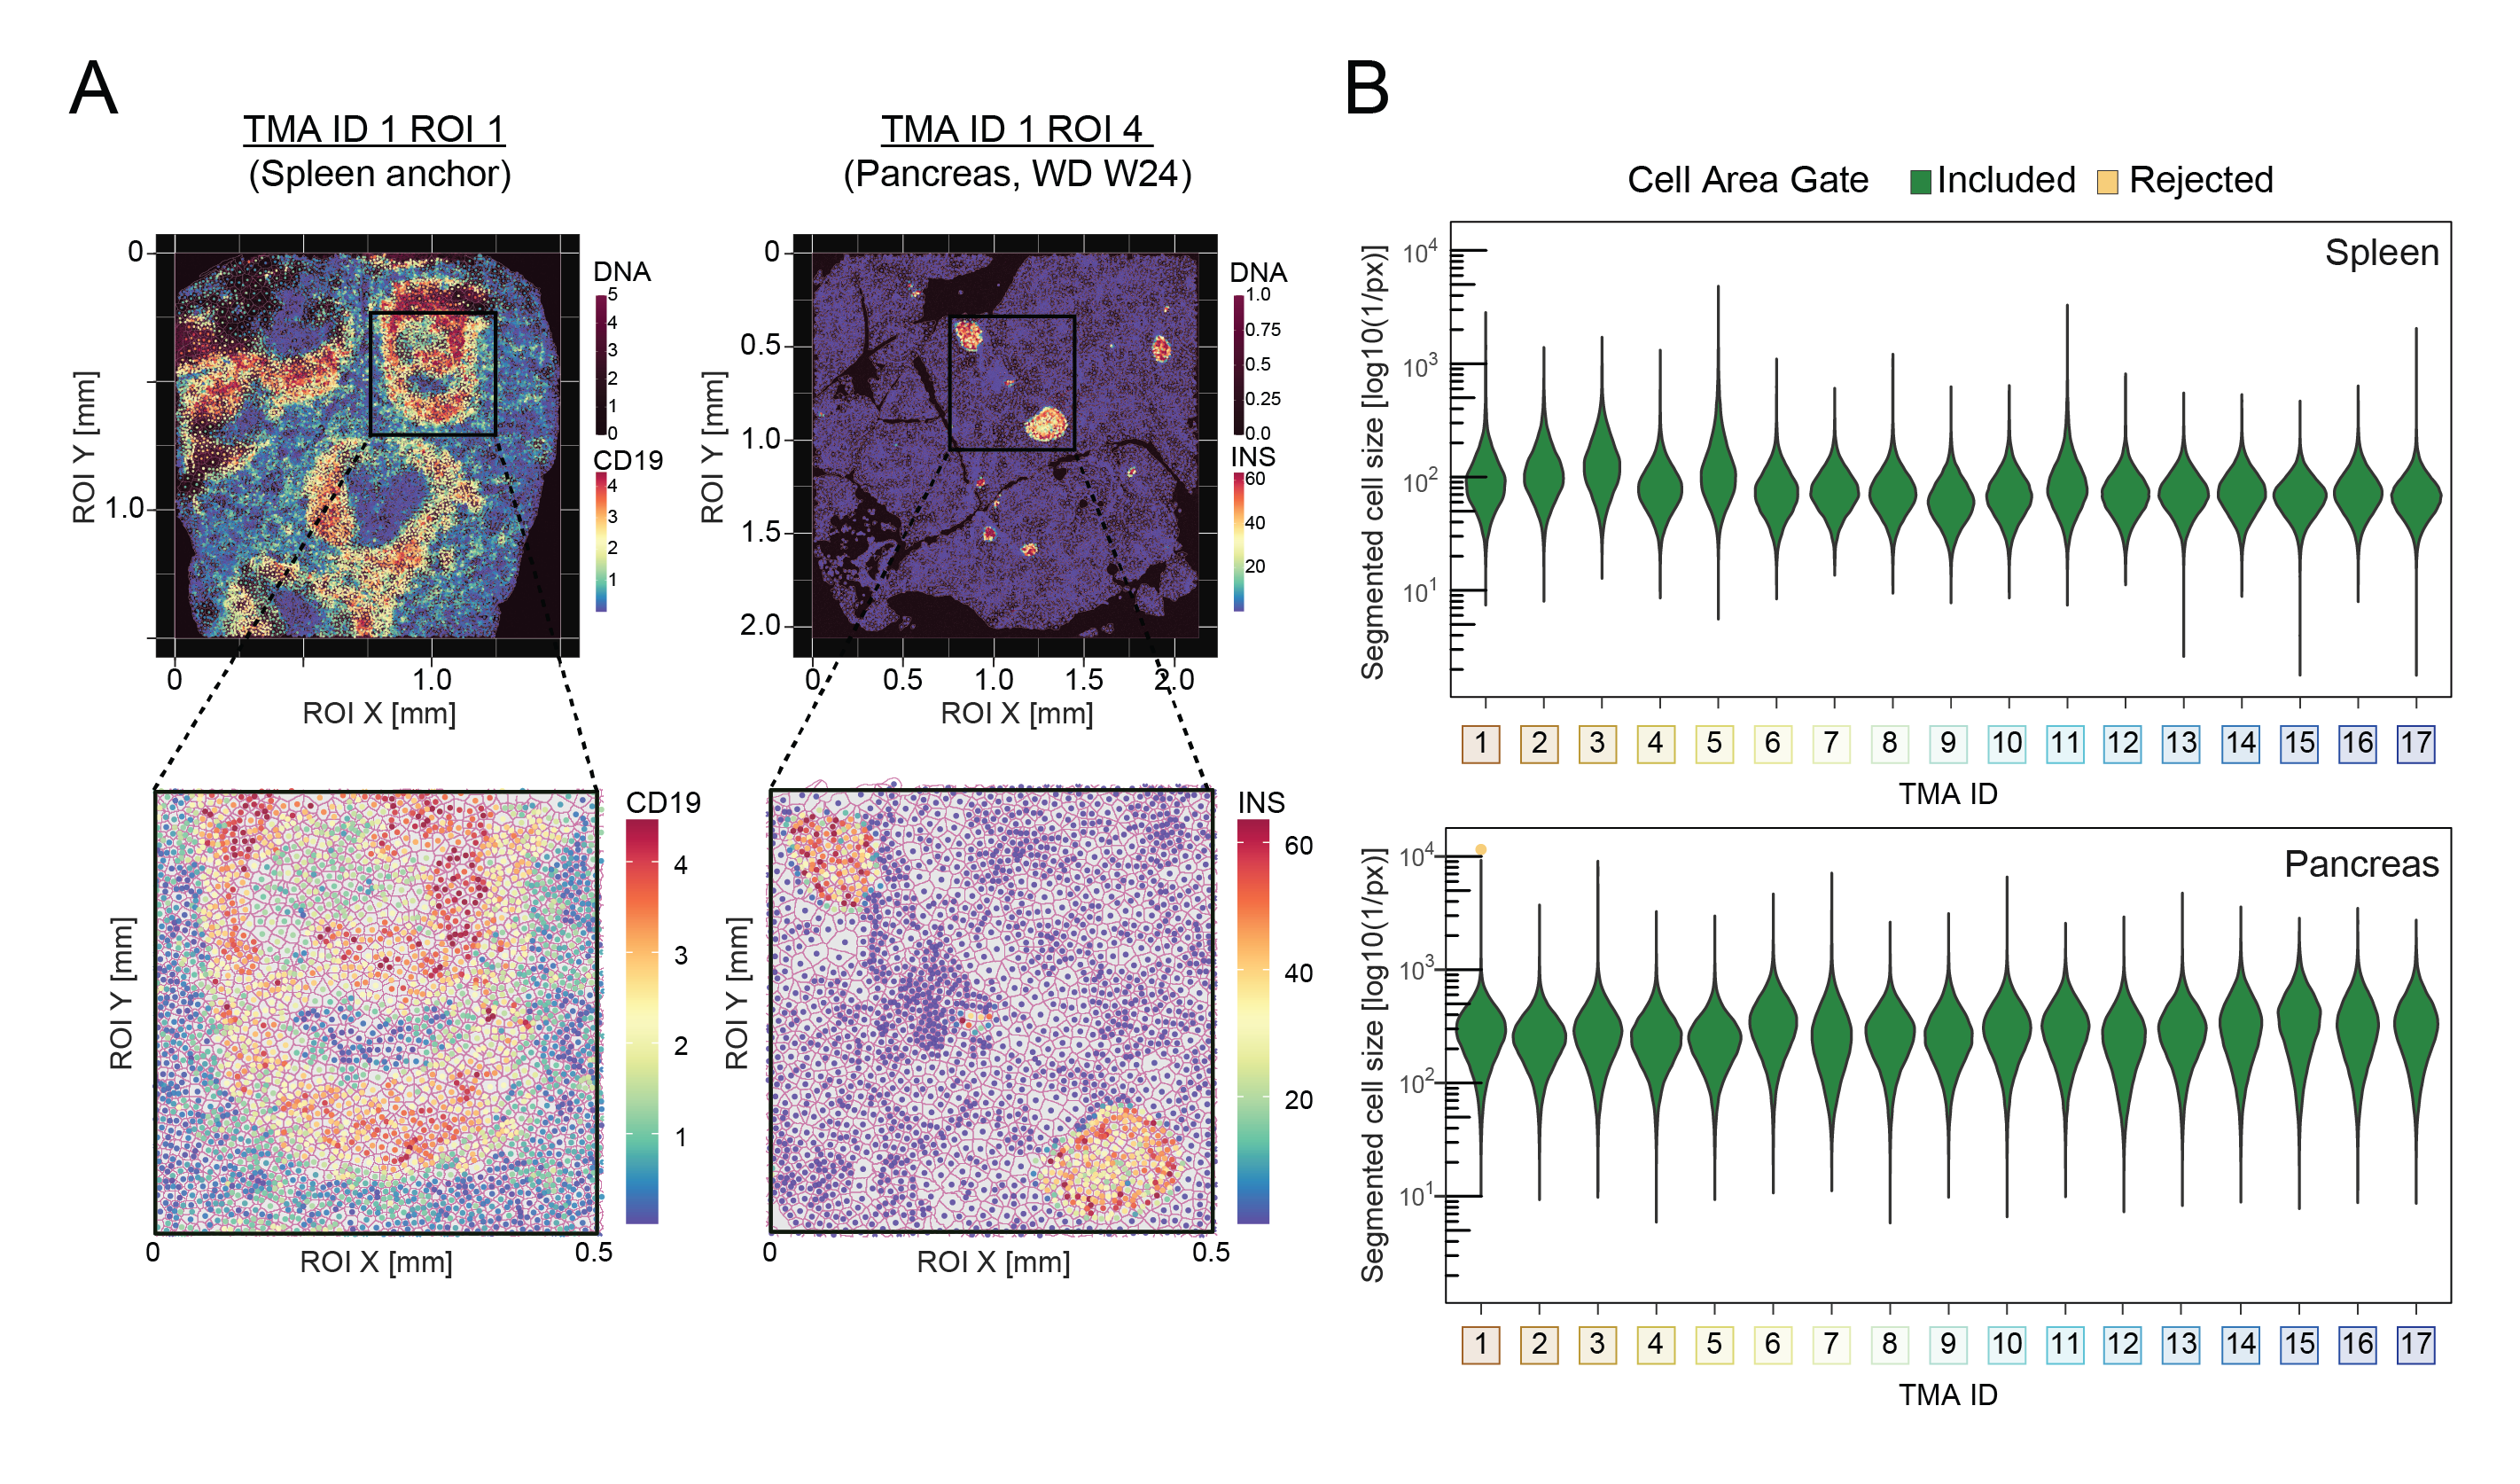
\includegraphics[width=\linewidth]{Appendix2/Fig/F2-A4-01.png}
    \caption[\glsentryshort{imc} Segmentation Workflow]{\textbf{\gls{imc} Segmentation Workflow.} \textbf{(A)} Representative segmentation masks of ablated \glspl{roi} in anchor spleen (left) and pancreas (right) sections, zoomed in to 500 \textmu m on each \gls{roi} for better visibility. For better orientation, average expression of CD19 (left) and INS (right) channles of each segmented cell are additionally drawn as dots. Dimensions of each \gls{roi} are denoted on both axes (1 pixel per \textmu m resolution). \textbf{(B)} Violin plots depicting the $\log\textsubscript{10}$-transformed pixel count (indicating cell size) within each segmented cell across all \glspl{tma} from all analyzed samples. Cells larger than 10000 pixels, potentially representing doublets, are highlighted in yellow and removed from downstream analysis. \textit{This data and figure were originally generated by Dr. Matthias Barone and reused here with permission.}}
    \label{fig:app_imc_segmentation}
\end{figure}

% \begin{figure}[htbp]
%     \centering
%     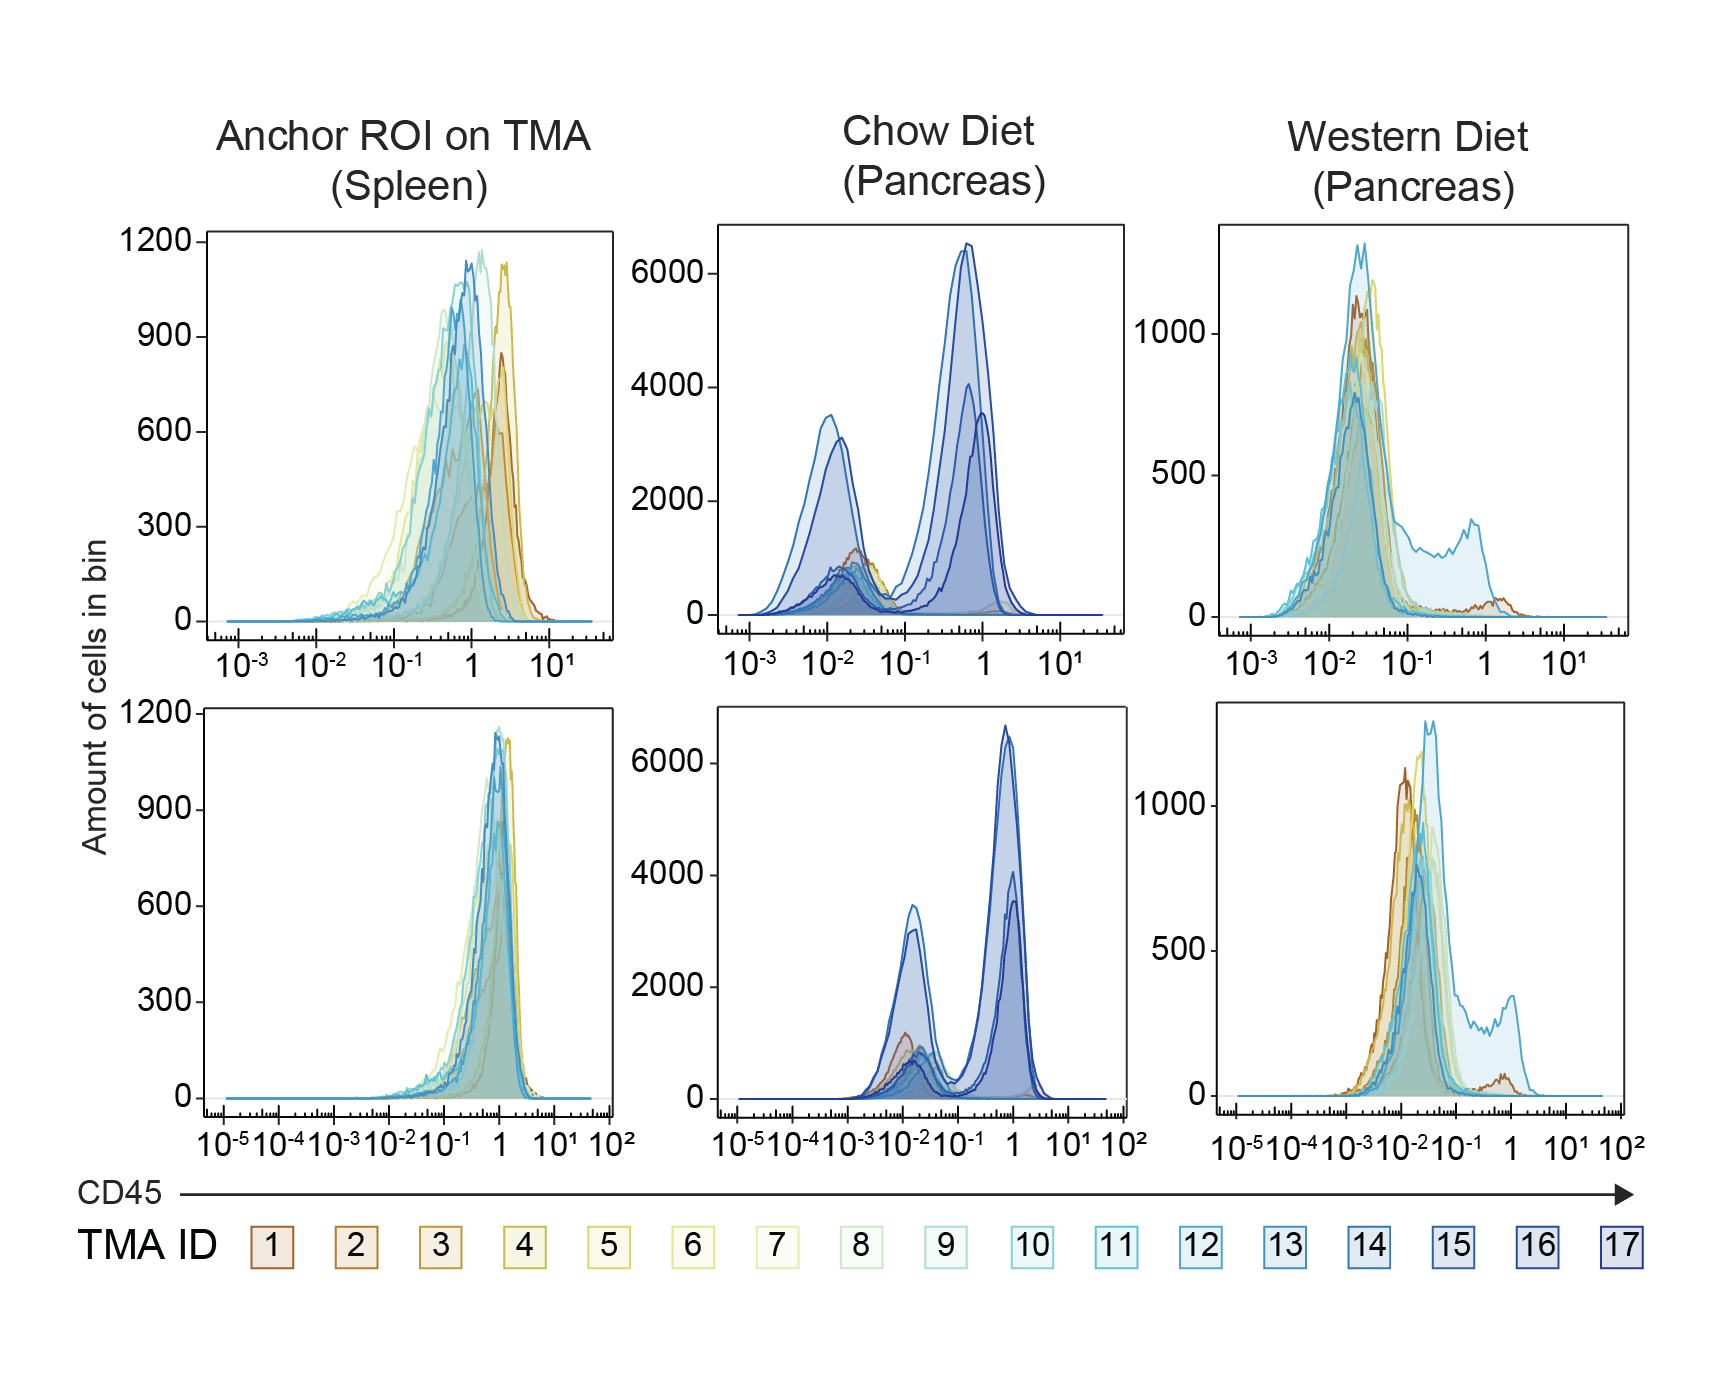
\includegraphics[width=\linewidth]{Appendix2/Fig/F2-A4-02.png}
%     \caption[imc-anchor]{\textbf{Anchor and Batch Correction}}
%     \label{suppl_fig:imc_anchor}
% \end{figure}


\begin{figure}[H]
    \centering
    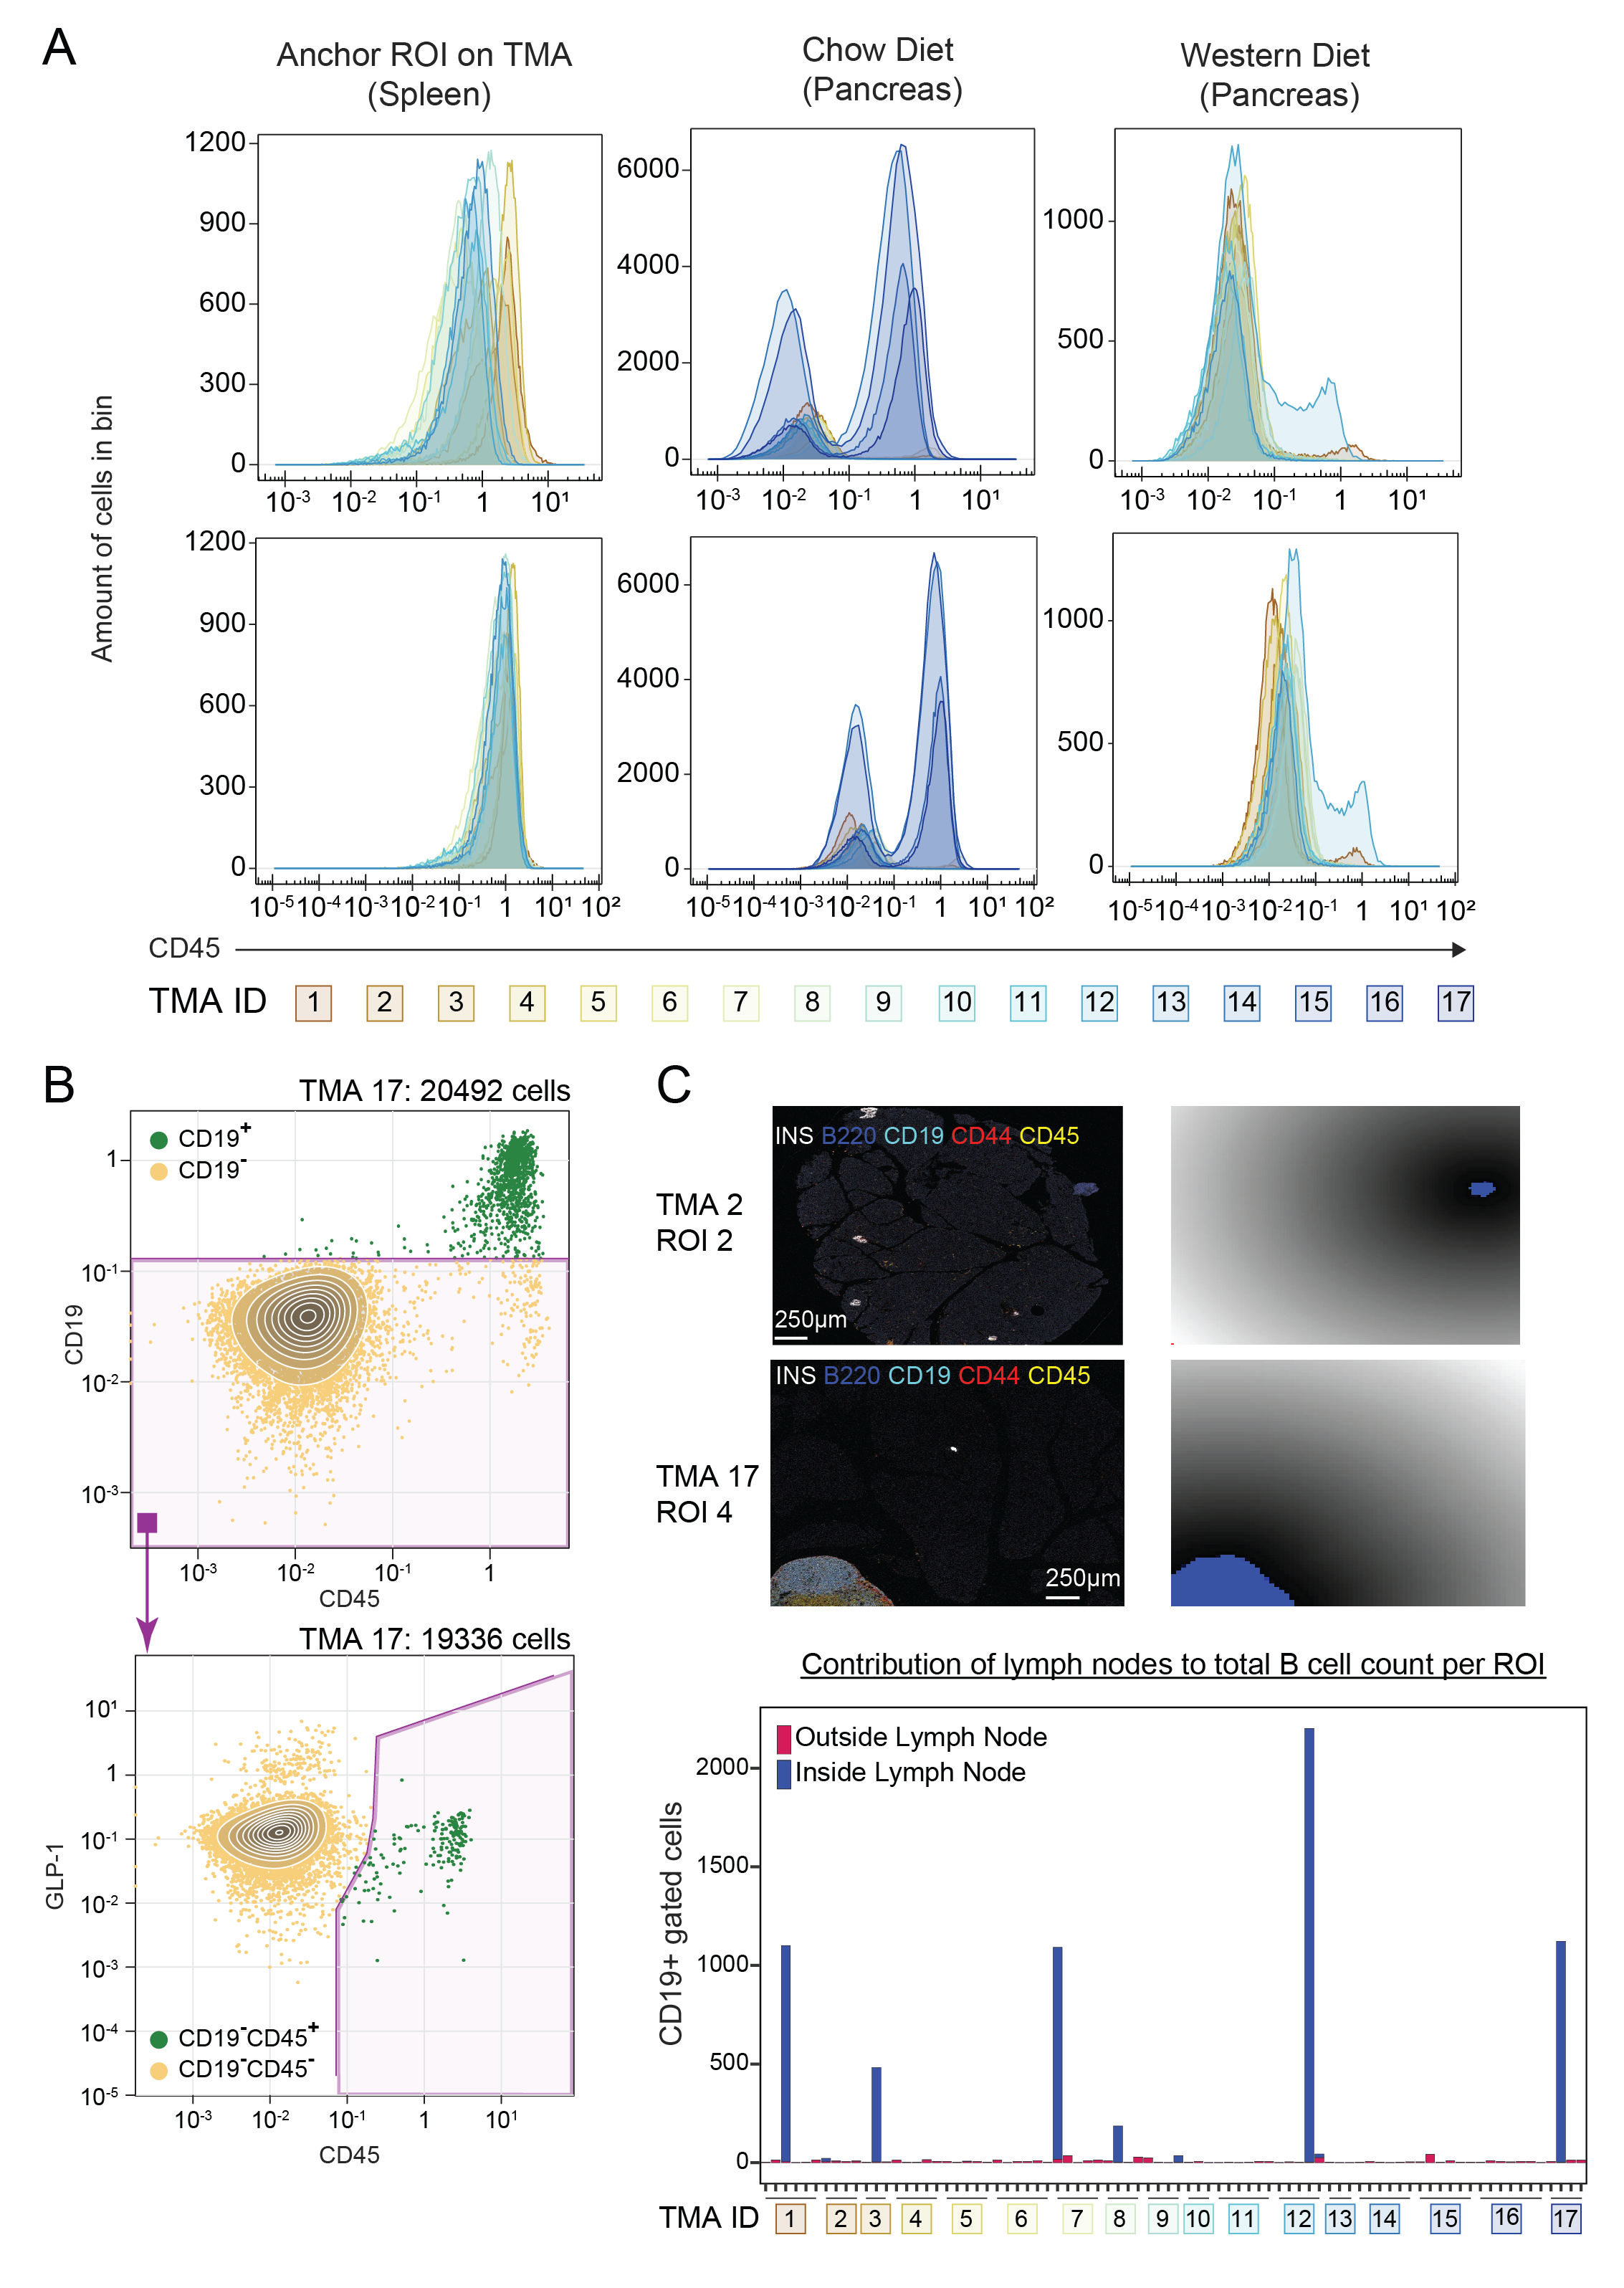
\includegraphics[width=14cm]{Appendix2/Fig/F2-A2-01.png}
    \captionof{figure}[Exclusion of CD19\textsuperscript{+} B-cells]{\textbf{Exclusion of CD19\textsuperscript{+} B-cells}. \textbf{(A)} Histograms showing raw (top) and reference-\gls{roi}-normalized (bottom) \gls{imc} signal intensity from the CD45 channel across all \glspl{tma}. The normalization process involved adjusting every channel across all \glspl{tma} relative to its positive peak intensity on the anchor spleen \gls{roi} of the \gls{tma} (left column). \textbf{(B)} Representative scatter plots depicting the boolean gating strategy employed to identify pancreatic non-B-cell immune cells (CD19\textsuperscript{-}/CD45\textsuperscript{+}/\glslink{glp1}{GLP-1}R\textsuperscript{-}) within each \gls{tma}. \textbf{(C)} Representative \glspl{roi} showing two pancreatic lymph nodes (highlighted in blue, top left). Pancreatic lymph node masks were generated based on a composite overlay of signals from  B220, CD19, CD44, and CD45 (top right), scale bar, 250 \textmu m. Bottom: Bar plot with counts of CD19\textsuperscript{+} B-cells within and outside of the generated lymph node masks. \textit{This data and figure were originally generated by Dr. Matthias Barone and reused here with permission.}}
    %[imc-anchorbcell]{\textbf{Exclusion of CD19+ B-cells}\\
    %\textbf{(A)} Histograms showing raw (top) and normalized (bottom) IMC signal intensity from the CD45 channel across all TMAs. The normalization %process involved adjusting every channel across all TMAs relative to its positive peak intensity on the anchor Spleen ROI of the TMA (left column). \textbf{(B)} Representative scatter plots depicting the boolean gating strategy employed to identify pancreatic non-B-cell immune cells (CD19\textsuperscript{-}/CD45\textsuperscript{+}/GLP-1\textsuperscript{-}) within each TMA. \textbf{(C)} Representative ROIs showing two pancreatic lymph nodes (highlighted in blue, top left). Pancreatic lymph node masks were generated based on a composite overlay of signals from  B220, CD19, CD44, and CD45 (top right, see SI), scale bar, 250 µm. Bottom: Bar plot with counts of CD19\textsuperscript{+} B cells within and outside of tje generated lymph node masks.}
    \label{fig:app_imc_anchorbcell}
\end{figure}


\begin{figure}[H]
    \centering
    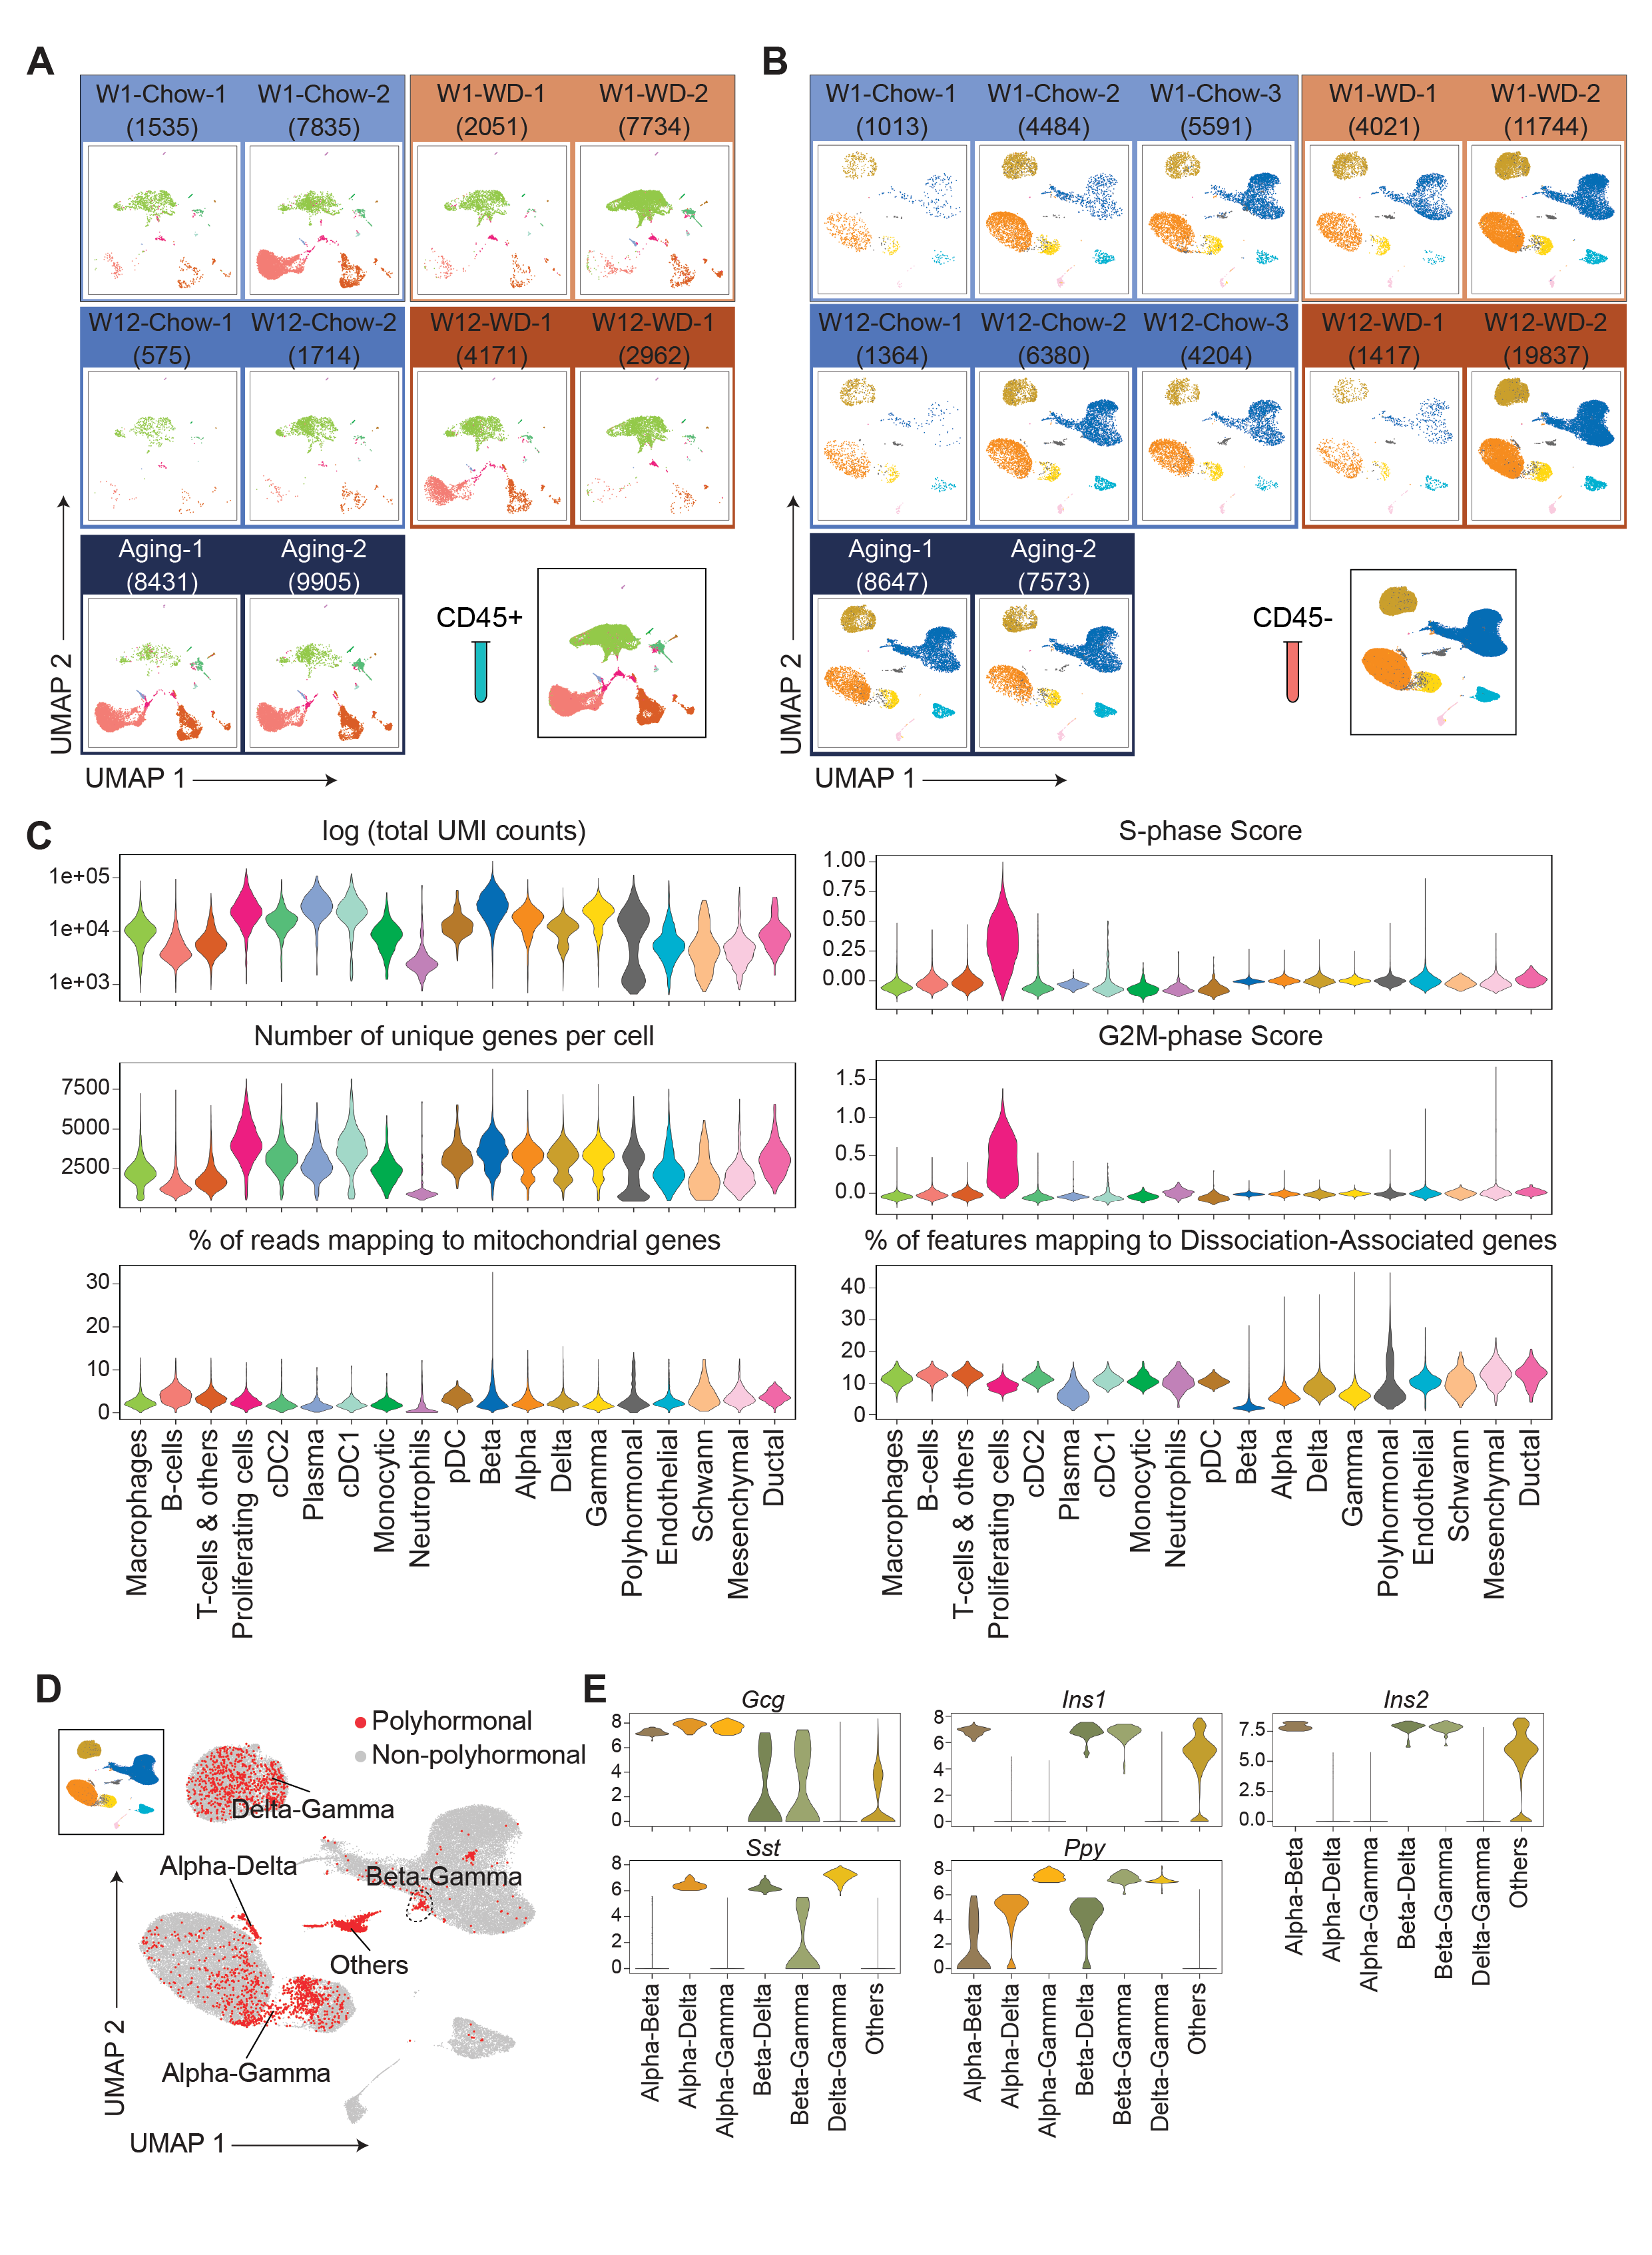
\includegraphics[width=13cm]{Appendix2/Fig/F2-A5-01.png}
    \caption[Quality control of \glsentryshort{scr} data]{\textbf{Quality control of \gls{scr} data}. 
    \textbf{(A,B)} Split view of the CD45\textsuperscript{+} immune cells \textbf{(A)} and CD45\textsuperscript{-} non-immune cells \textbf{(B)} across all cohorts. The number of cells retained in each cohort post quality checks is indicated in parentheses. \textbf{(C)} Violin plots of \gls{qc} metrics for every annotated cell-type after integration –  $\log$ \gls{umi} counts per cell (top left); number of unique features per cell (middle left); percentage of reads mapping to mitochondrial genome (bottom left); cell-cycle phase scores (top and middle right) and dissociation-associated genes (bottom-right) \textbf{(D)} \gls{umap} embedding of `Endocrine \& Others' cells depicting the identified polyhormonal populations (in red). The non-polyhormonal cells are depicted in grey. \textbf{(E)} Violin plots of the five primary islet hormone markers across the identified polyhormonal cells in \textbf{(D)}. The number of cells pre-\gls{qc} in each cohort can be found in \textbf{\autoref{tab:app_scrna_meta}}}.
    \label{fig:app_scrna_qc}
\end{figure}

\begin{figure}[H]
    \centering
    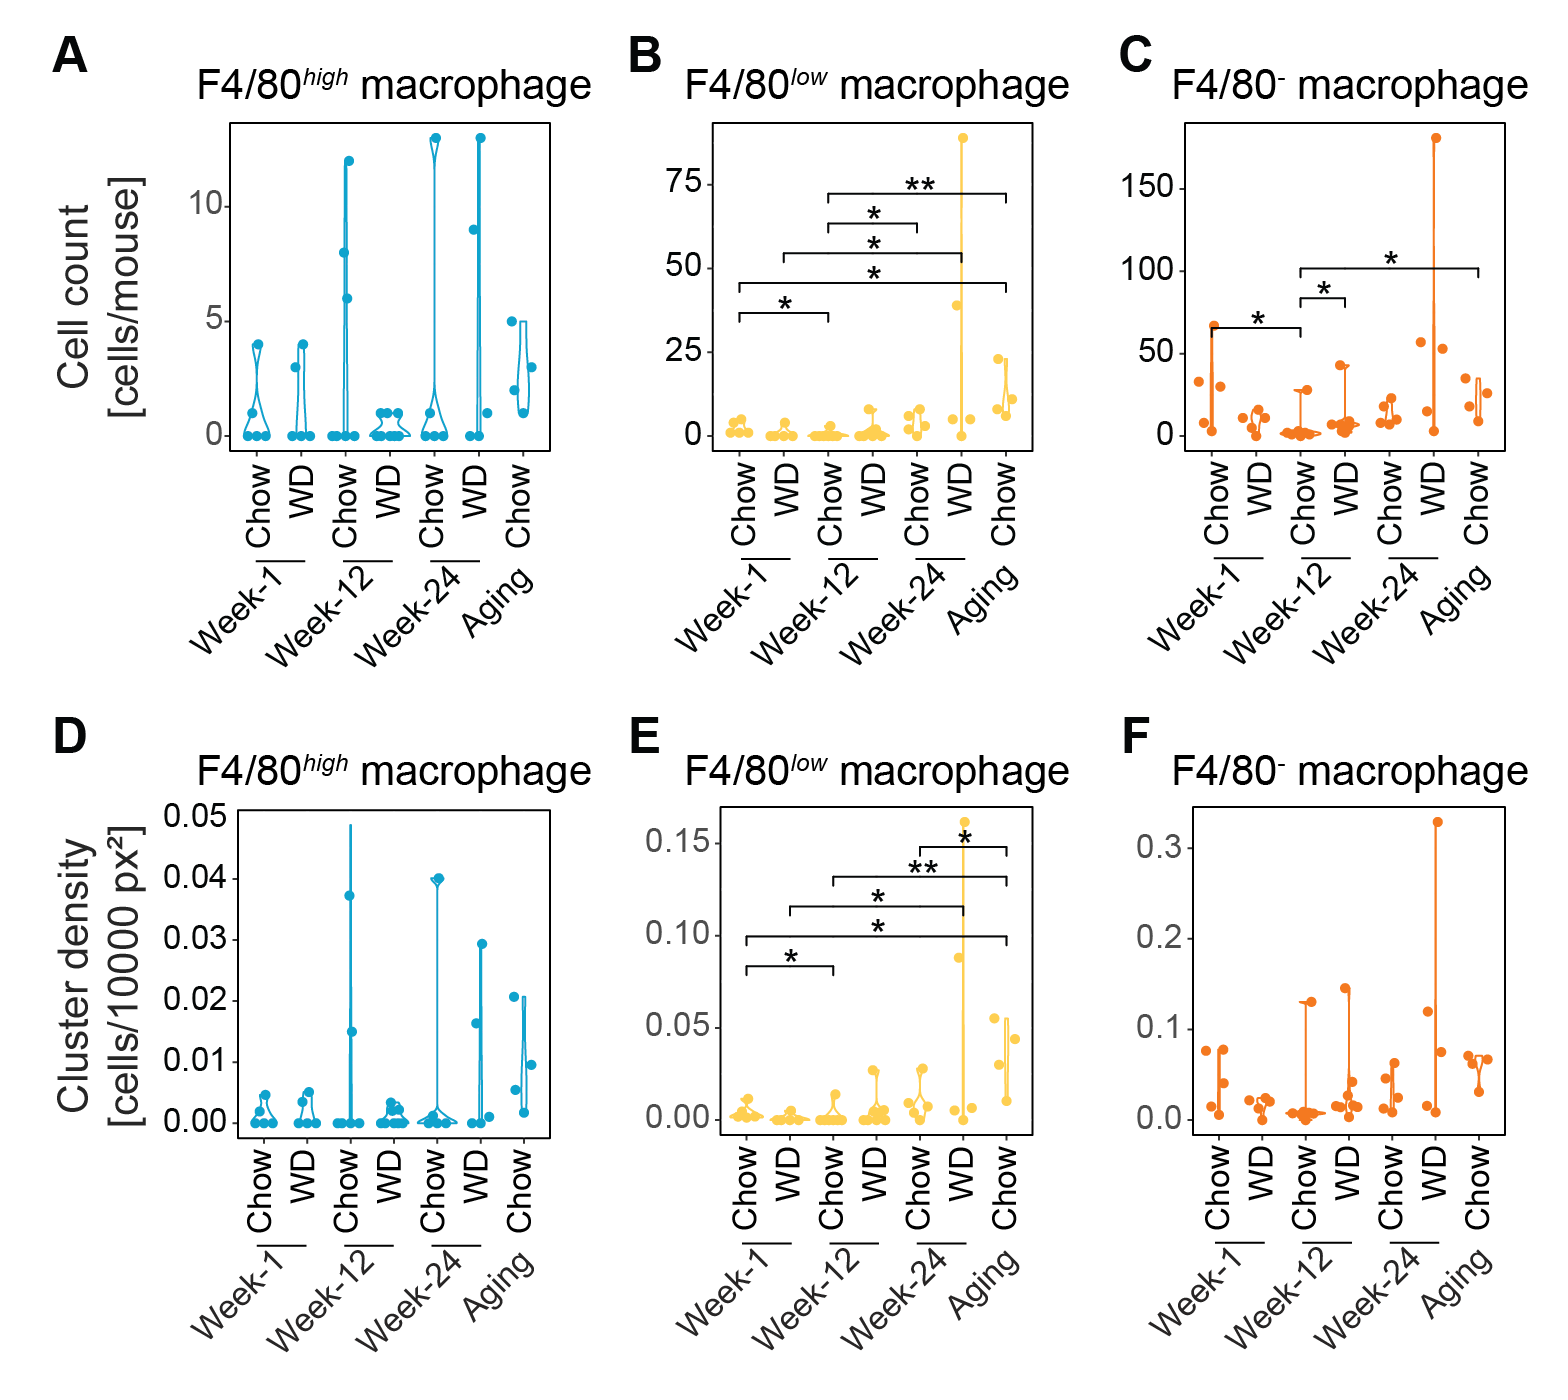
\includegraphics[width=\linewidth]{Appendix2/Fig/F2-A3-01.png}
    \caption[Cell count and density of F4/80 macrophages from \glsentryshort{imc} analysis]{\textbf{Cell count and density of F4/80\textsuperscript{\textit{high}}, F4/80\textsuperscript{\textit{low}} and F4/80\textsuperscript{-} macrophage sub-populations.} \textbf{(A-C)} Violin plots displaying the total counts of F4/80\textsuperscript{\textit{high}} \textbf{(A)}, F4/80\textsuperscript{\textit{low}} \textbf{(B)} and F4/80\textsuperscript{\textit{-}} \textbf{(C)} macrophages in non-lymph node pancreatic regions in each mouse across various experimental conditions. \textbf{(D-F)} Violin plots displaying the section-size normalized counts of F4/80\textsuperscript{\textit{high}} \textbf{(D)}, F4/80\textsuperscript{\textit{low}} \textbf{(E)} and F4/80\textsuperscript{\textit{-}} \textbf{(F)} macrophages in non-lymph node pancreatic regions in each mouse across various experimental conditions. $\textsuperscript{*} p < 0.05, \textsuperscript{**} p < 0.01$. p-values were calculated using the Wilcoxon rank-sum test. \textit{This data and figure were originally generated by Dr. Matthias Barone and reused here with permission.}}
    \label{fig:app_imc_macrophages}
\end{figure}

% \begin{figure}[H]
%     \centering
%     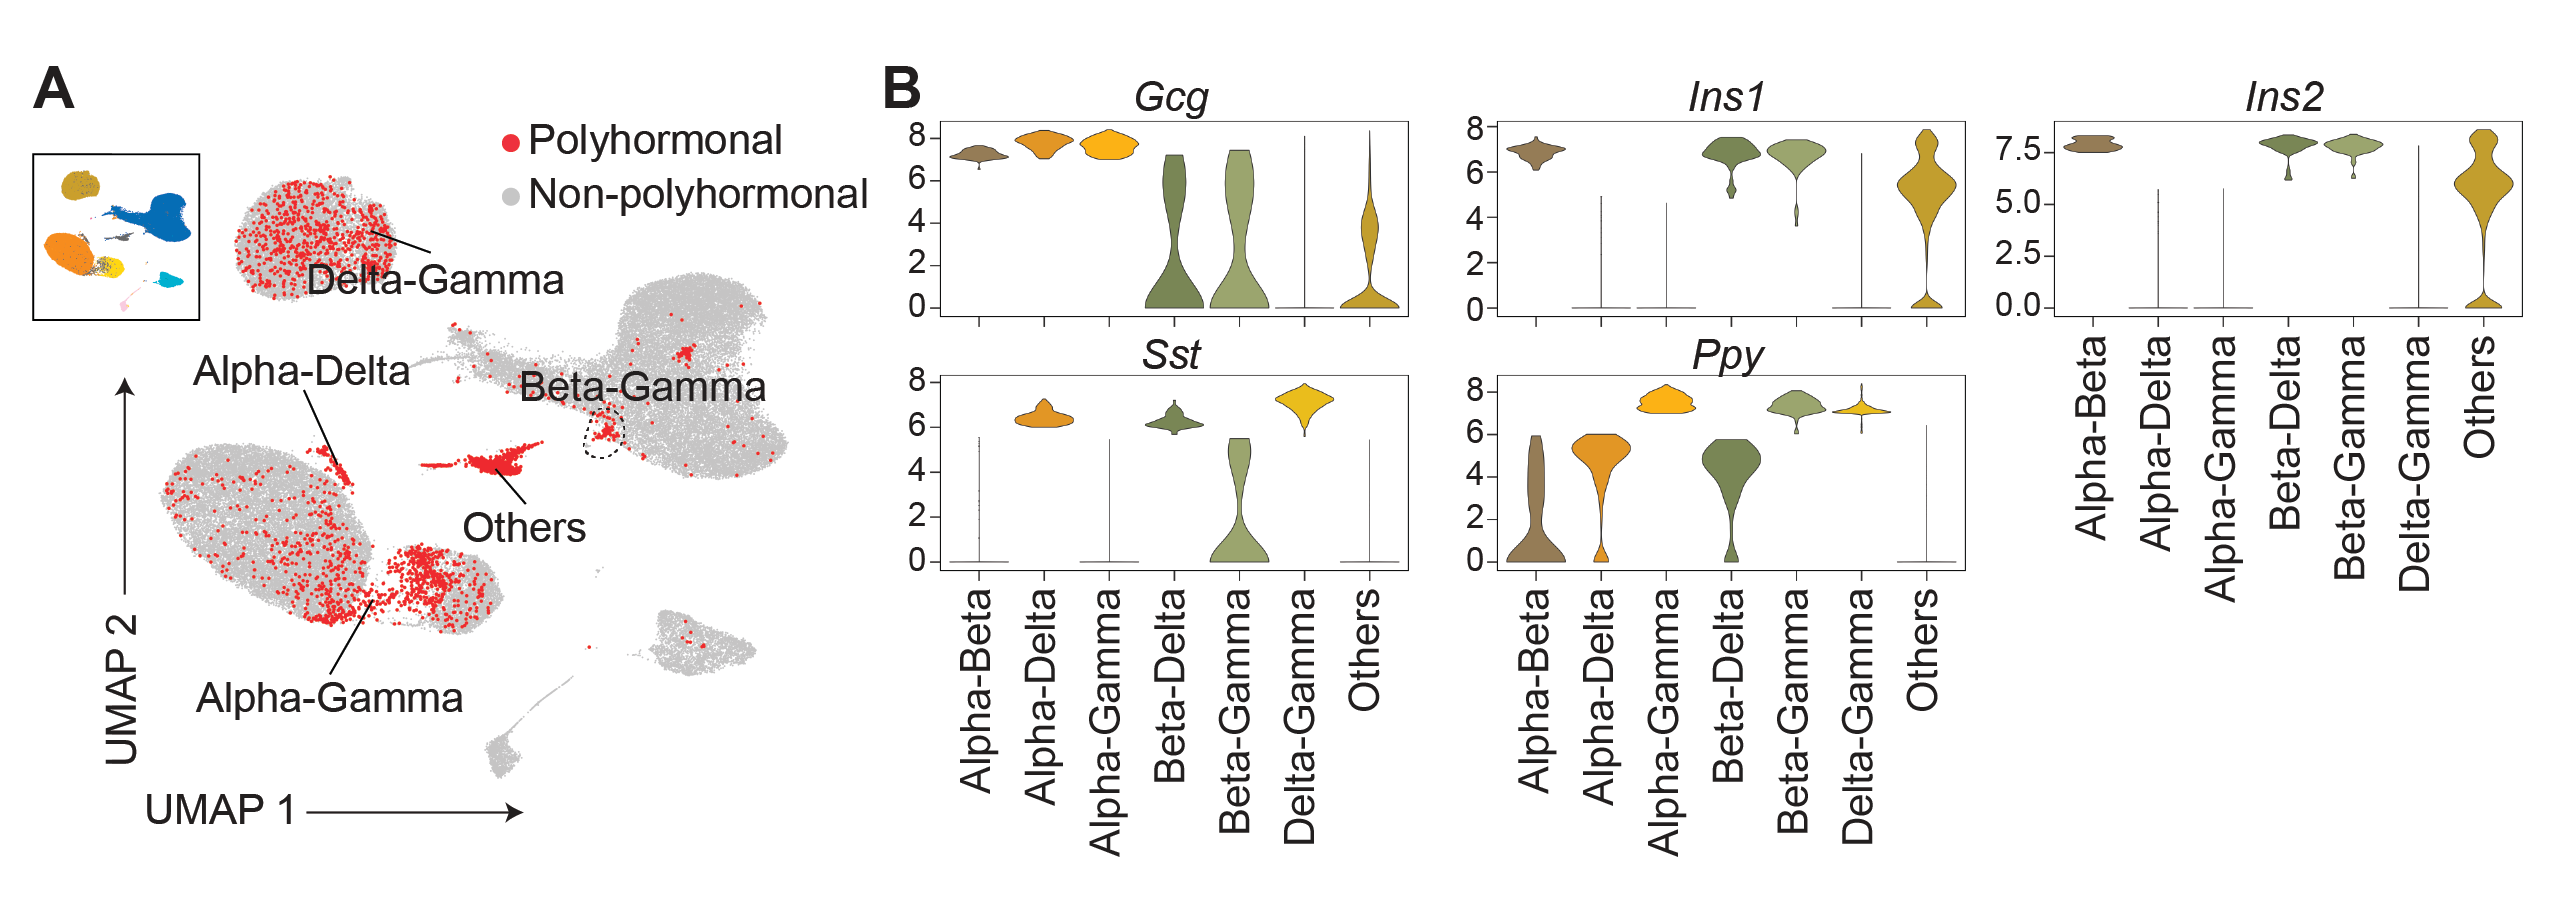
\includegraphics[width=\linewidth]{Appendix2/Fig/F2-A6-01.png}
%     \caption[suppl-fig:sc-endo]{\textbf{Annotating Polyhormonal cells}\\
%     \textbf{(A)} UMAP embedding of Endocrine \& Others' from \textbf{Fig.\ref{fig2-3} C} depicting the identified polyhormonal populations (in red). The non-polyhormonal cells are depicted in grey. The \textbf{(B)} Violin plots of the five primary islet hormone markers across the identified polyhormonal populations in \textbf{(A)}}
%     \label{suppl_fig:sc_endo}
% \end{figure}


\begin{figure}[H]
    \centering
    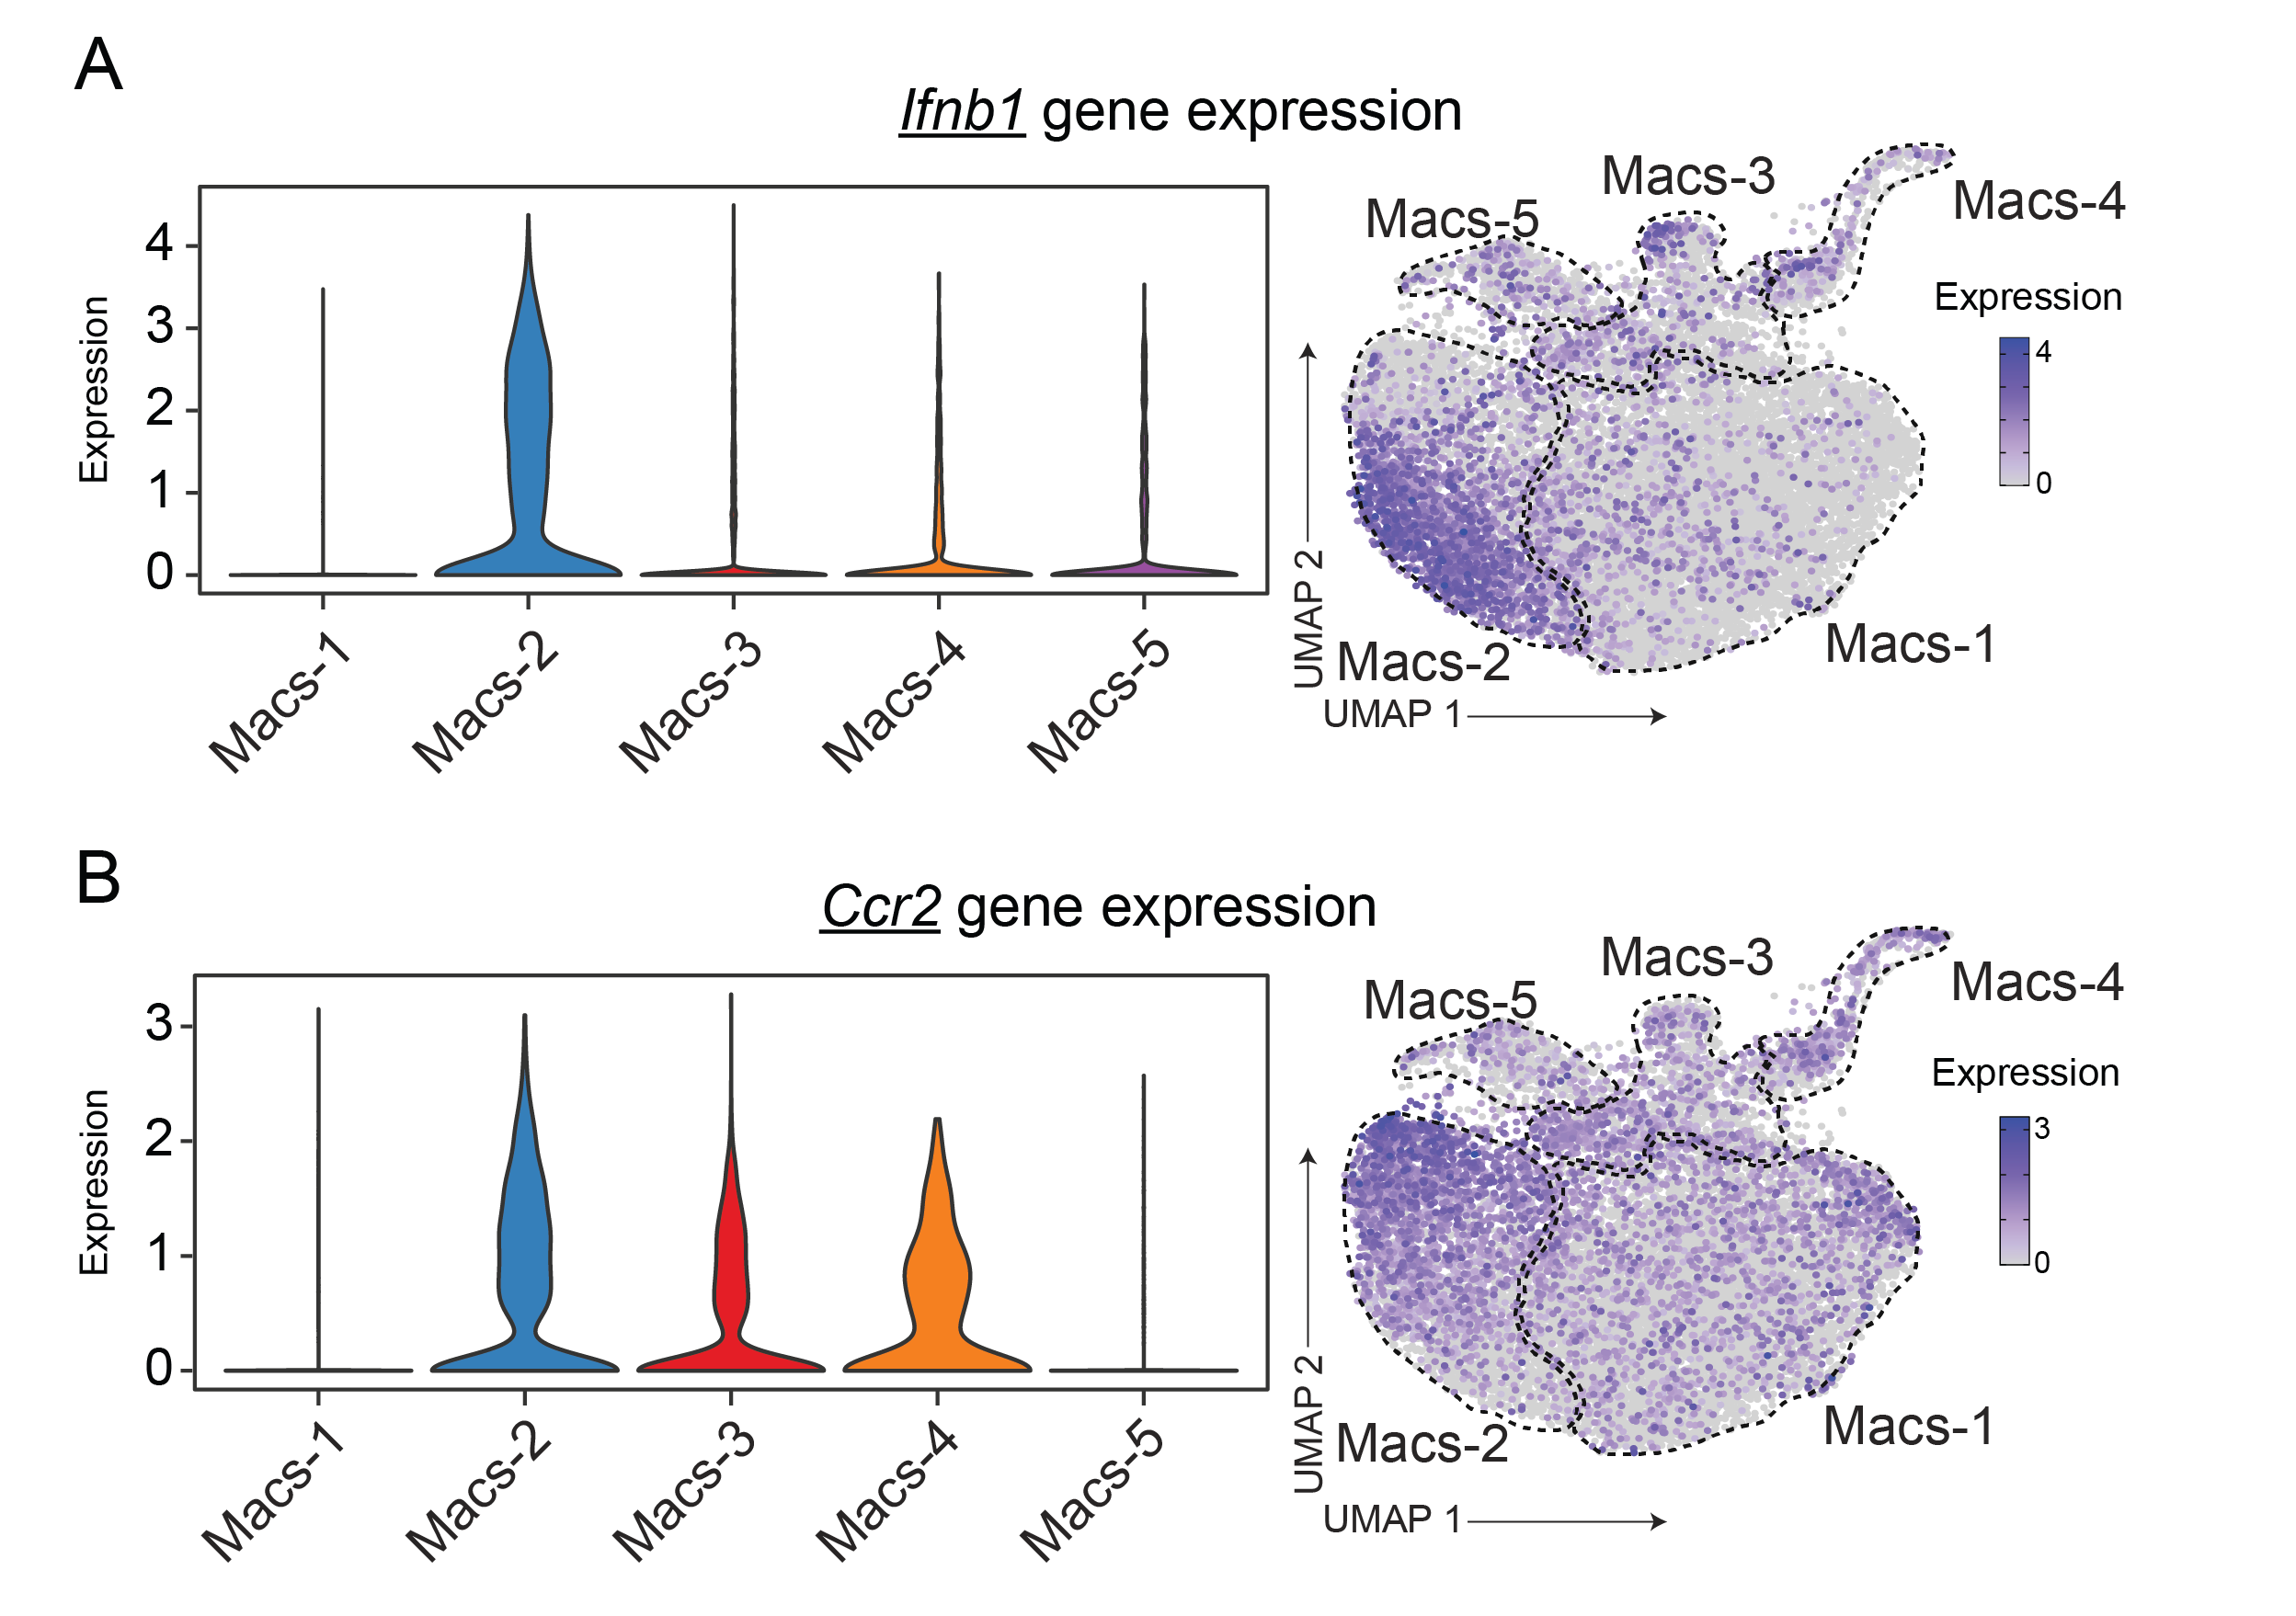
\includegraphics[width=12cm]{Appendix2/Fig/F2-A7-01.png}
    \caption[Gene expression across macrophages sub-populations]{\textbf{Gene expression across macrophages sub-populations.} \textbf{(A) - (B)} Violin plot (left) and feature plot (right) depicting the expression of \textit{Ifnb1} \textbf{(A)} and \textit{Ccr2} \textbf{(B)} genes in the five macrophage sub-populations in the \gls{scr} data.}
    \label{fig:app_scrna_macrophages_macs2_genes}
\end{figure}


\vspace{-22pt}


\begin{figure}[H]
    \centering
    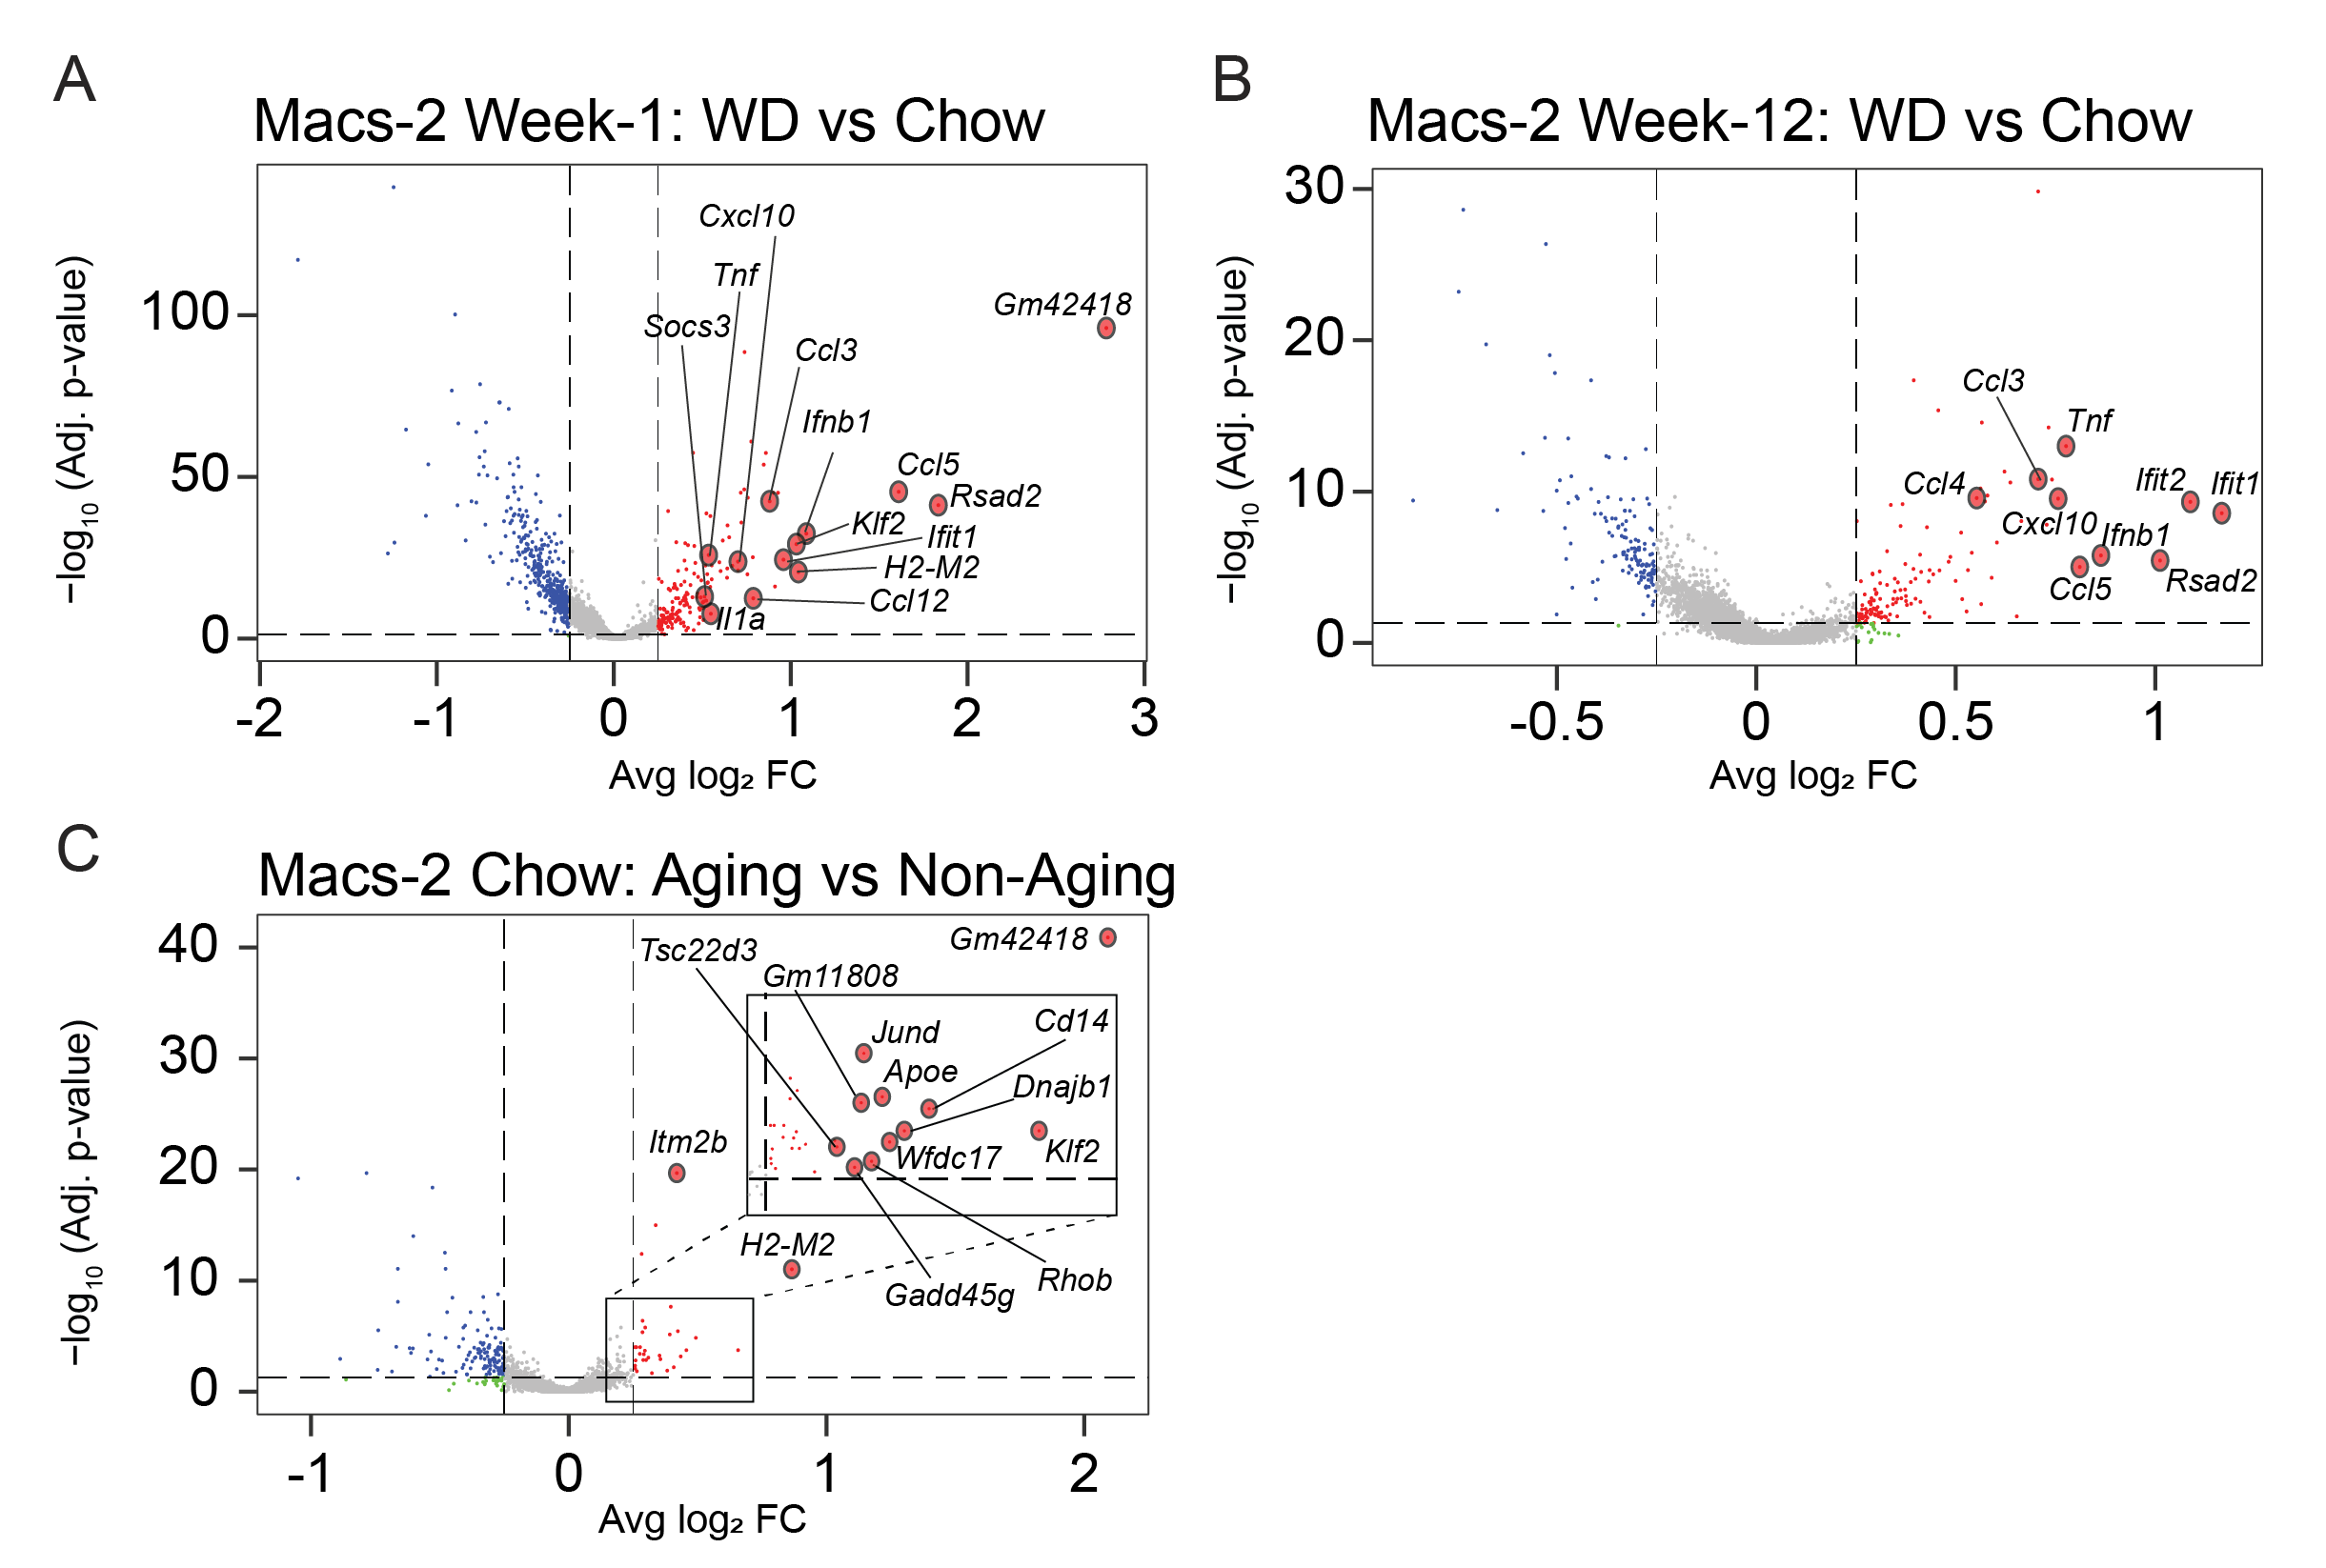
\includegraphics[width=13cm]{Appendix2/Fig/F2-A7-02.png}
    \caption[\glsentryshort{dge} analysis in Macs-2 macrophages]{\textbf{\gls{dge} analysis in Macs-2 macrophages.} \textbf{(A) - (C)} Volcano plots showing \gls{de} genes in Macs-2 macrophage sub-population comparing \gls{wd} versus chow diet at Week-1 \textbf{(A)}, \gls{wd} versus chow diet at Week-12 \textbf{(B)} time-points and chow diet-fed aging cohort versus chow diet-fed non-aging (W1 + W12) cohorts \textbf{(C)}. The dashed vertical lines represent $  \left|Avg. \log FC \right| $ = 0.25 and the dashed horizontal line represent $-\log_{10}(\num{0.05}) = 1.3$. Differentially up-regulated and down-regulated genes are depicted by red and blue dots respectively. Abbreviations: \gls{wd}, western diet; $Avg. \log\textsubscript{2} \gls{fc}$, $\log\textsubscript{2}$ \glsentrylong{fc} of the average expression of the gene between the two groups; Adj. p-value, adjusted p-value based on Bonferroni correction using all genes in the dataset.}
    \label{fig:app_scrna_macrophages_macs2_dge}
\end{figure}

\begin{comment}
\begin{figure}[H]
    \centering
    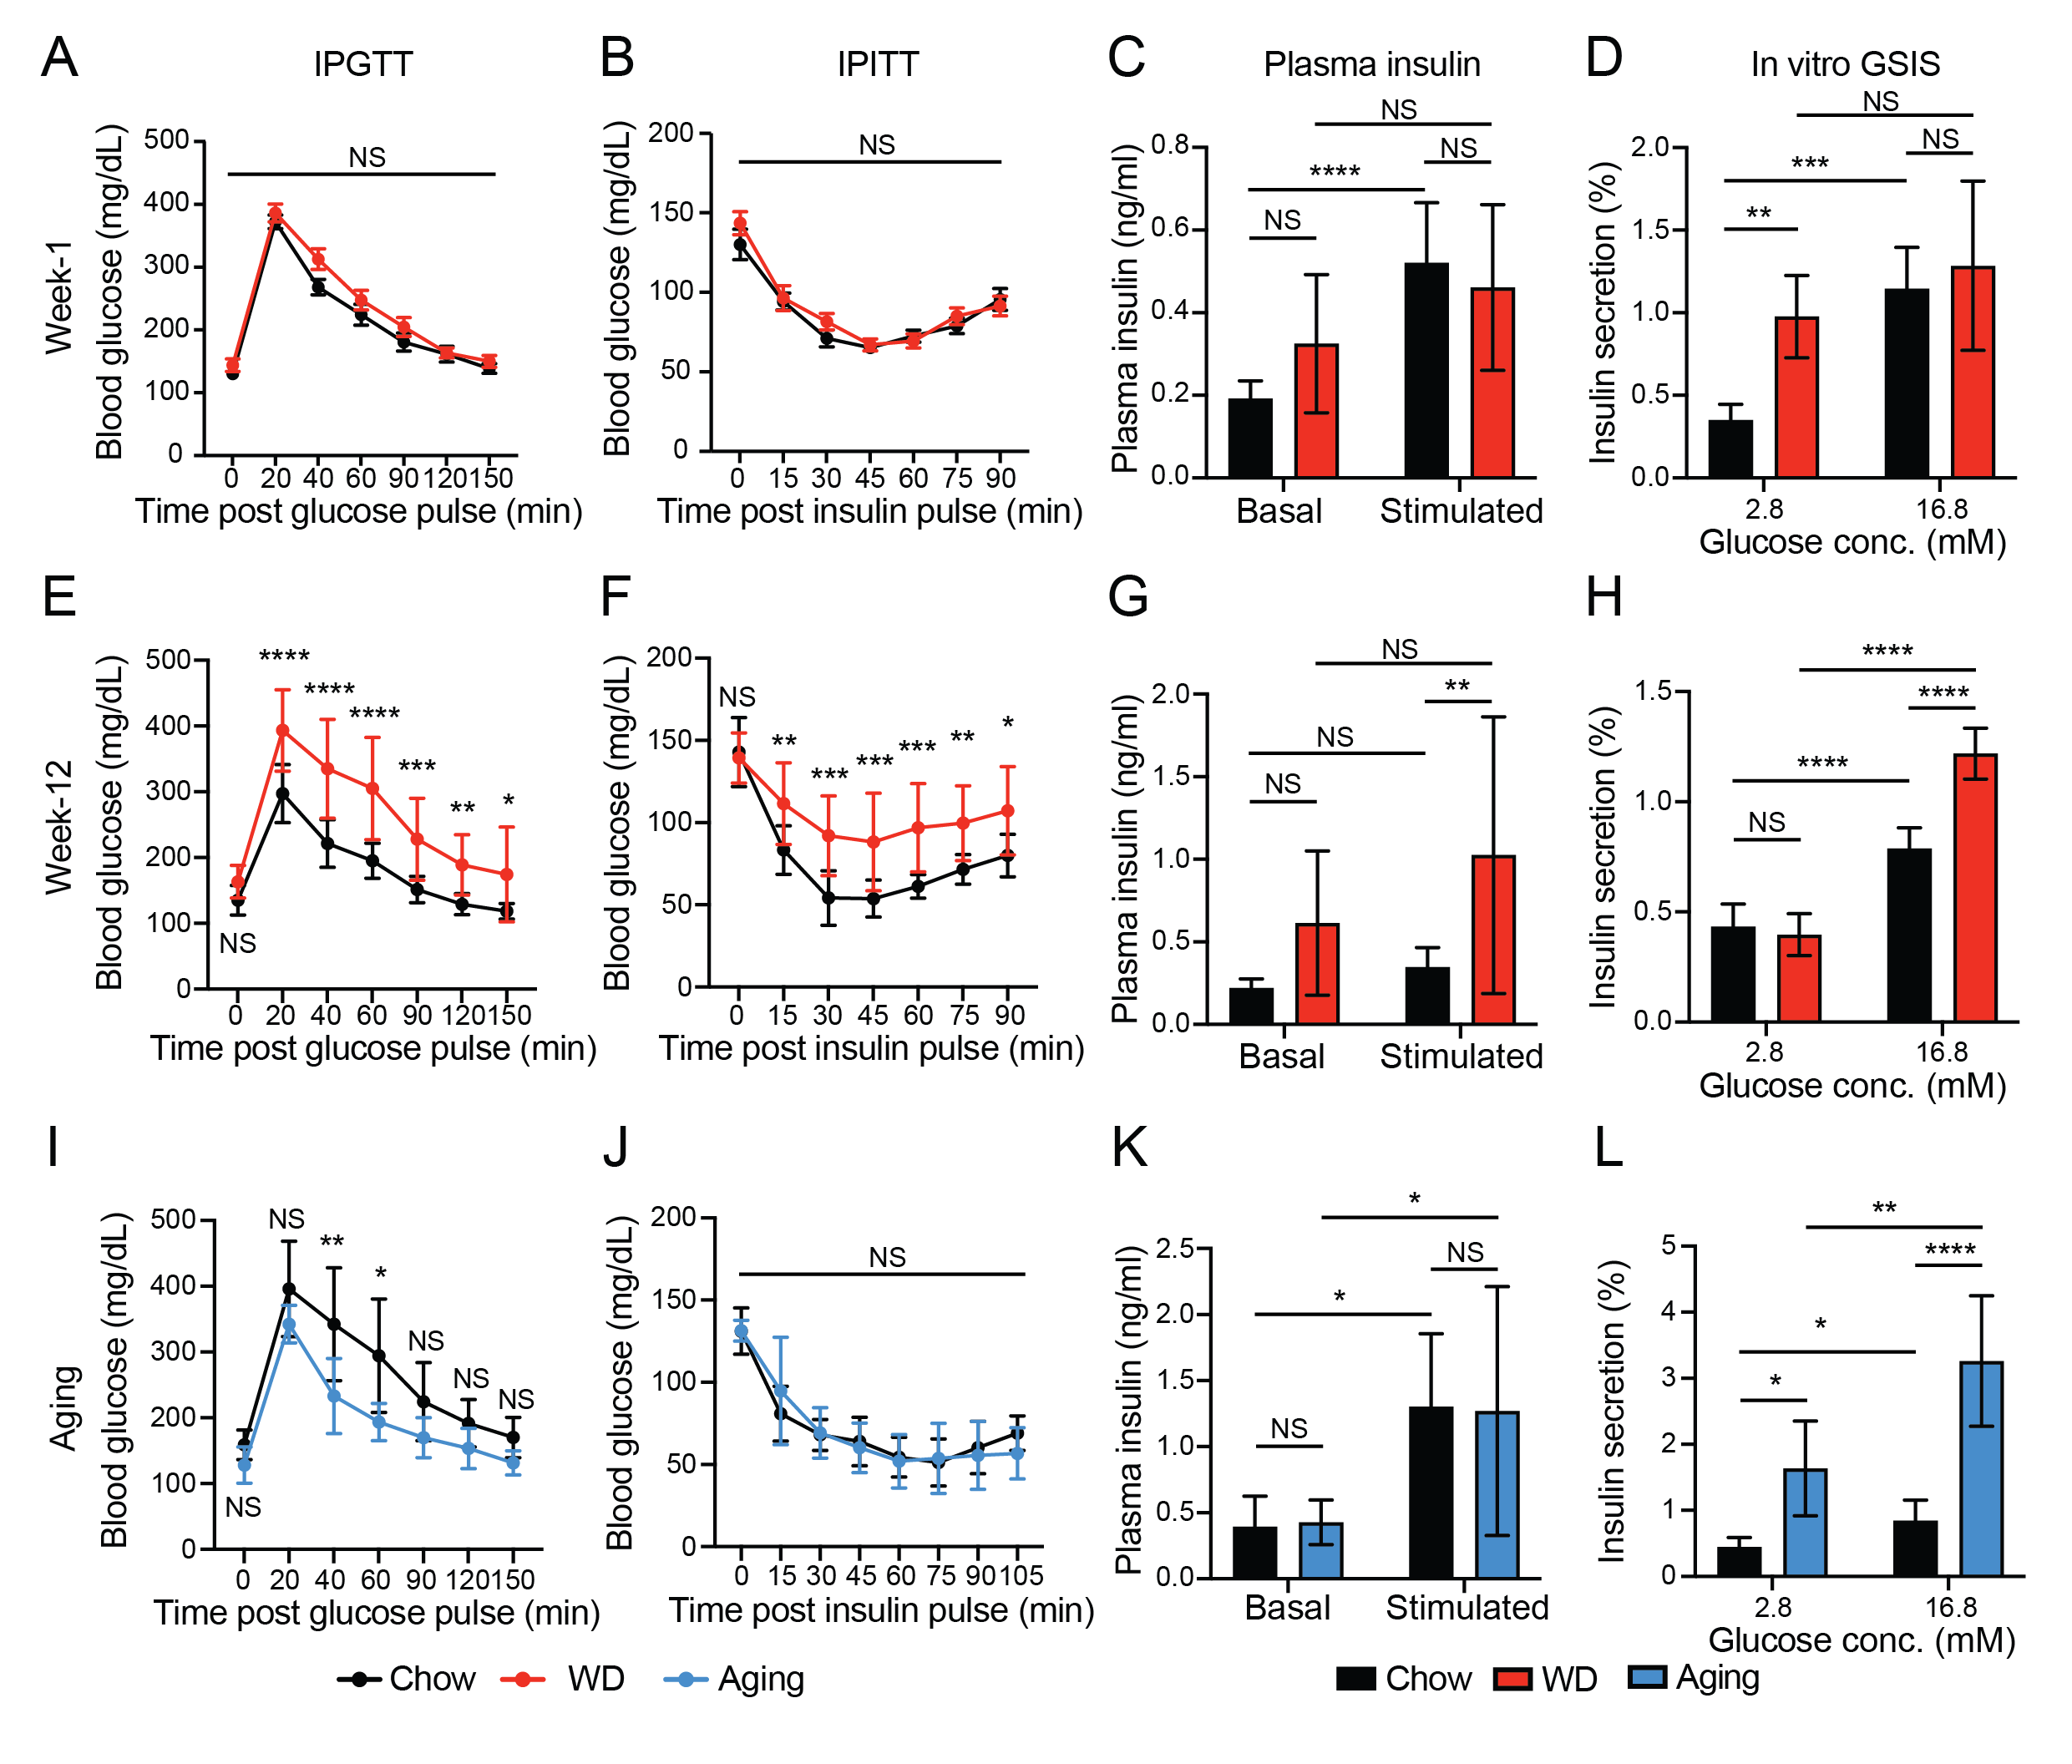
\includegraphics[width=\linewidth]{Appendix2/Fig/F2-A9-01.png}
    \caption[Functional characterization of $\beta$-cells across \glslink{wd}{WD} feeding and aging]{\textbf{Functional characterizations of pancreatic $\beta$-cells across \glslink{wd}{WD} feeding and aging.} \textbf{(A)} Glucose tolerance tests in mice fed with chow diet (n=10) and \gls{wd} (n=10) for one week. \textbf{(B)} Insulin tolerance tests in mice fed with chow diet (n=10) and \gls{wd} (n=10) for one week. \textbf{(C)} Insulin secretion assay in mouse islets post one-week chow diet or \gls{wd}, stimulated at varying glucose concentrations. n=6 (10 islets/pool). \textbf{(D)} Serum insulin levels in mice pre- and post-glucose injection, compared between chow diet fed (n=10) and \gls{wd} fed (n=10) groups over one week. \textbf{(E)} Glucose tolerance tests in mice fed with chow diet (n=10) and \gls{wd} (n=10) for twelve weeks. \textbf{(F)} Insulin tolerance tests in mice fed with chow diet (n=10) and \gls{wd} (n=10) for twelve weeks. \textbf{(G)} Insulin secretion assay in mouse islets post twelve-week chow diet or \gls{wd}, stimulated at varying glucose concentrations. n=6 (10 islets/pool). \textbf{(H)} Serum insulin levels in mice pre- and post-glucose injection, compared between chow diet fed (n=10) and \gls{wd} fed (n=10) groups over twelve weeks. \textbf{(I)} Glucose tolerance tests in adult (n=10, <3-month-old) and aging (n=10, 2-year-old) mice. \textbf{(J)} Insulin tolerance tests in adult (n=10, <3-month-old) and aging (n=10, 2-year-old) mice. \textbf{(K)} Insulin secretion assay in islets from adult (n=10, <3-month-old) and aging (n=10, 2-year-old) mice, stimulated at varying glucose concentrations. n=6 (10 islets/pool). \textbf{(L)} Serum insulin levels in mice pre- and post-glucose injection, compared between adult (n=10, <3-month-old) and aging (n=10, 2-year-old) mice.  $\textsuperscript{*} p < 0.05, \textsuperscript{**} p < 0.01, \textsuperscript{***} p < 0.001, \textsuperscript{****} p < 0.0001, $ NS, not significant, based on multiple comparisons following two-way \glslink{anova}{ANOVA}. \textit{This data and figure were originally generated by Dr. Han Zhu and reused here with permission.}}
    \label{fig:app_metab_betacells}
\end{figure}
\clearpage
\begin{figure}[H]
    \centering
    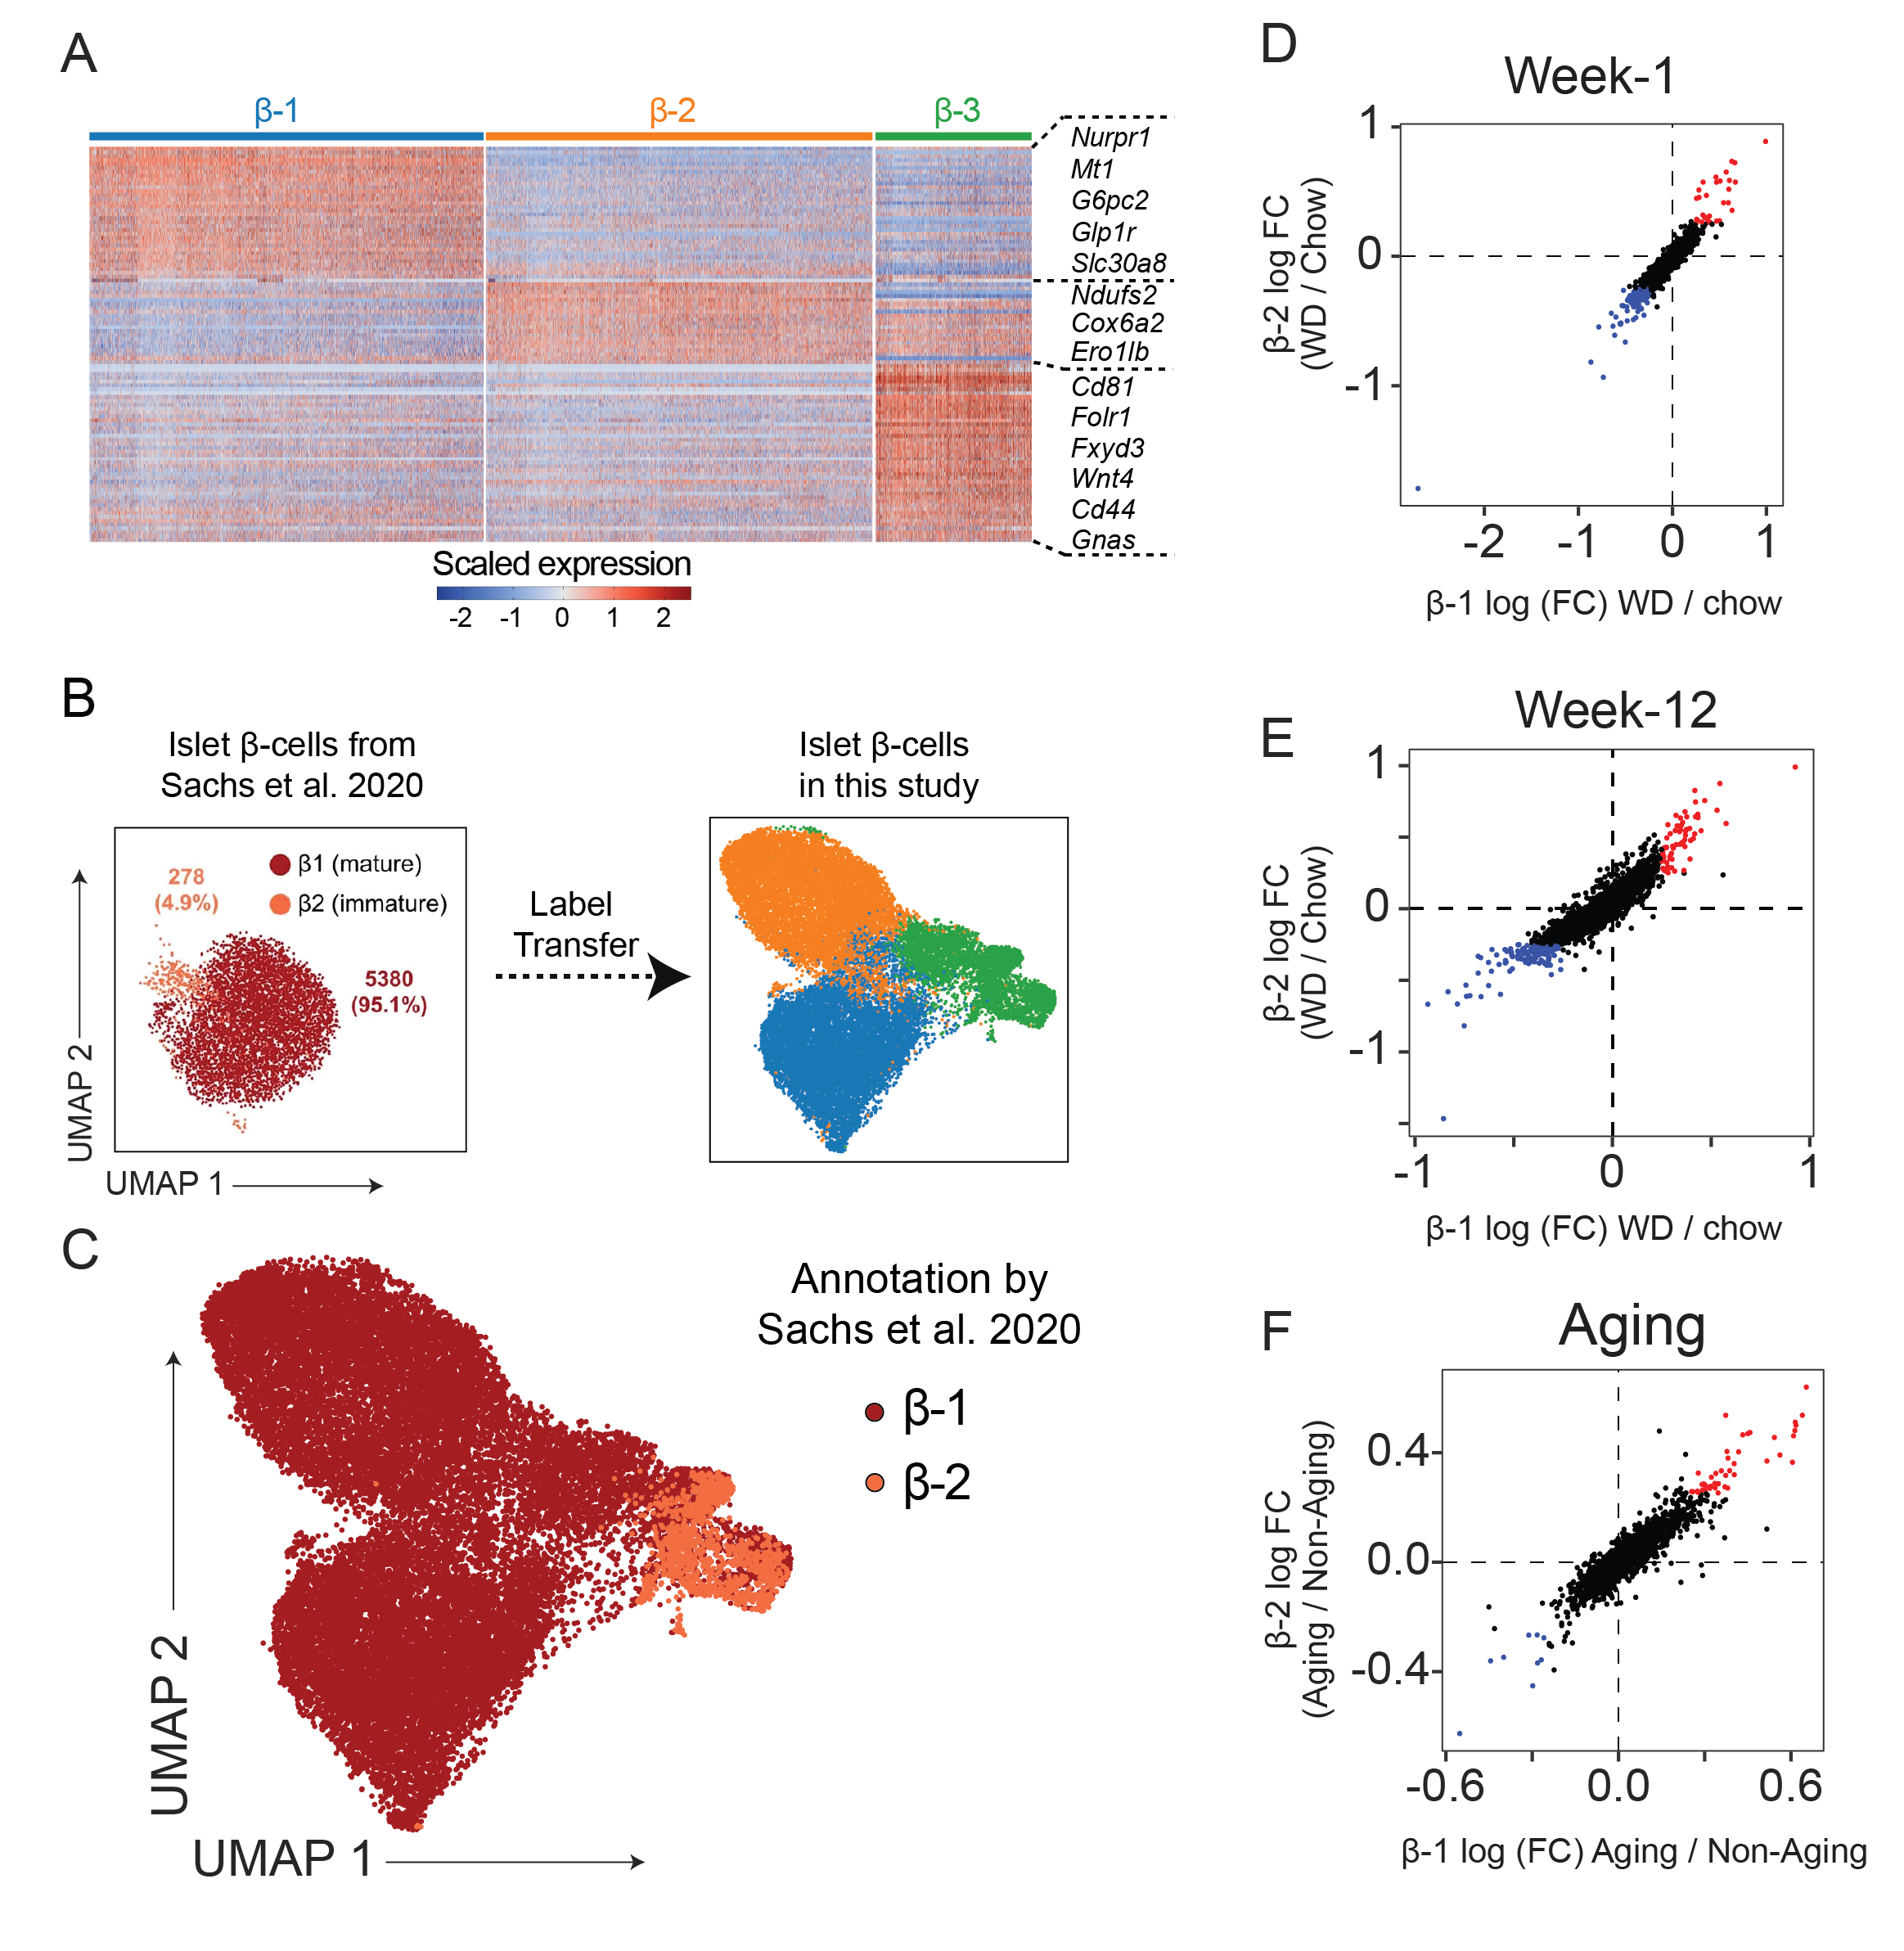
\includegraphics[width=\linewidth]{Appendix2/Fig/F2-12-03.png}
    \caption[Characterization of islet $\beta$-cells and their responses to \glslink{wd}{WD} and aging]{\textbf{Characterization of islet $\beta$-cells and their responses to \gls{wd} feeding and aging.} \textbf{(A)} Heatmap depicting scaled expression levels of marker genes in each $\beta$-cell sub-population from \textbf{\autoref{fig:chp2_scrna_betacells1} A}. \textbf{(B)} Schematic depicting the label transfer workflow to map the annotations of the $\beta$-cells from Sachs \textit{et al.} \textbf{\cite{sachs_targeted_2020}} onto the $\beta$-cells identified in this study. \textbf{(C)} \gls{umap} embedding of the islet $\beta$-cells from this study, grouped according to the annotations by Sachs \textit{et al.}  \textbf{\cite{sachs_targeted_2020}} following the label transfer workflow. \textbf{(D) - (F)} Scatter plots depicting the $\log$ \glsentrylong{fc} of \gls{de} genes in $\beta$-1 on x-axis and $\beta$-2 on y-axis for \gls{wd} versus chow diet after one week of feeding \textbf{(D)}, \gls{wd} versus chow diet after twelve weeks of feeding \textbf{(E)} and the aged mice versus non-aging controls (Week-1 + Week-12) \textbf{(F)}. The differentially up-regulated ($ Avg. \log \glslink{fc}{FC}  > 0.25 $)  and down-regulated ($ Avg. \log \glslink{fc}{FC} < -0.25 $) genes are indicated by red and blue dots respectively.}
    \label{fig:app_scrna_betacells1}
\end{figure}

\clearpage
%
\end{comment}

\begin{figure}[H]
    \centering
    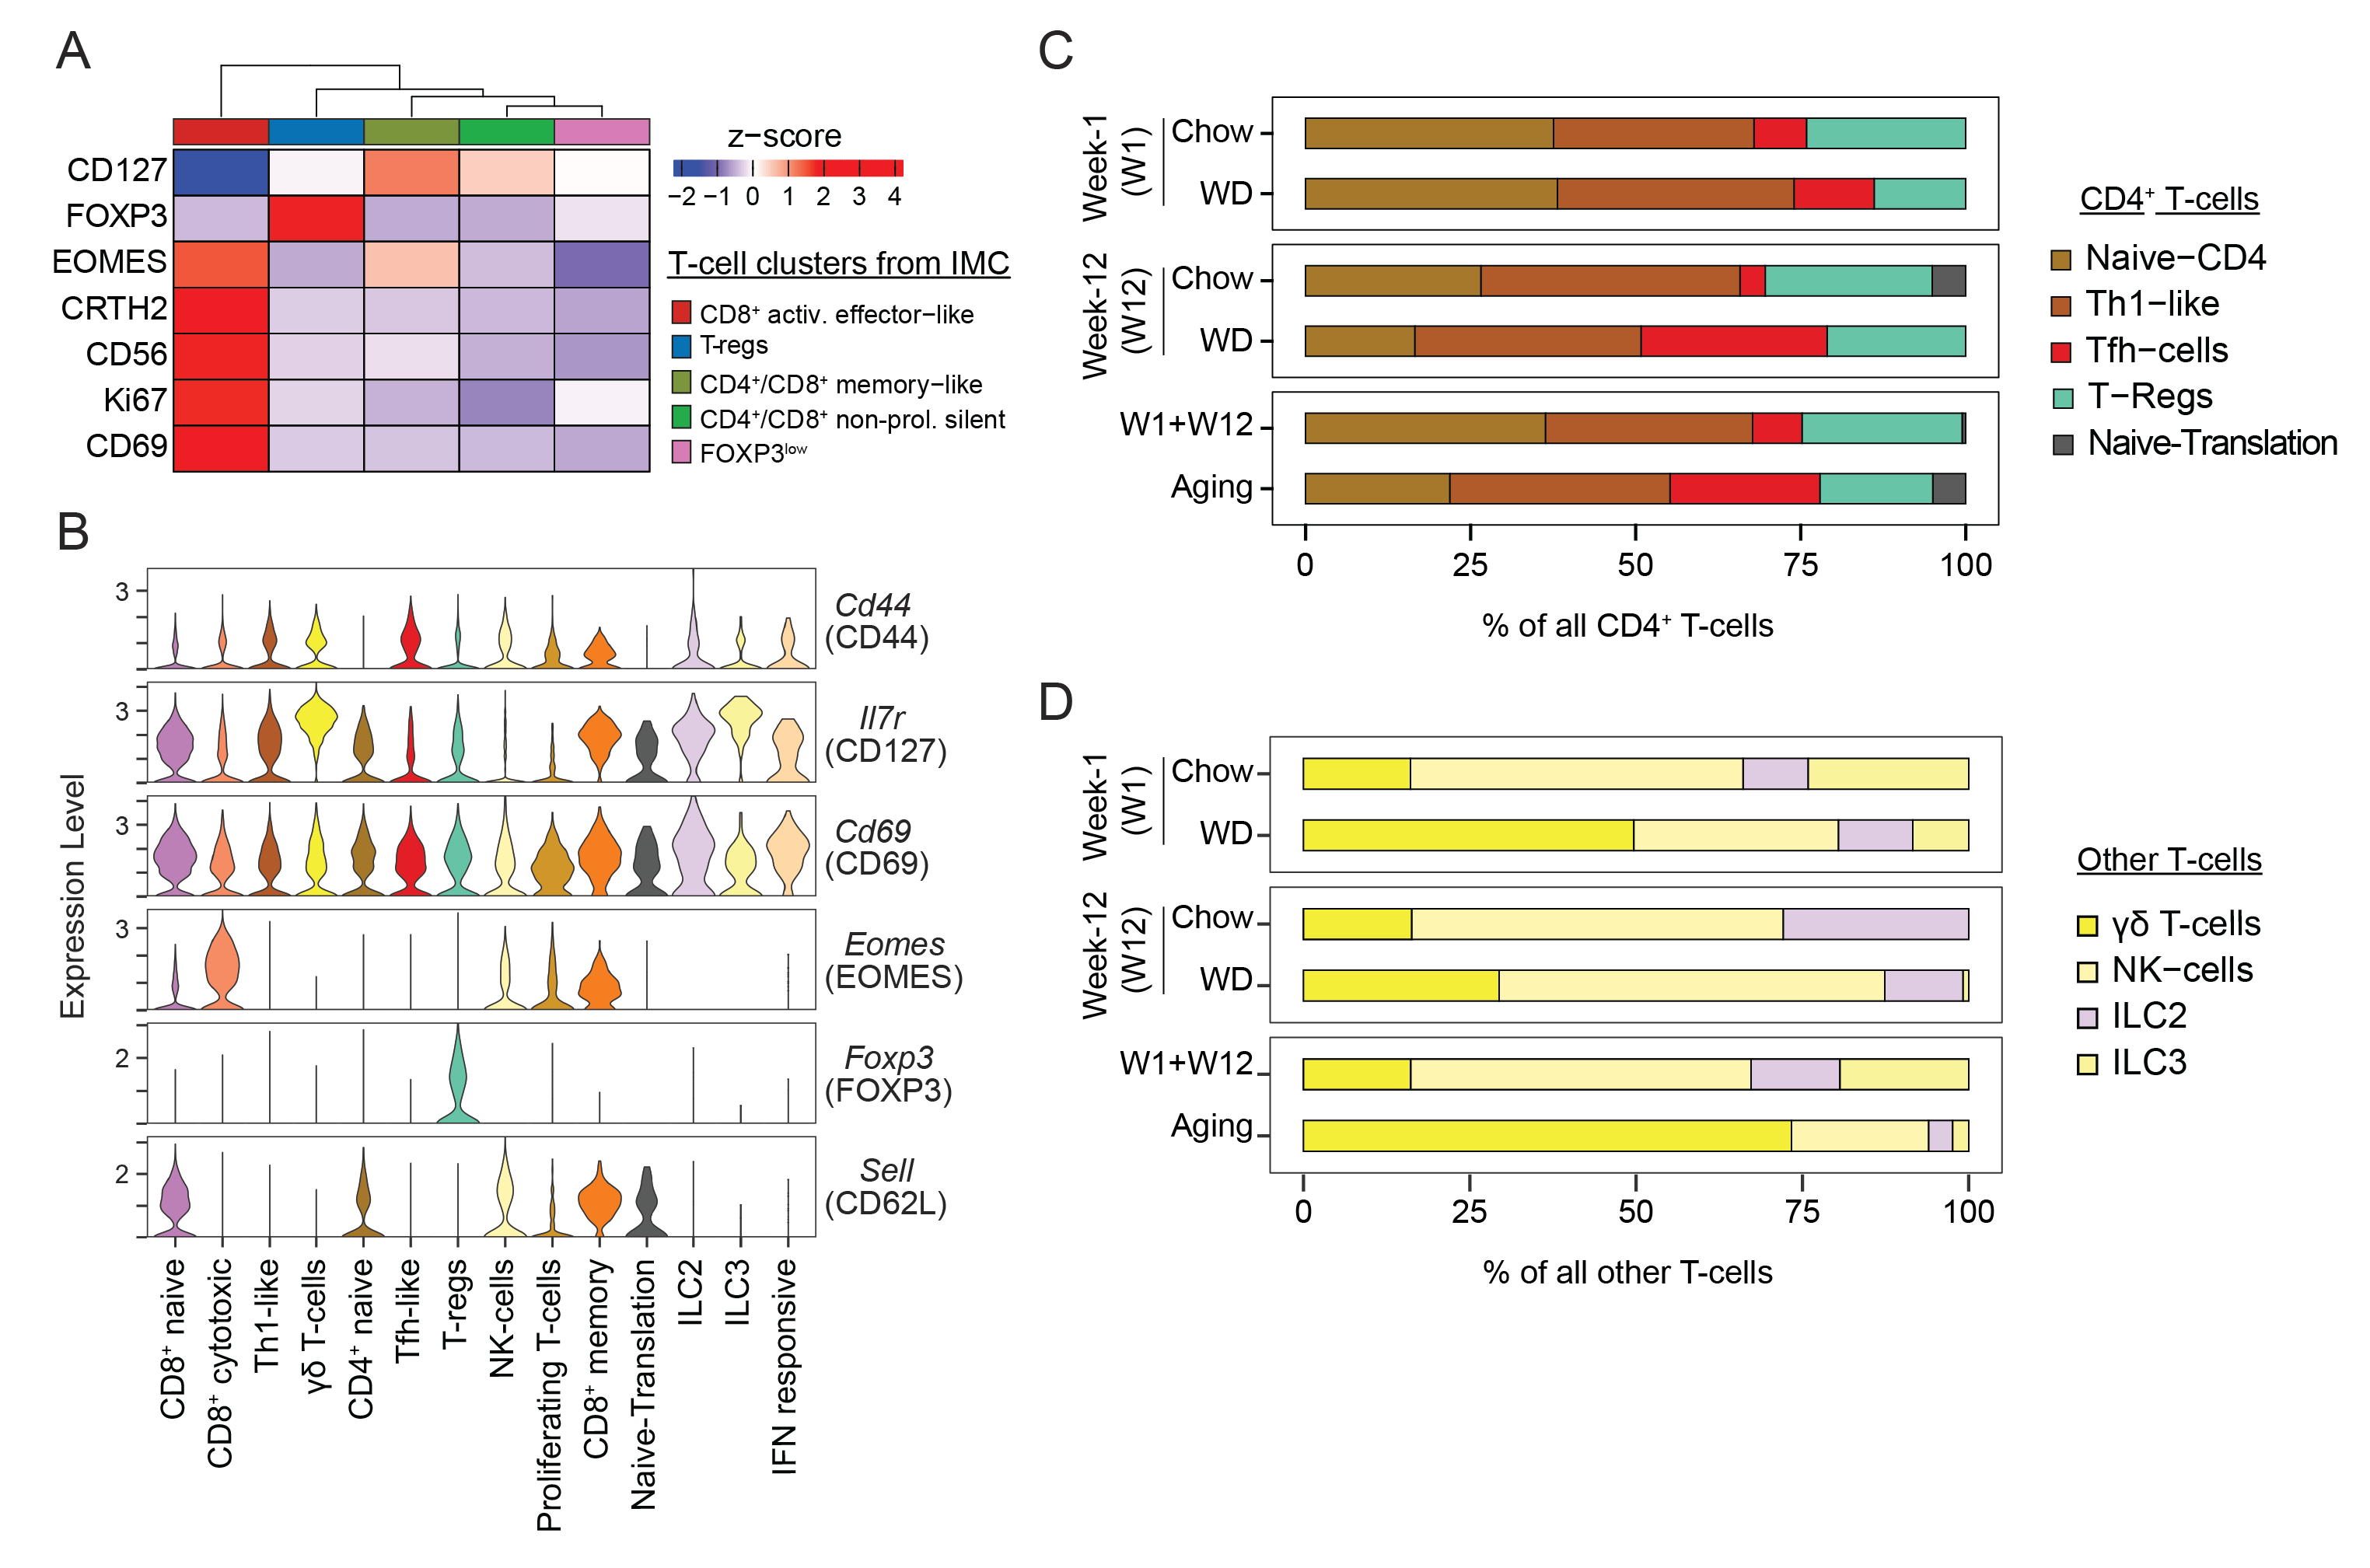
\includegraphics[width=\linewidth]{Appendix2/Fig/F2-A8-01.png}
    \caption[Linking T-cell sub-populations from \glsentryshort{scr} to \glsentryshort{imc}]{\textbf{Linking T-cell sub-populations from \gls{scr} to \gls{imc}.} \textbf{(A)} Heatmap depicting the \textit{z-score} expression of the indicated channels across five T-cell sub-populations identified in the \gls{imc} analysis. \textbf{(B)} Violin plots depicting the normalized expression of genes corresponding to indicated \gls{imc} channels in \textbf{(A)} across all T-cell sub-populations identified in the \gls{scr} analyis. \textbf{(C) - (D)} The proportion of each CD4+ T-cell sub-populations \textbf{(C)} and the other T-cell sub-populations \textbf{(D)}, computed as a percentage of all CD4+ cells and other T-cells respectively in every experimental group. The cells from different biological replicate cohorts were pooled together.}
    \label{fig:app_scrna_tcells1}
\end{figure}


\begin{figure}[H]
    \centering
    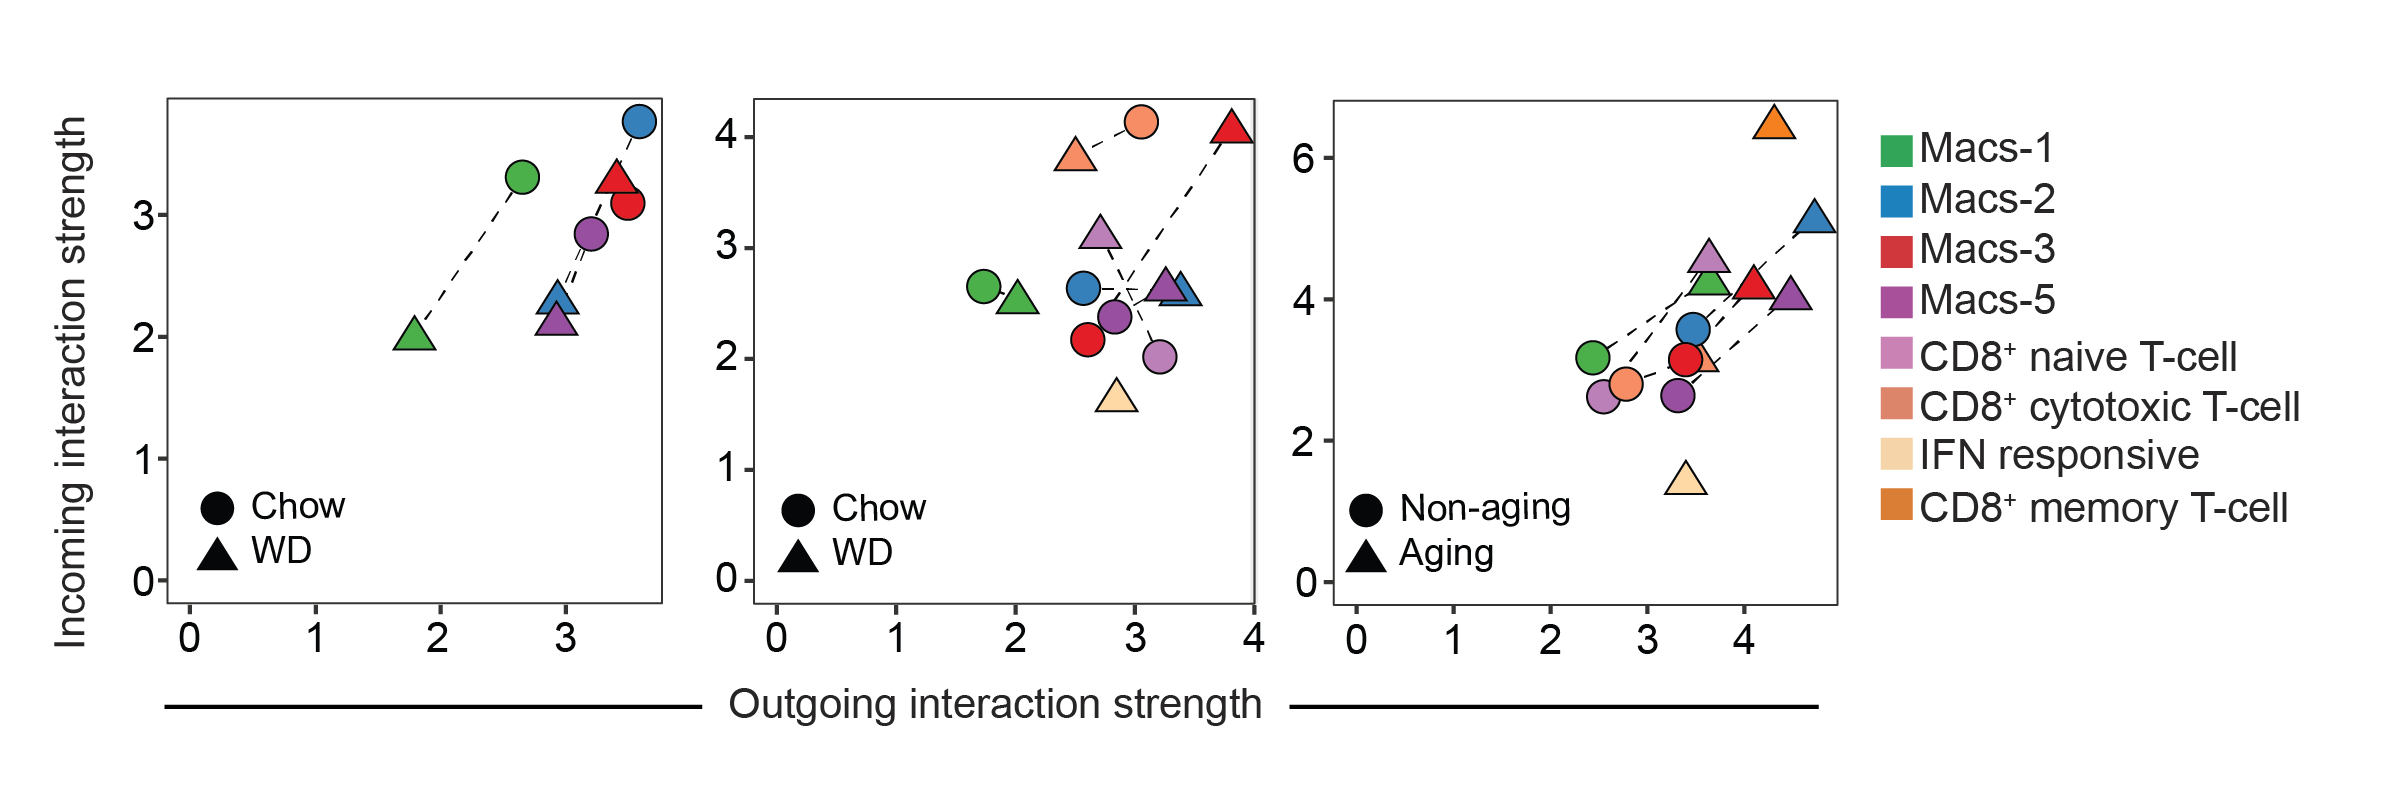
\includegraphics[width=\linewidth]{Appendix2/Fig/F2-A1-v3-01.png}
    \caption[\glsentryshort{lri} analysis in macrophage and T-cell sub-populations]{\textbf{\gls{lri} analysis in macrophage and T-cell sub-populations.} Scatter plot depicting the outgoing and the incoming interaction strength for the non-proliferating macrophage and CD8\textsuperscript{+} T-cell sub-populations at Week-1 (left), Weeks-12 (middle) and Aging (right) time-points. The Non-aging group is comprised of Week-1 and Week-12 chow diet cohorts.}
    \label{fig:app_scrna_cellchat1}
\end{figure}

% - (D) \textbf{(C)} and from Macs-3 to CD8\textsuperscript{+}  cytotoxic T-cells \textbf{(D)} 


% \begin{figure}[!t]
%     \centering
%     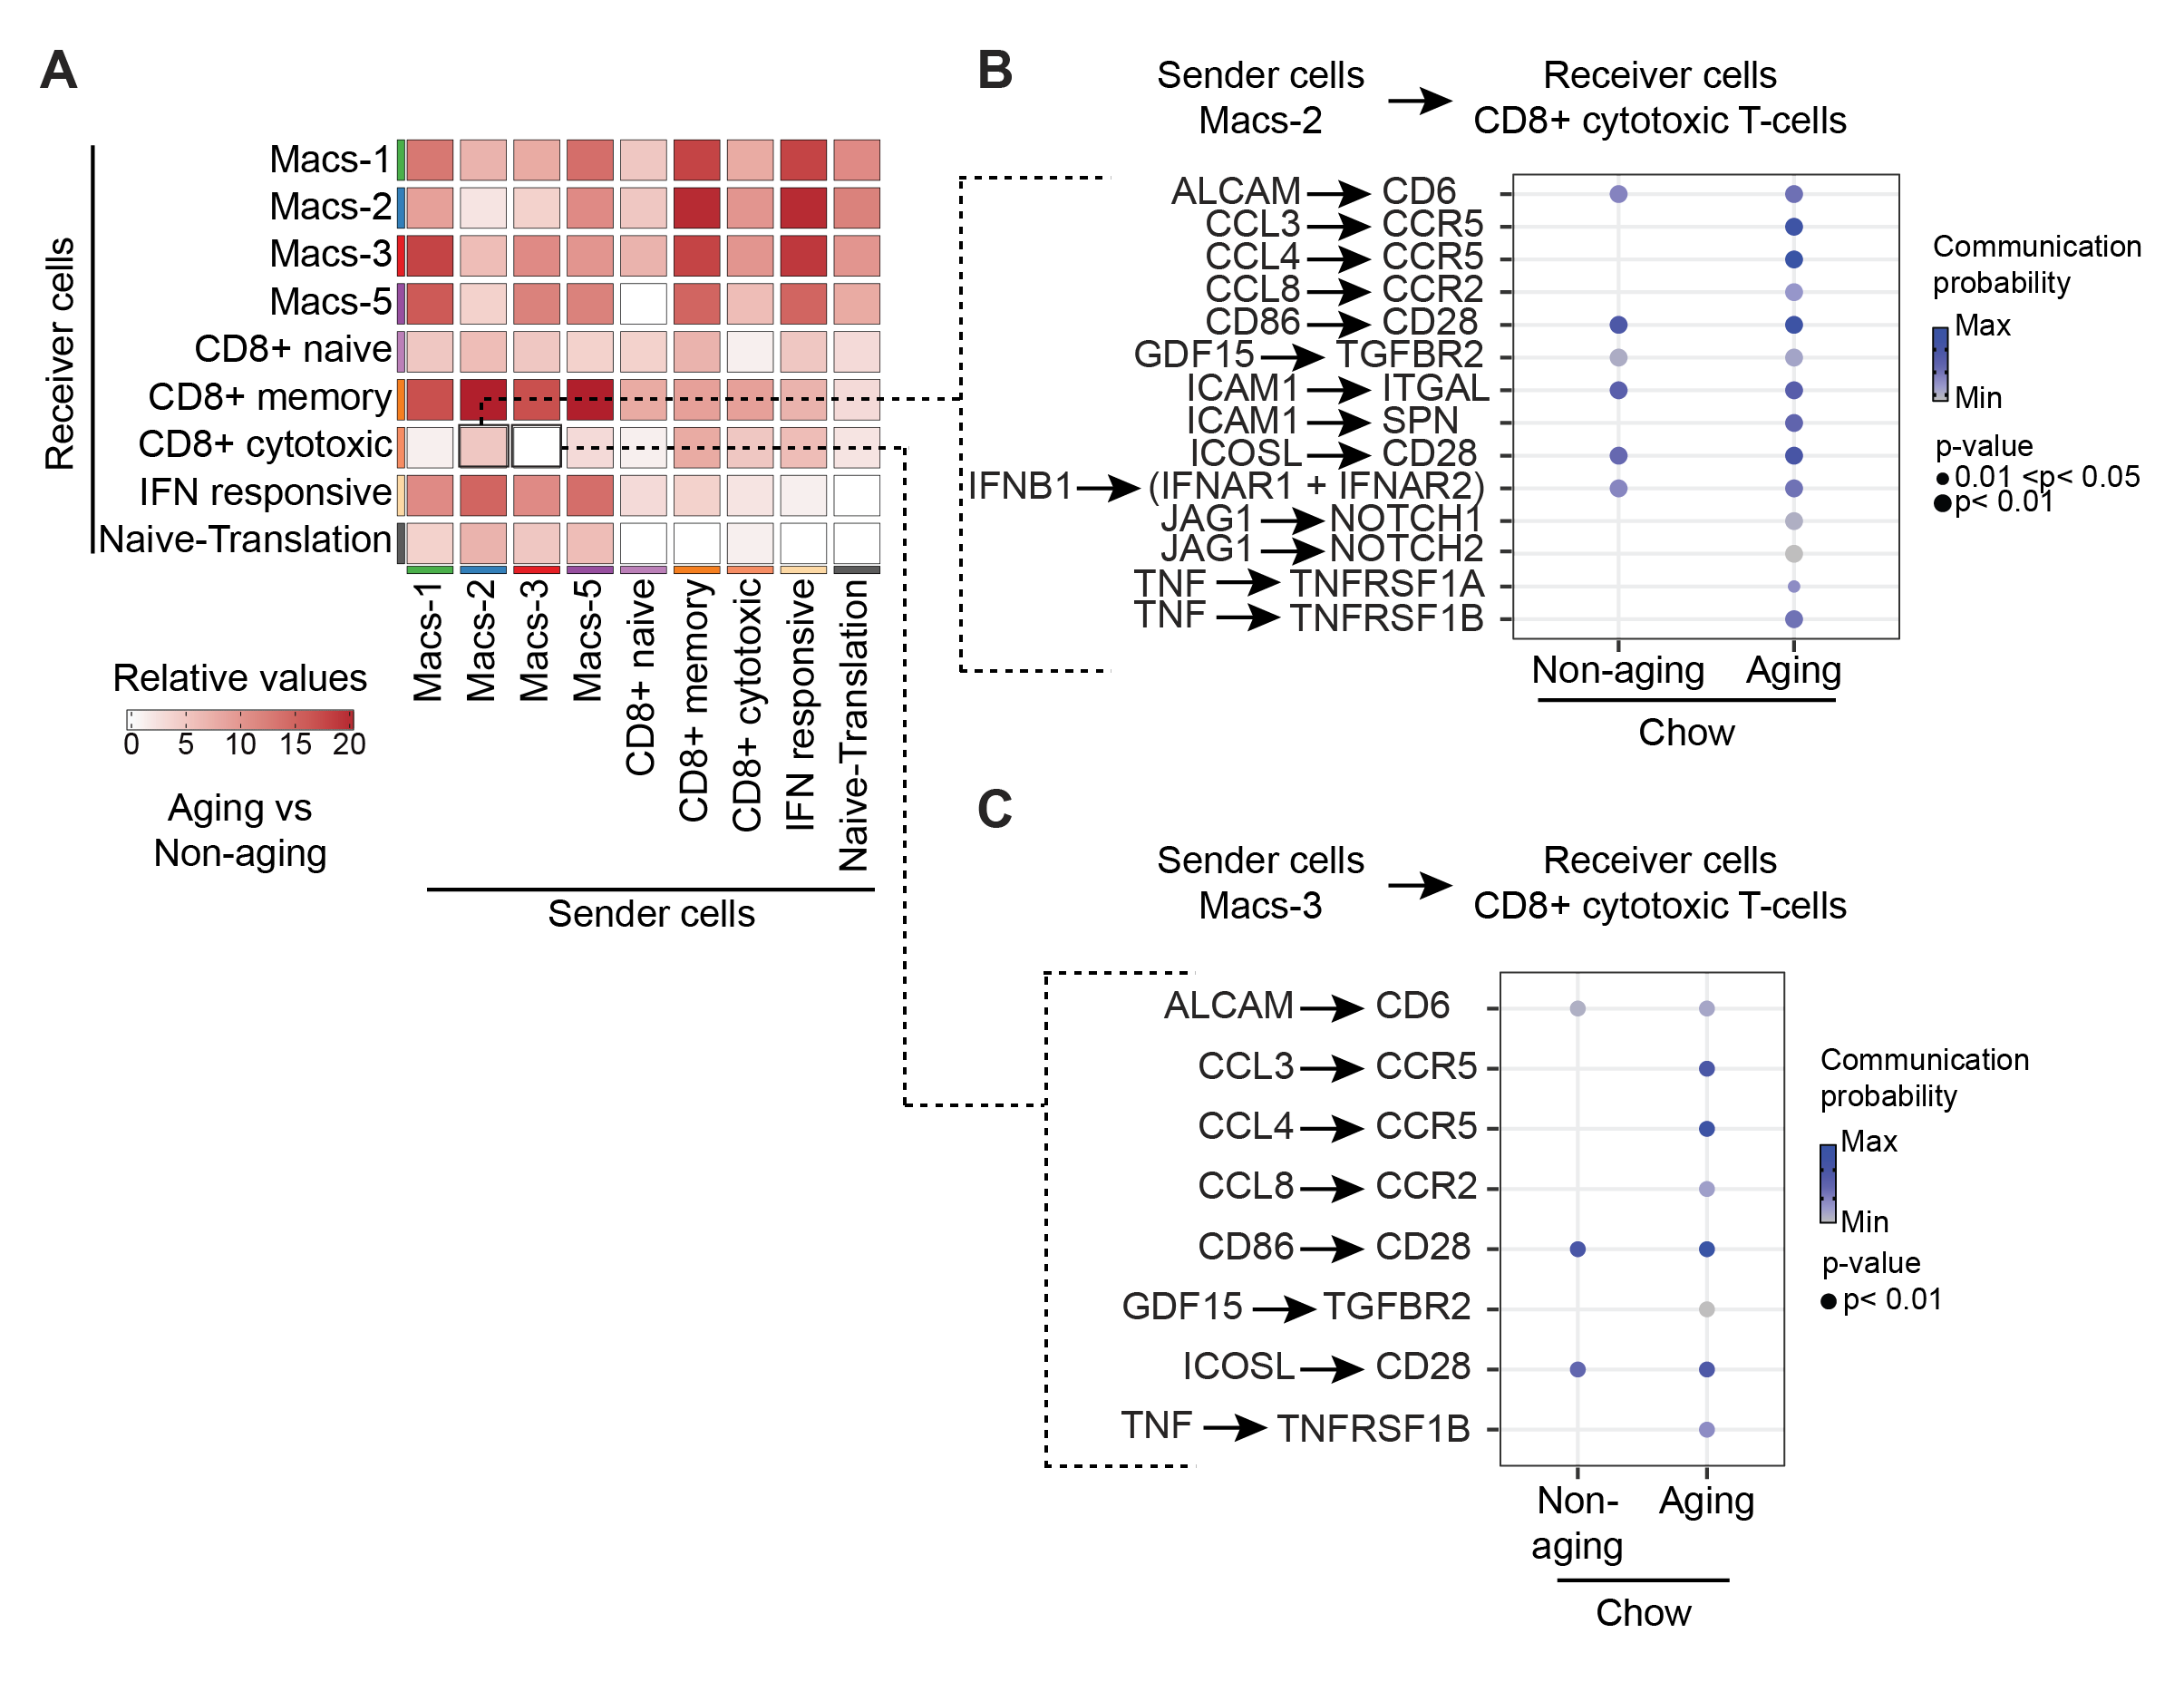
\includegraphics[width=\linewidth]{Appendix2/Fig/F2-A1-02.png}
%     \caption[Differential interaction analysis between chow-fed aging and chow-fed non-aging (Week-1 and Weeks-12) groups]{\textbf{Differential interaction analysis between chow-fed aging and chow-fed non-aging (Week-1 and Weeks-12) groups}\\\\
%     \textbf{(A)} Heatmap depicting differential number of interactions in the Aging cohort (n = 2) compared to the Non-Aging (Week-1 Chow (n=3) and Week-12 Chow (n=3)) cohorts between the indicated cell populations. \textbf{(B)}Dot plots depicting ligand-receptor interaction intensity, with signals from Macs-2 to CD8+ cytotoxic, under Chow (n=3) and one-week post-Western diet (n=2) conditions. The plots specifically highlight signals that exhibit an increase in interaction intensity from non-aging to aging condition. The dot color and size represent the calculated communication probability and p-values. p-values are computed from one-sided permutation test directly within CellChat. \textbf{(C)} Dot plots depicting ligand-receptor interaction intensity, with signals from Macs-3 to CD8+ cytotoxic, under Chow (n=3) and one-week post-Western diet (n=2) conditions. The plots specifically highlight signals that exhibit an increase in interaction intensity from non-aging to aging condition. The dot color and size represent the calculated communication probability and p-values. p-values are computed from one-sided permutation test directly within CellChat.}
%     \label{suppl_fig:cell_cell2}
% \end{figure}




\clearpage

%\begin{comment}
    

\section[\autoref{chp:meta_analysis}]{Additional results for \autoref{chp:meta_analysis}}

\begin{figure}[H]
\centering
\vspace{-30pt}
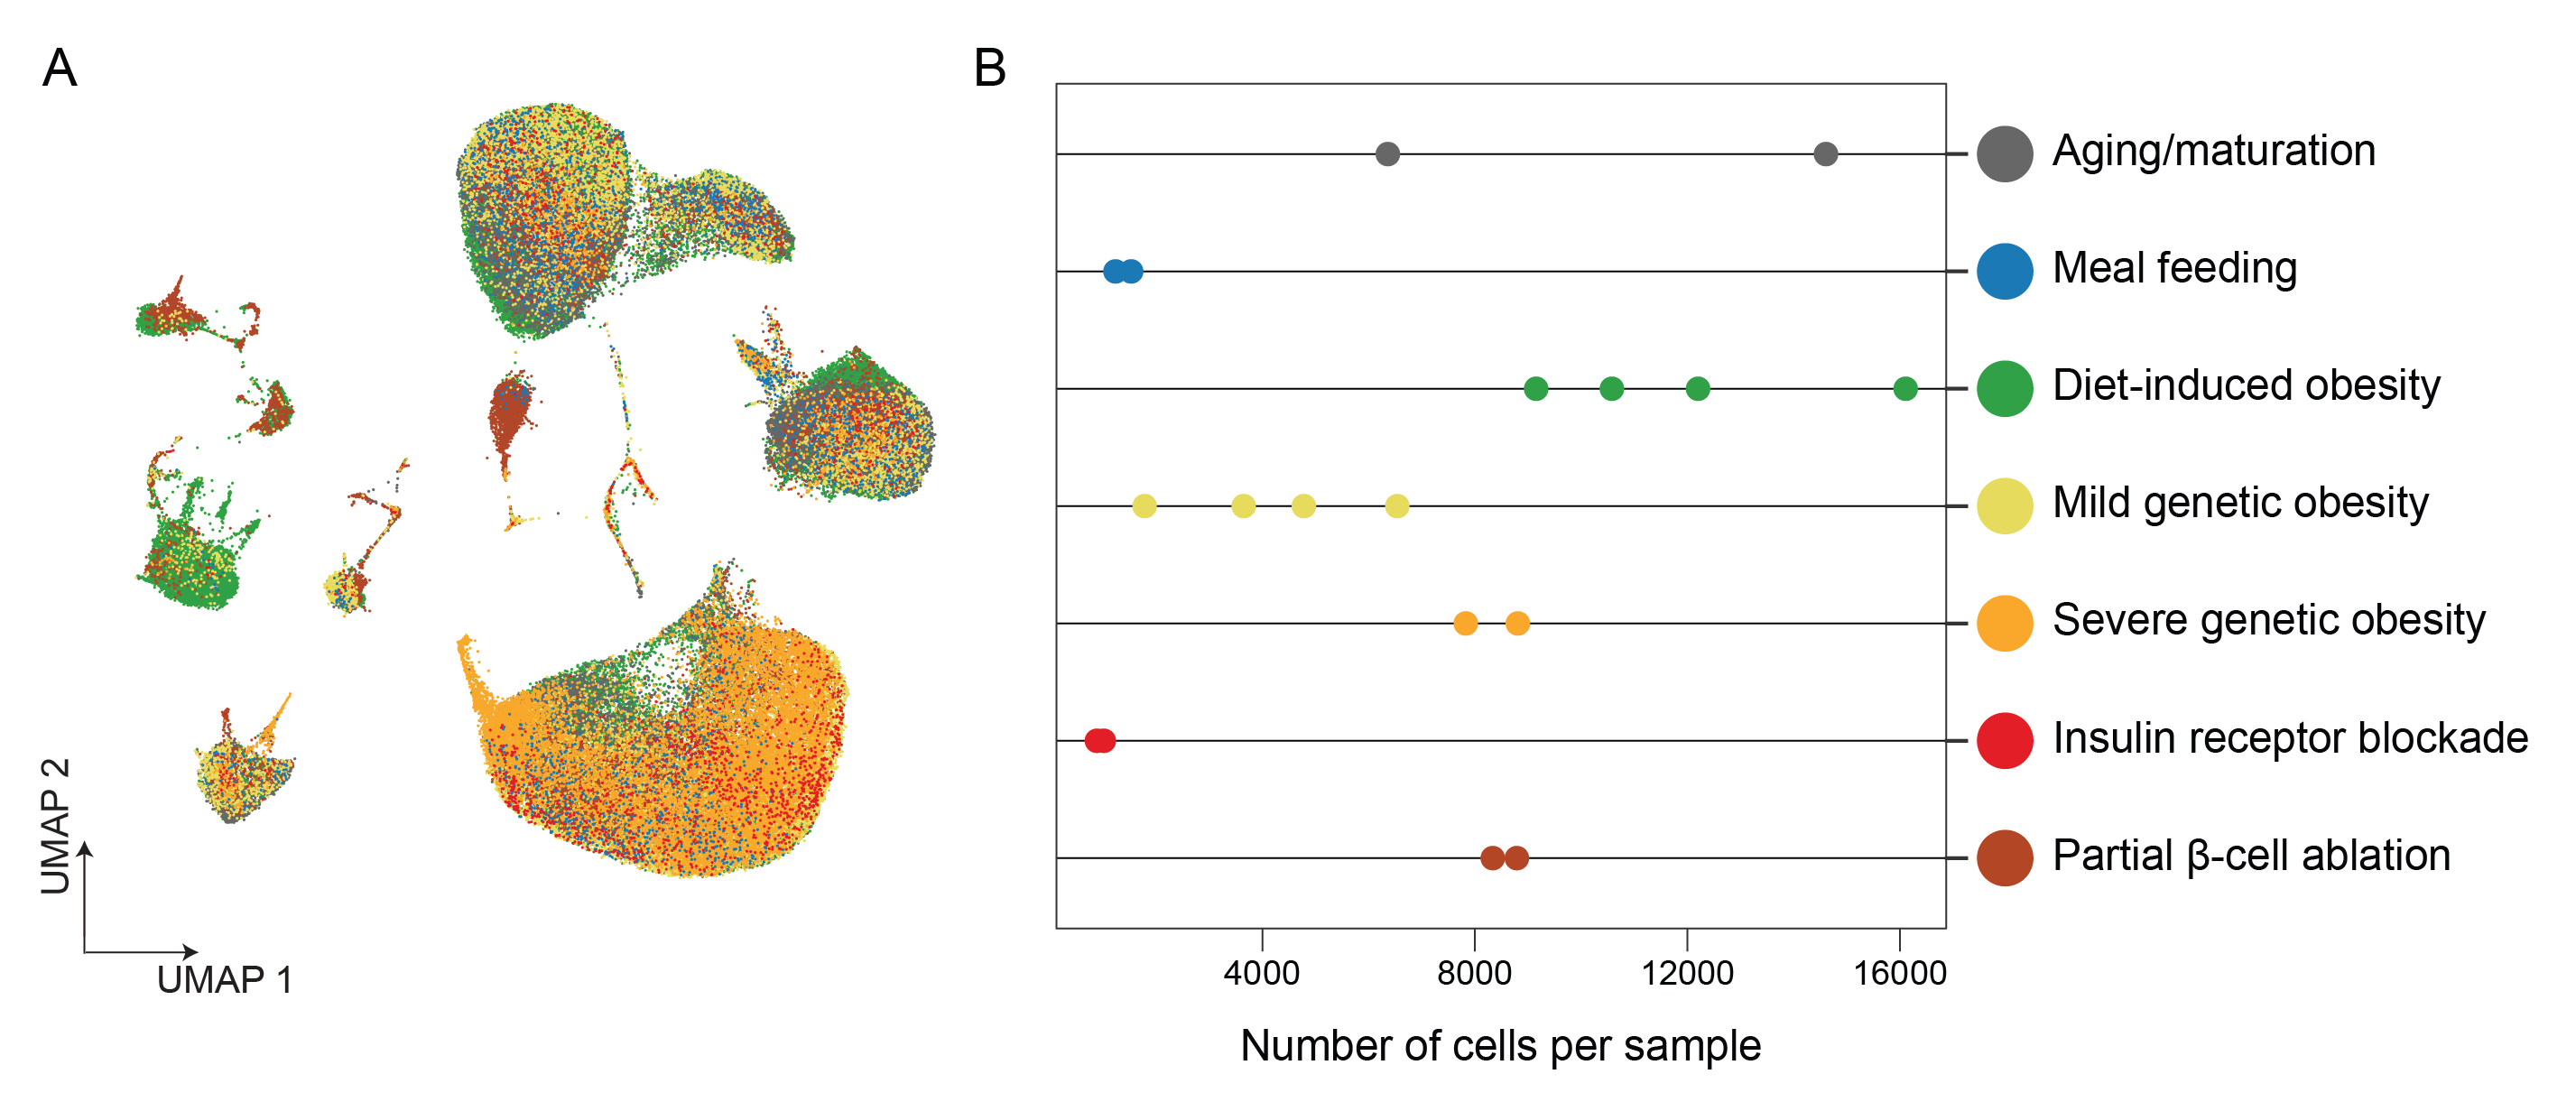
\includegraphics[width=\linewidth]{Appendix2/Fig/F3-2-v2-02.png}
\caption[Study distribution in the full integrated data]{\textbf{Study distribution in the full integrated data.} \textbf{(A)} \gls{umap} embedding of the full integrated dataset depicting the seven studies Incorporated into this atlas. \textbf{(B)} Number of cells after \gls{qc} per group within each study included in this atlas. Metadata about the individual studies can be found in \textbf{\autoref{tab:app_chp3_study}} and the number of cells per experimental sample can be found in \textbf{\autoref{tab:app_chp3_cellnumbers}}.}
\label{fig:app_chp3_study}
\end{figure}
\vspace{-22pt}

% \begin{figure}[H]
% \centering
% 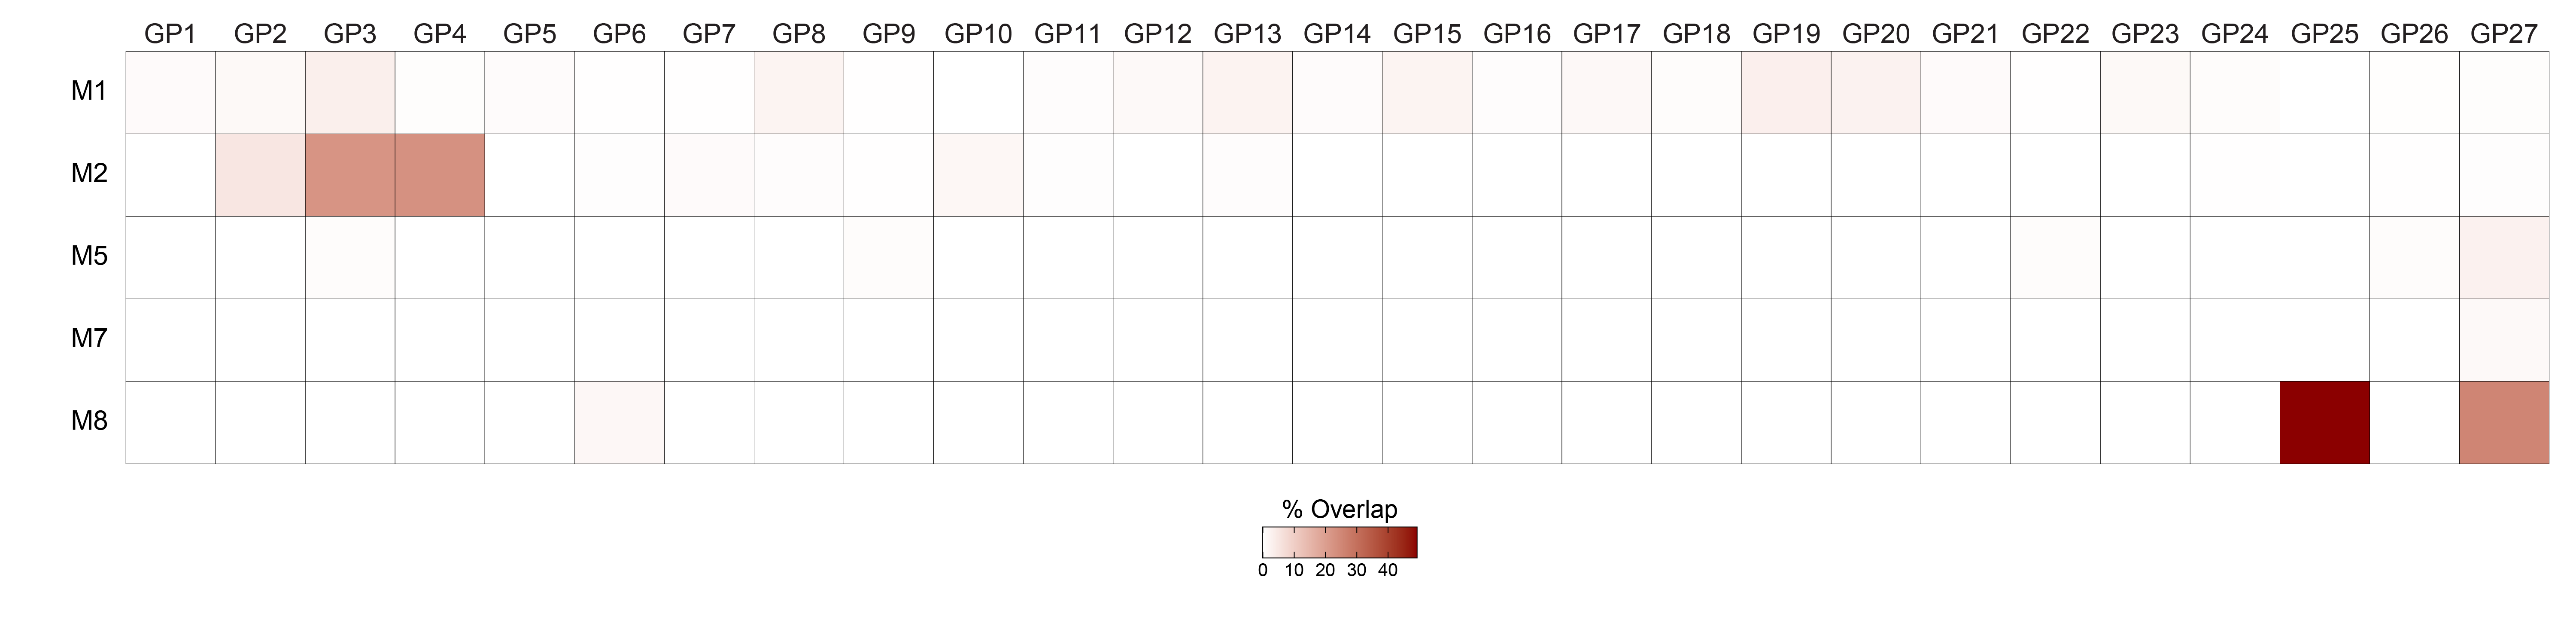
\includegraphics[width=\linewidth]{Appendix2/Fig/F3-5-01.png}
% \caption[Overlap between gene modules identified in this study and gene programs from MIA]{\textbf{Overlap between gene modules identified in this study and gene programs from MIA}}
% \label{suppl_fig:chp3_overlap}
% \end{figure}

\begin{figure}[H]
\centering
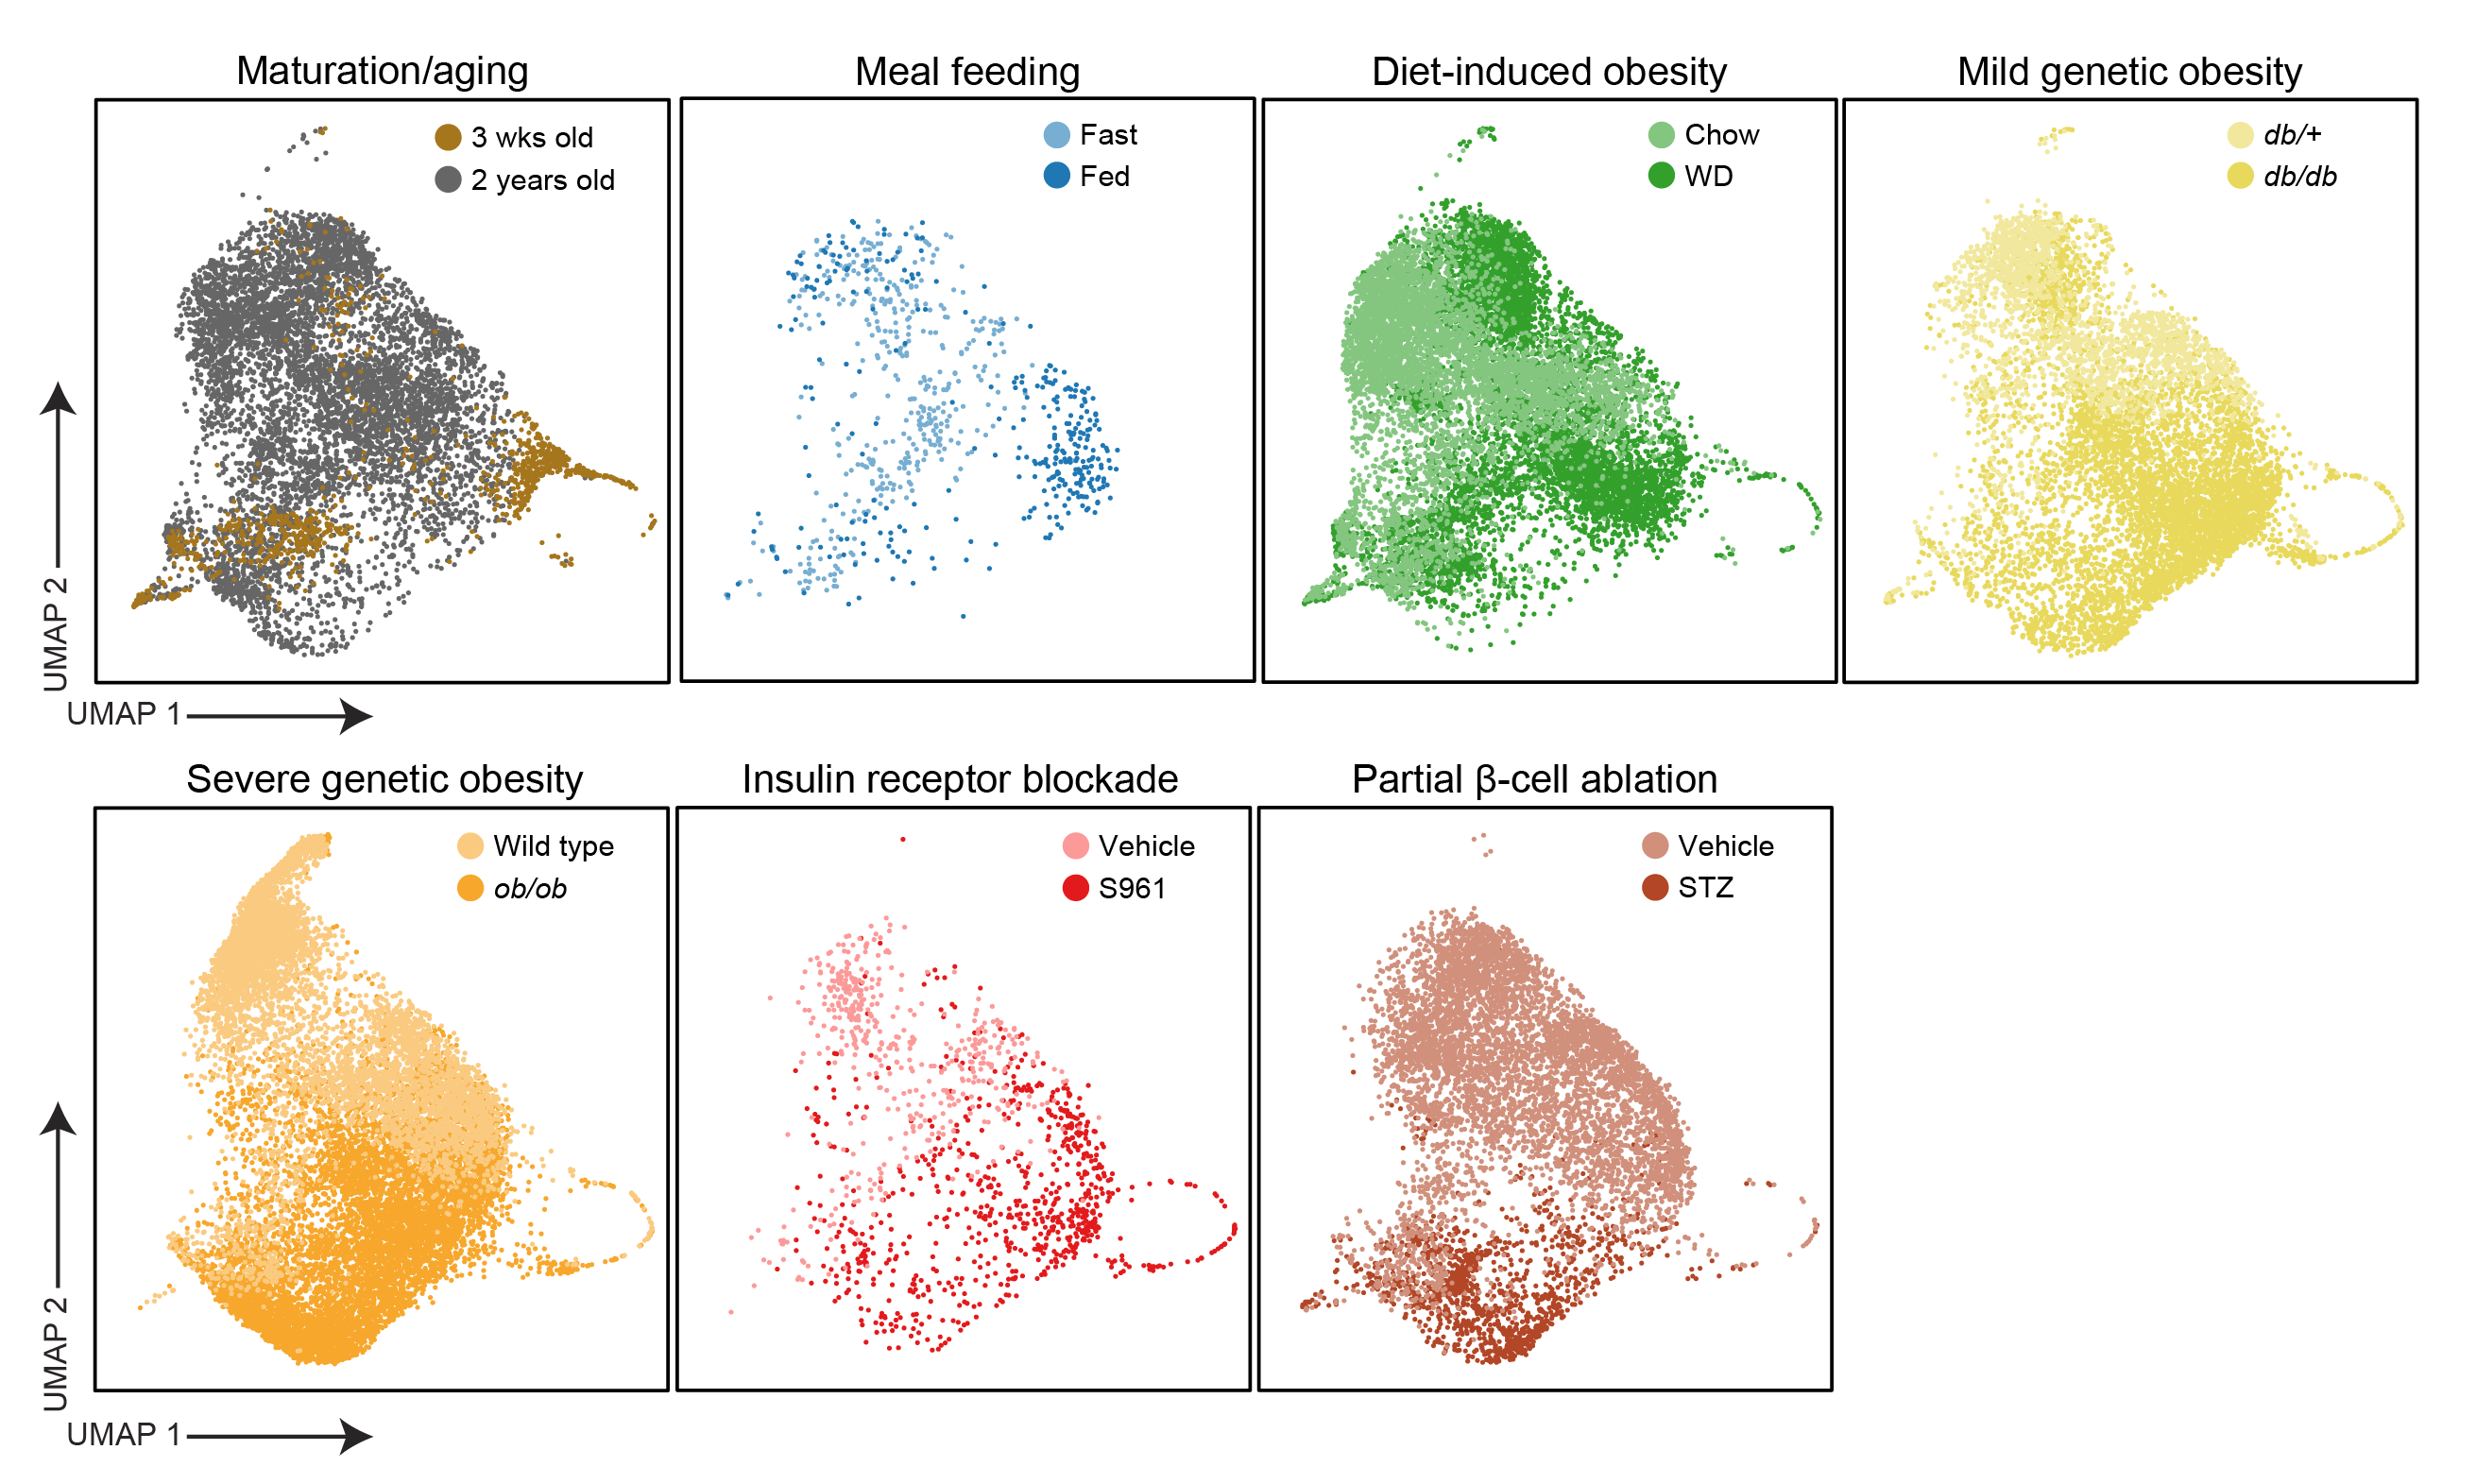
\includegraphics[width=\linewidth]{Appendix2/Fig/F3-4-01.png}
\caption[Split view of the integrated $\beta$-cell subset across seven studies]{\textbf{Split view of the integrated $\beta$-cell subset across seven studies.} \gls{umap} embedding of the re-integrated $\beta$-cell subset split across the seven studies included in this atlas. Within each dataset, $\beta$-cells are grouped according to healthy control and the corresponding experimental sample. The diet/induced obesity and the mild genetic obesity models have two time-points per group. Metadata about the individual studies can be found in \textbf{\autoref{tab:app_chp3_study}} and the number of cells per experimental sample can be found in \textbf{\autoref{tab:app_chp3_cellnumbers}}.}
\label{fig:app_chp3_betastudy}
\end{figure}



% \begin{figure}[H]
% \centering
% 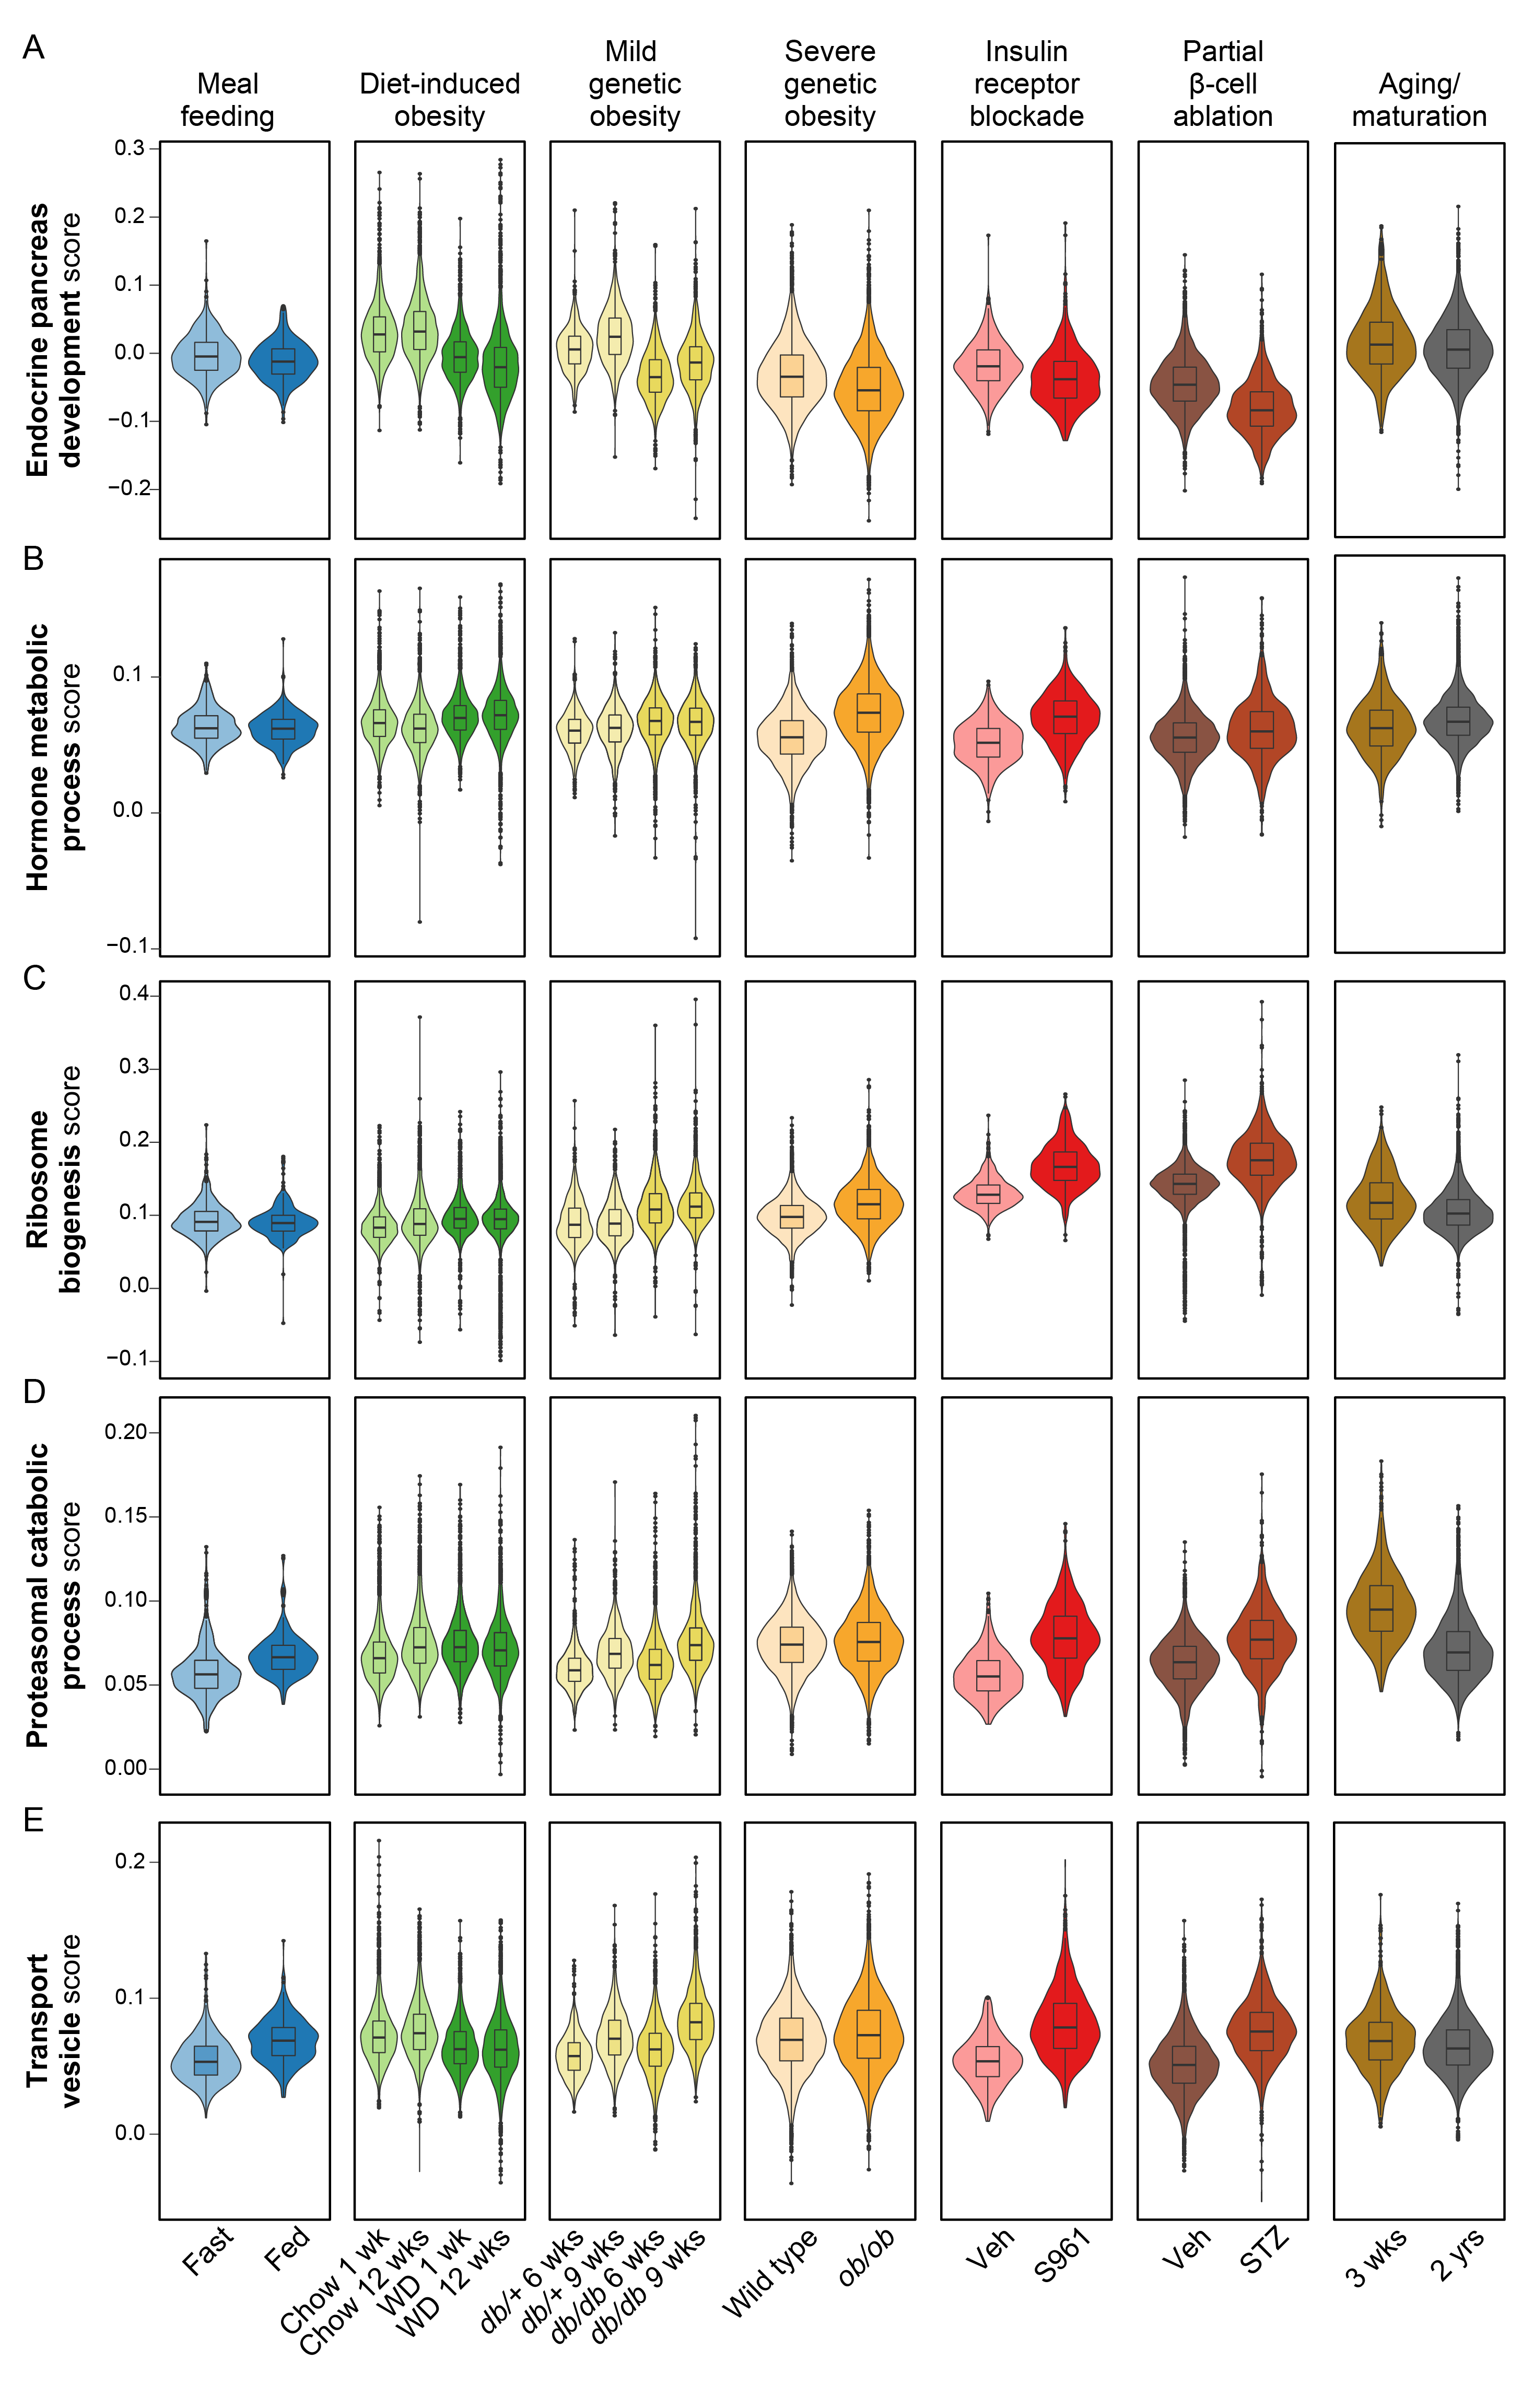
\includegraphics[width=12cm,height=keepaspectratio]{Appendix2/Fig/F3-21-01.png}
% \caption[]{\textbf{Helloellelelalaslls}}
% \label{fig:app_chp3_humant2d}
% \end{figure}

\begin{SCfigure}[][h]
  \centering
  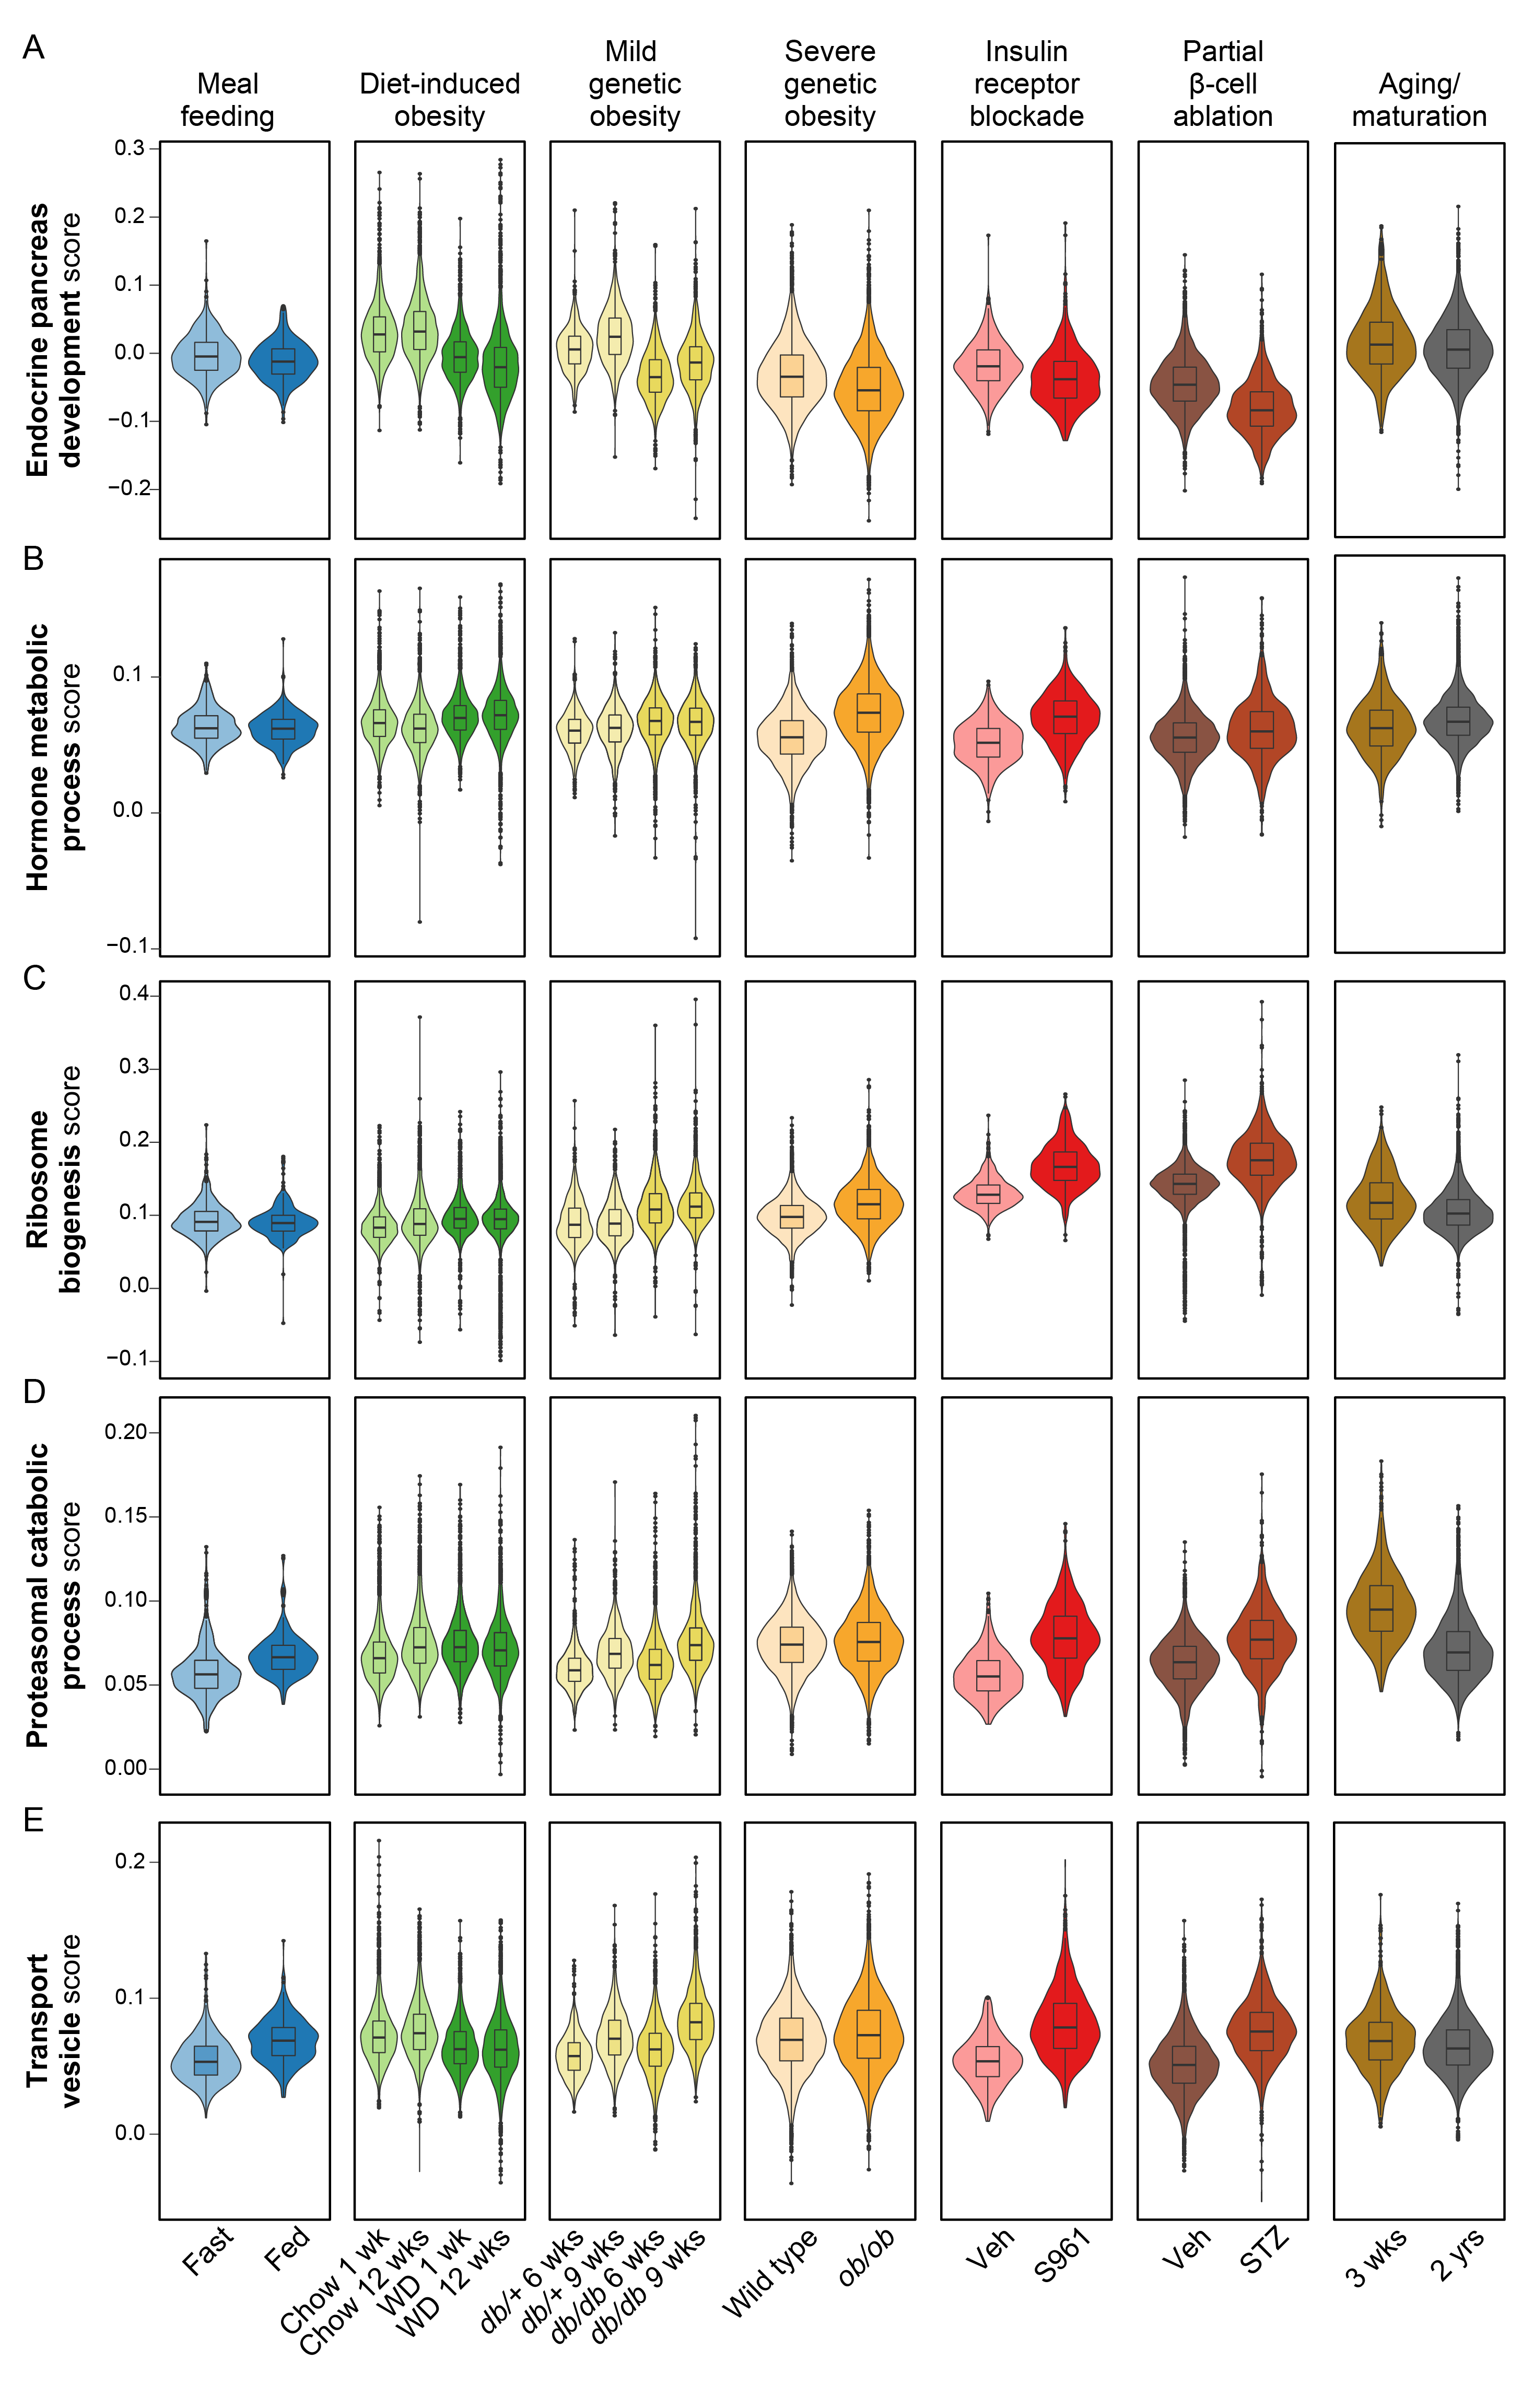
\includegraphics[width=0.6\linewidth]{Appendix2/Fig/F3-21-01.png}
  \vspace{-150pt}
  \caption[Module scoring of human up-regulated \glsentryshort{t2d} gene sets]{\textbf{Module scoring of human up-regulated \gls{t2d} gene sets.} \textbf{(A) - (E)} Violin plots depicting the gene set scores for Endocrine pancreas development \textbf{(A)}, Hormone metabolic process \textbf{(B)}, Ribosome biogenesis \textbf{(C)}, Proteasomal catabolic process \textbf{(D)} and Transport vesicle \textbf{(E)} associated genes shown for $\beta$-cell workload models and corresponding healthy controls from individual studies. On the overlay box plots, the middle horizontal line represents the median, the box represents the inter-quartile range and the whiskers represent the minimum and maximum values. The number of cells are indicated in \textbf{\autoref{tab:app_chp3_cellnumbers}}.}
  \label{fig:app_chp3_humant2d}
\end{SCfigure}




\begin{figure}[H]
\centering
\vspace{150pt}
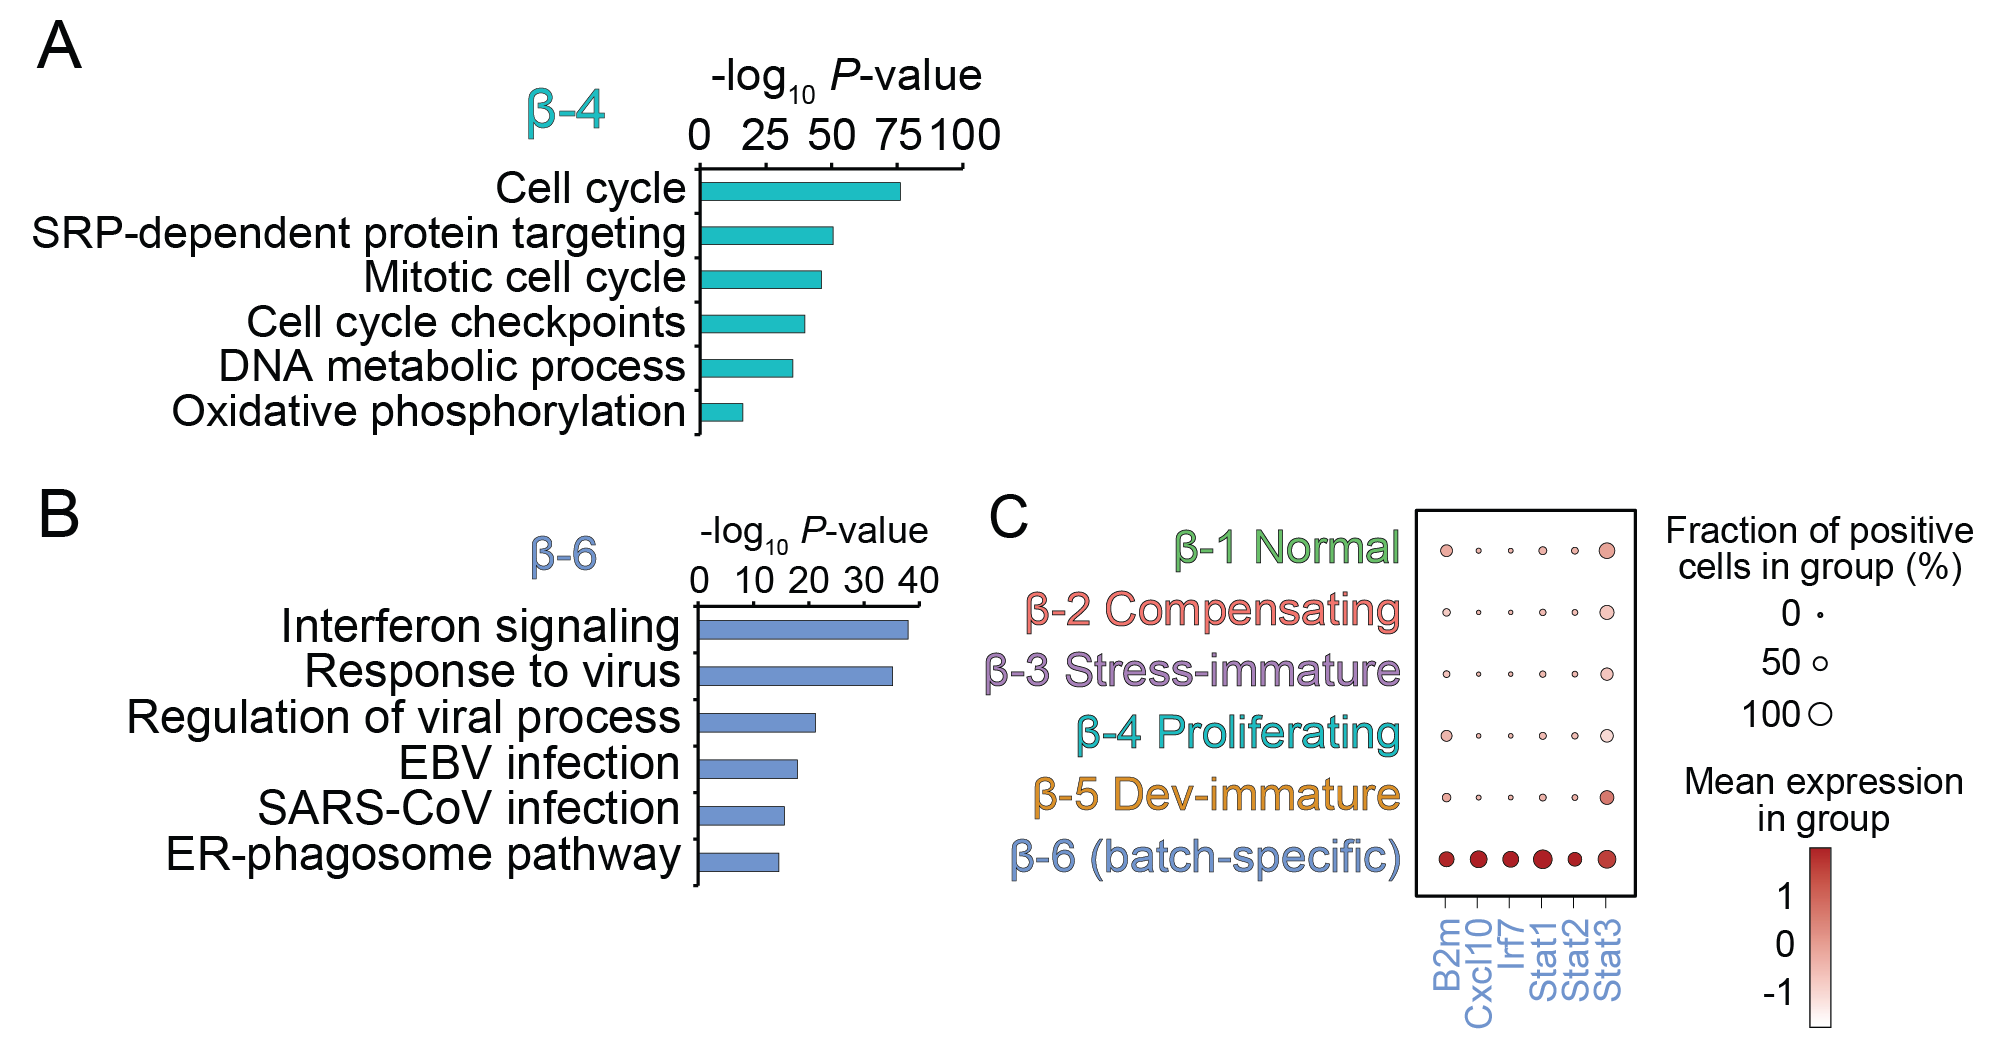
\includegraphics[width=\linewidth]{Appendix2/Fig/F3-1-v2-01.png}
\caption[Characterization of $\beta$-cell subsets]{\textbf{Characterization of $\beta$-cell subsets}. \textbf{(A) - (B)} Bar plots depicting enriched \gls{go} terms for $\beta$-4  and $\beta$-6 subsets. The significance ($-\log_{10}$ p-value) of the enrichment are shown. No enriched terms were found for $\beta$-5 subset. \textbf{(C)} Dot plot of the indicated genes highly expressed in $\beta$-6 subset. The color of the dots represent the scaled average expression and the size of the dots correspond to the percentage of cells expressing the given marker genes.}
\label{fig:app_chp3_betasubsets}
\end{figure}
%\vspace{-27pt}

% \begin{figure}[H]
% \centering
% 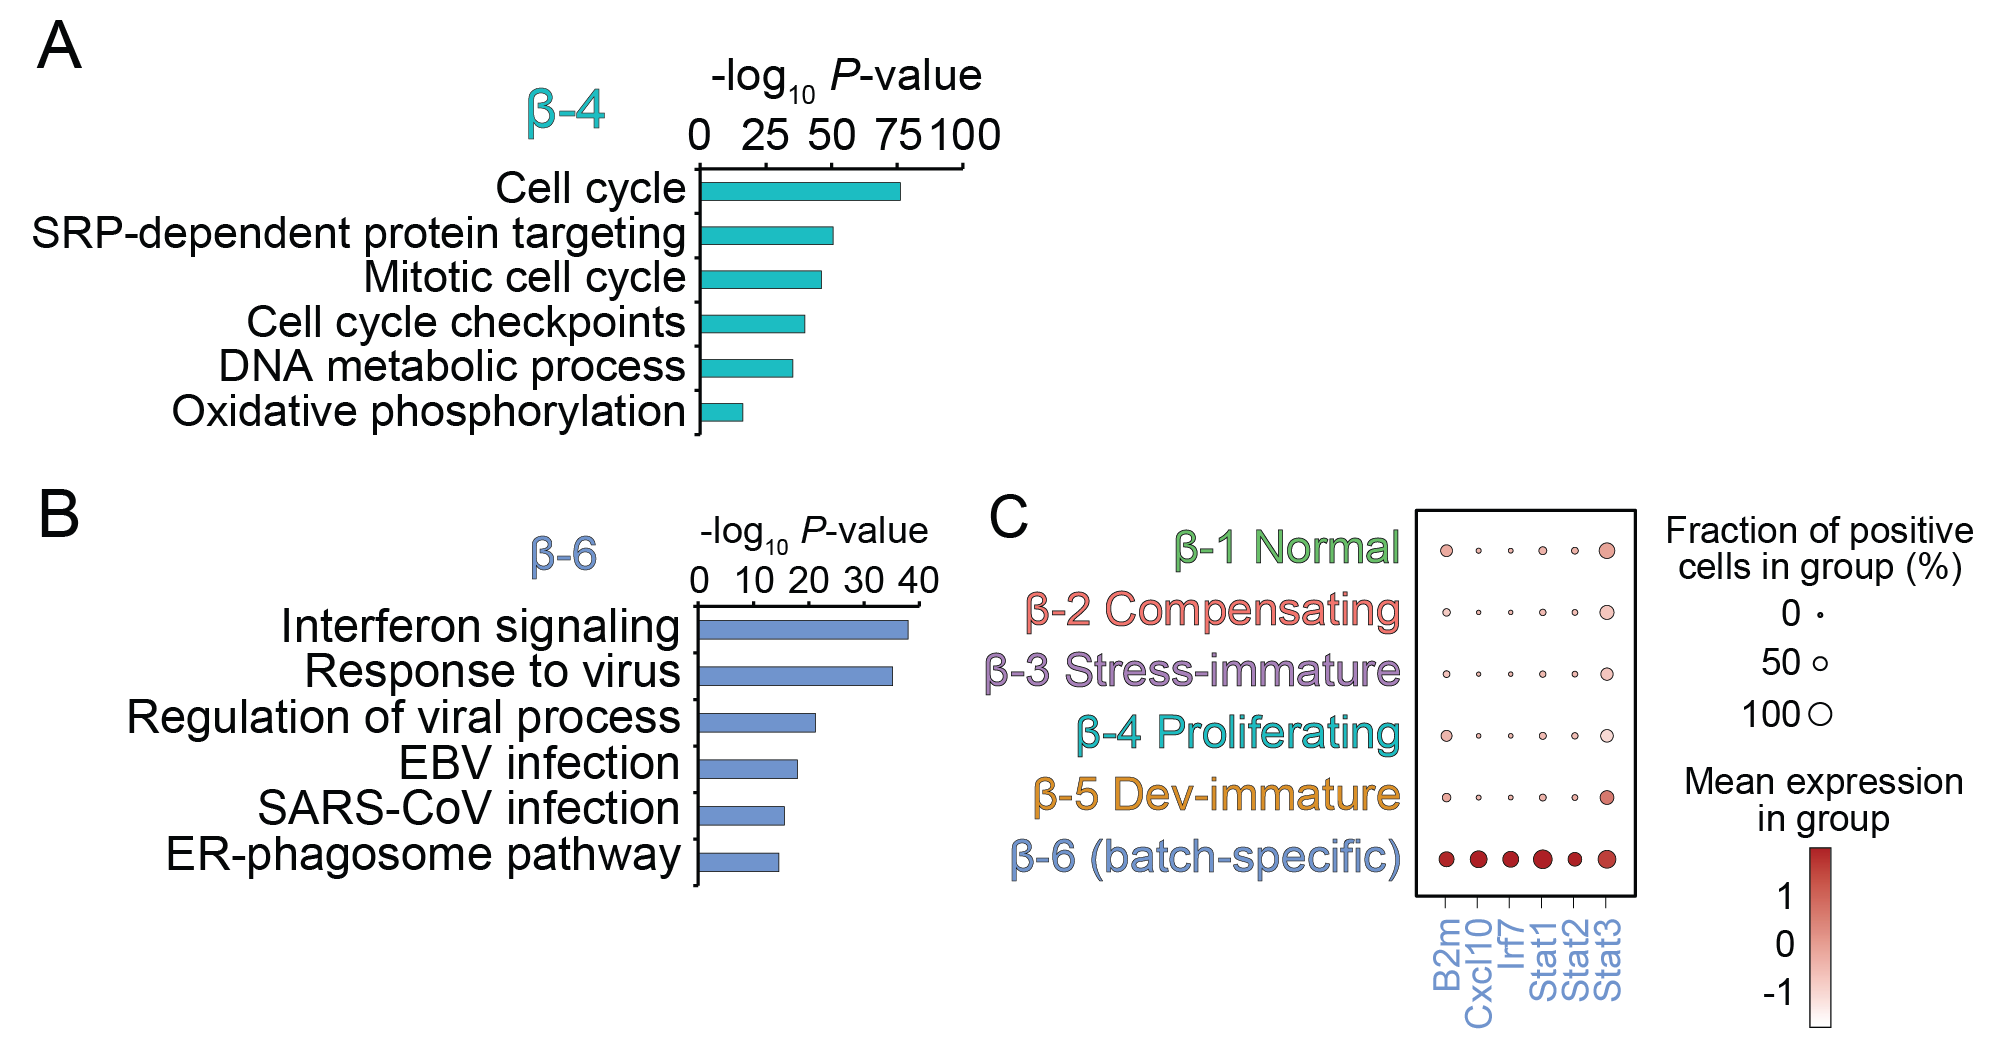
\includegraphics[width=\linewidth]{Appendix2/Fig/F3-1-v2-01.png}
% \caption[Characterization of $\beta$-cell subsets using enriched markers and gene ontology]{}
% \label{suppl_fig:chp3_betasubsets}
% \end{figure}


\begin{figure}[H]
\centering
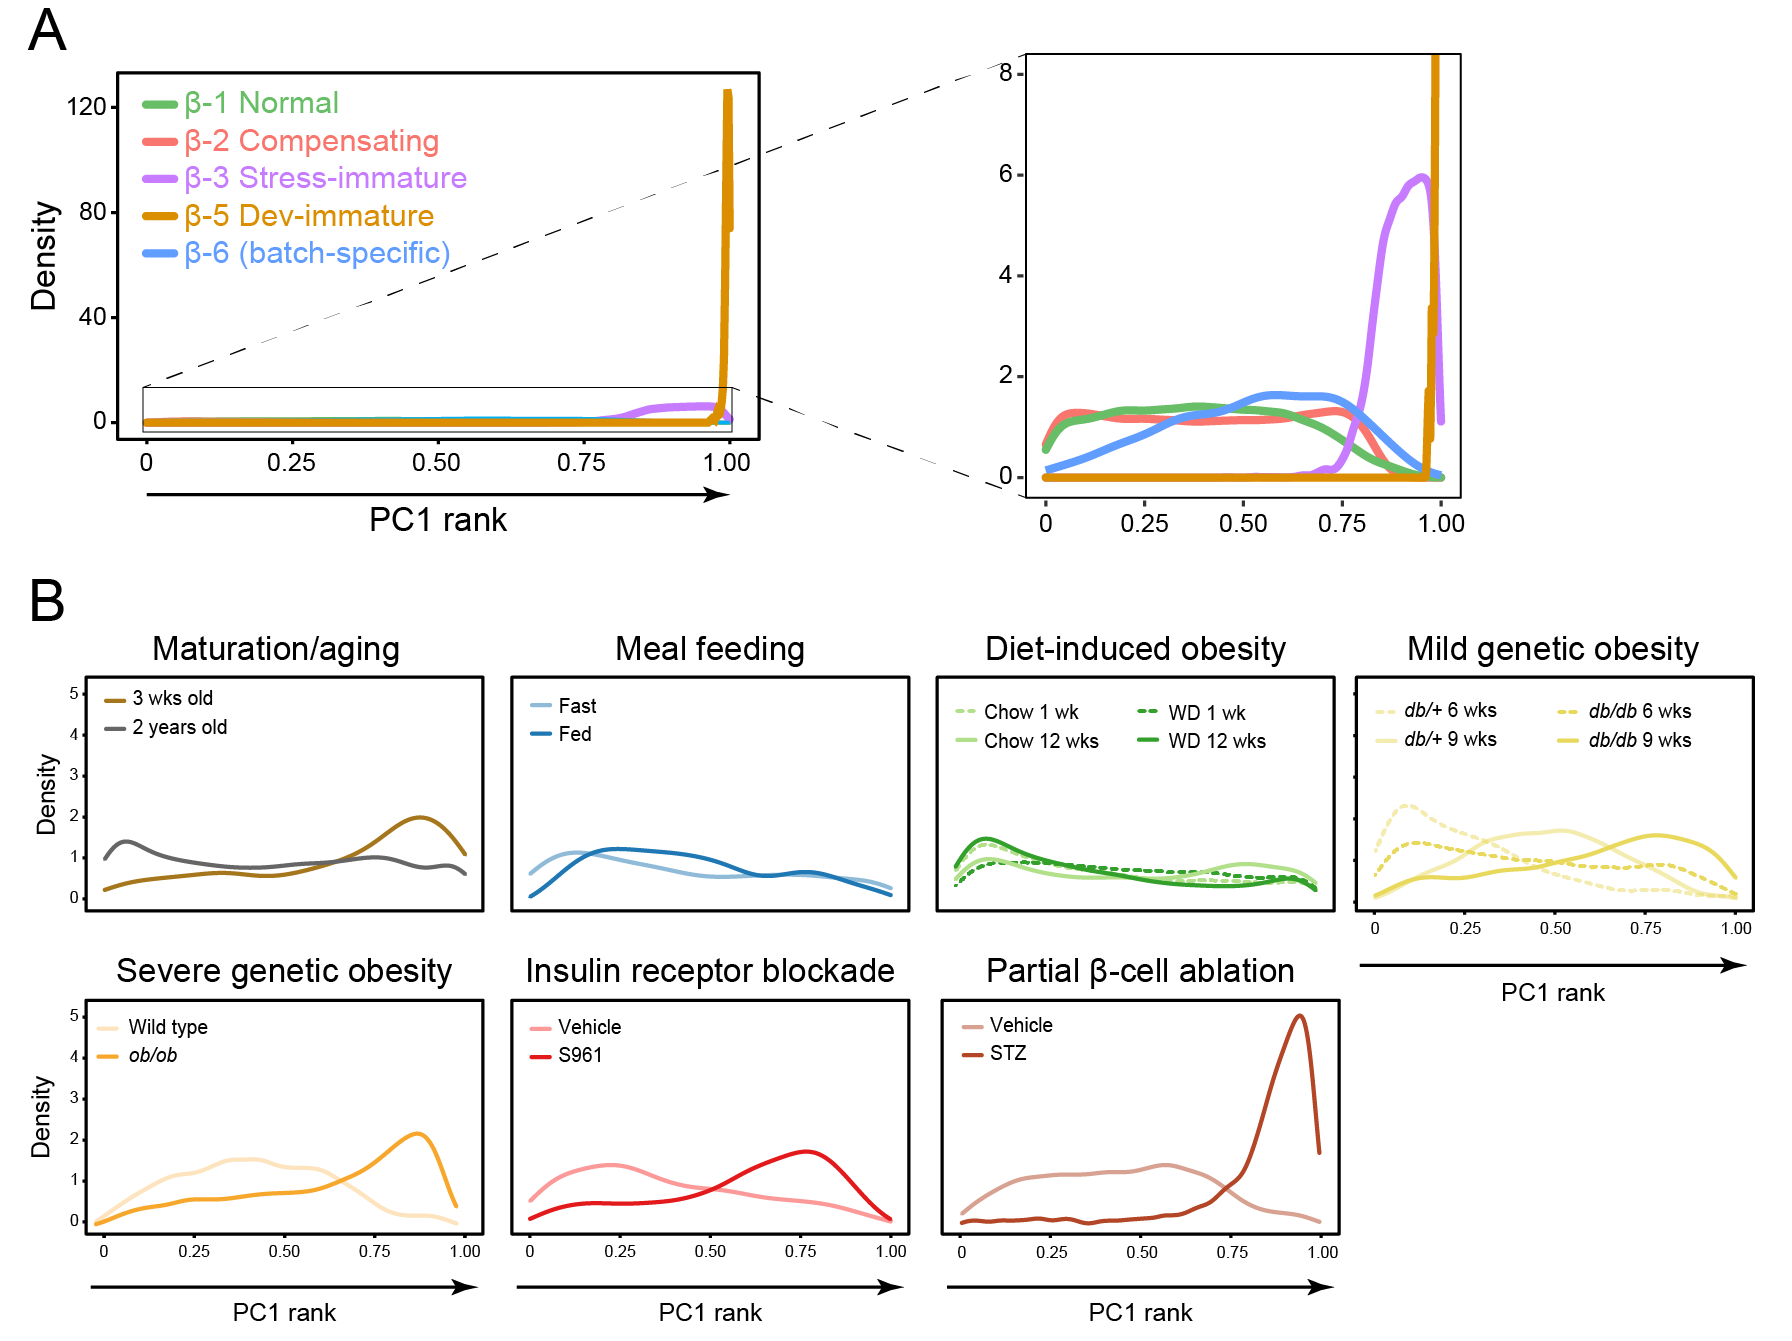
\includegraphics[width=14cm]{Appendix2/Fig/F3-7-02.png}
\caption[Loss of $\beta$-cell maturity across studies along \glsentryshort{pc}1]{\textbf{Loss of $\beta$-cell maturity across studies along \gls{pc}1.} \textbf{(A)} Density plot depicting the distribution of non-proliferating $\beta$-cell subsets as curves along normalized \gls{pc}1 rank. The inset depicts the distributions of $\beta$-1, $\beta$-2, $\beta$-3 and $\beta$-6 subsets. \textbf{(B)} Density plots depicting the distribution of $\beta$-cells from $\beta$-1, $\beta$-2 and $\beta$-3 subsets across the seven studies along \gls{pc}1. Within each dataset, the $\beta$-cells are grouped according to healthy control and the corresponding experimental sample. Metadata about the individual studies can be found in \textbf{\autoref{tab:app_chp3_study}} and the number of cells per experimental sample can be found in \textbf{\autoref{tab:app_chp3_cellnumbers}}.}
\label{fig:app_chp3_pc1}
\end{figure}


\begin{figure}[H]
\centering
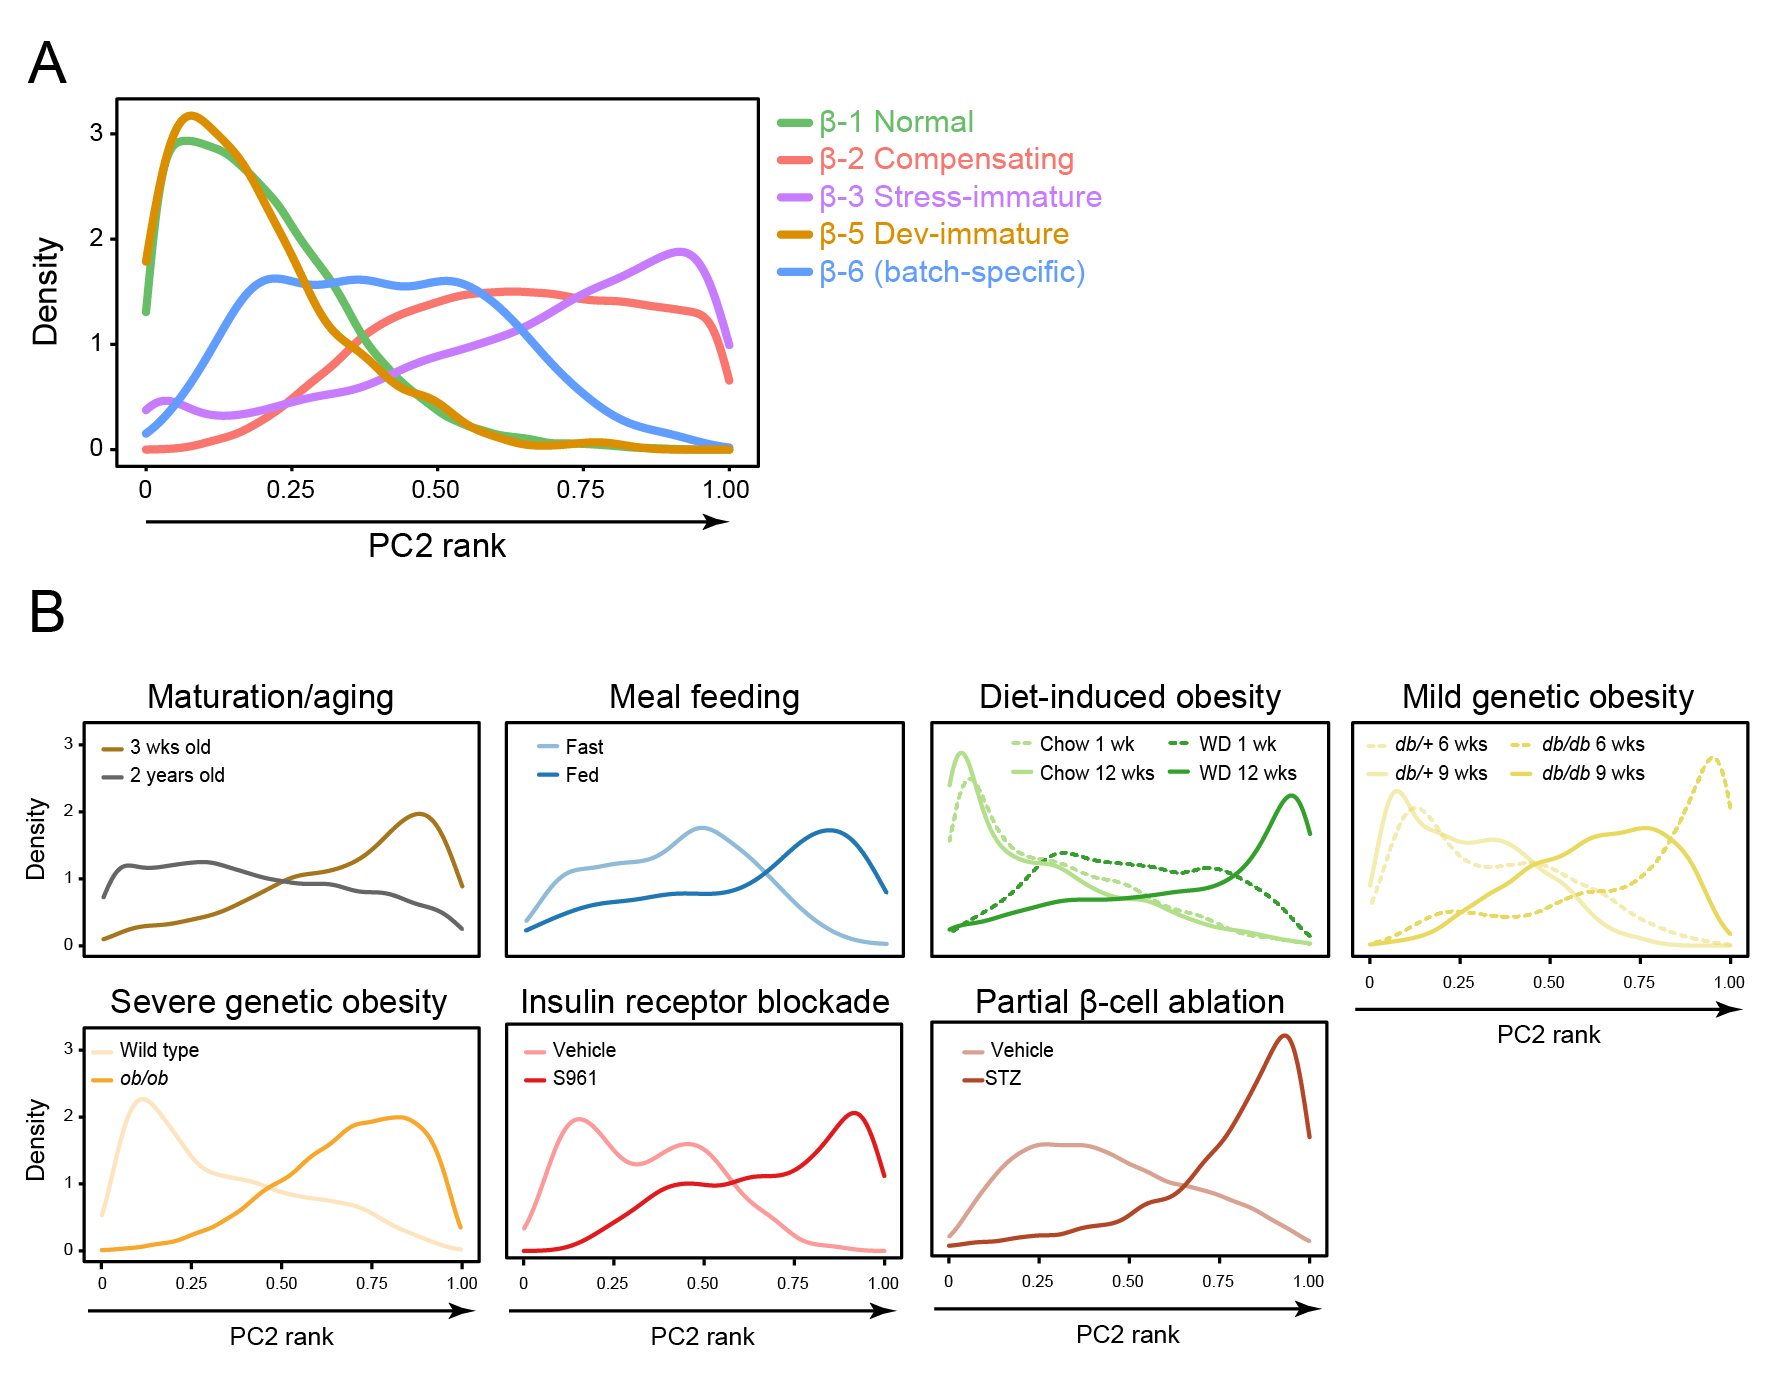
\includegraphics[width=\linewidth]{Appendix2/Fig/F3-7-03.png}
\caption[Increased $\beta$-cell workload across studies along \glsentryshort{pc}2]{\textbf{Increased $\beta$-cell workload across studies along \gls{pc}2.} \textbf{(A)} Density plot depicting the distribution of non-proliferating $\beta$-cell subsets as curves along normalized \gls{pc}2 rank. \textbf{(B)} Density plots depicting the distribution of $\beta$-cells from $\beta$-1, $\beta$-2 and $\beta$-3 subsets across the seven studies along \gls{pc}2. Within each study, the $\beta$-cells are grouped according to healthy control and the corresponding experimental sample. Metadata about the individual studies can be found in \textbf{\autoref{tab:app_chp3_study}} and the number of cells per experimental sample can be found in \textbf{\autoref{tab:app_chp3_cellnumbers}}.}
\label{fig:app_chp3_pc2}
\end{figure}


\begin{figure}[H]
\centering
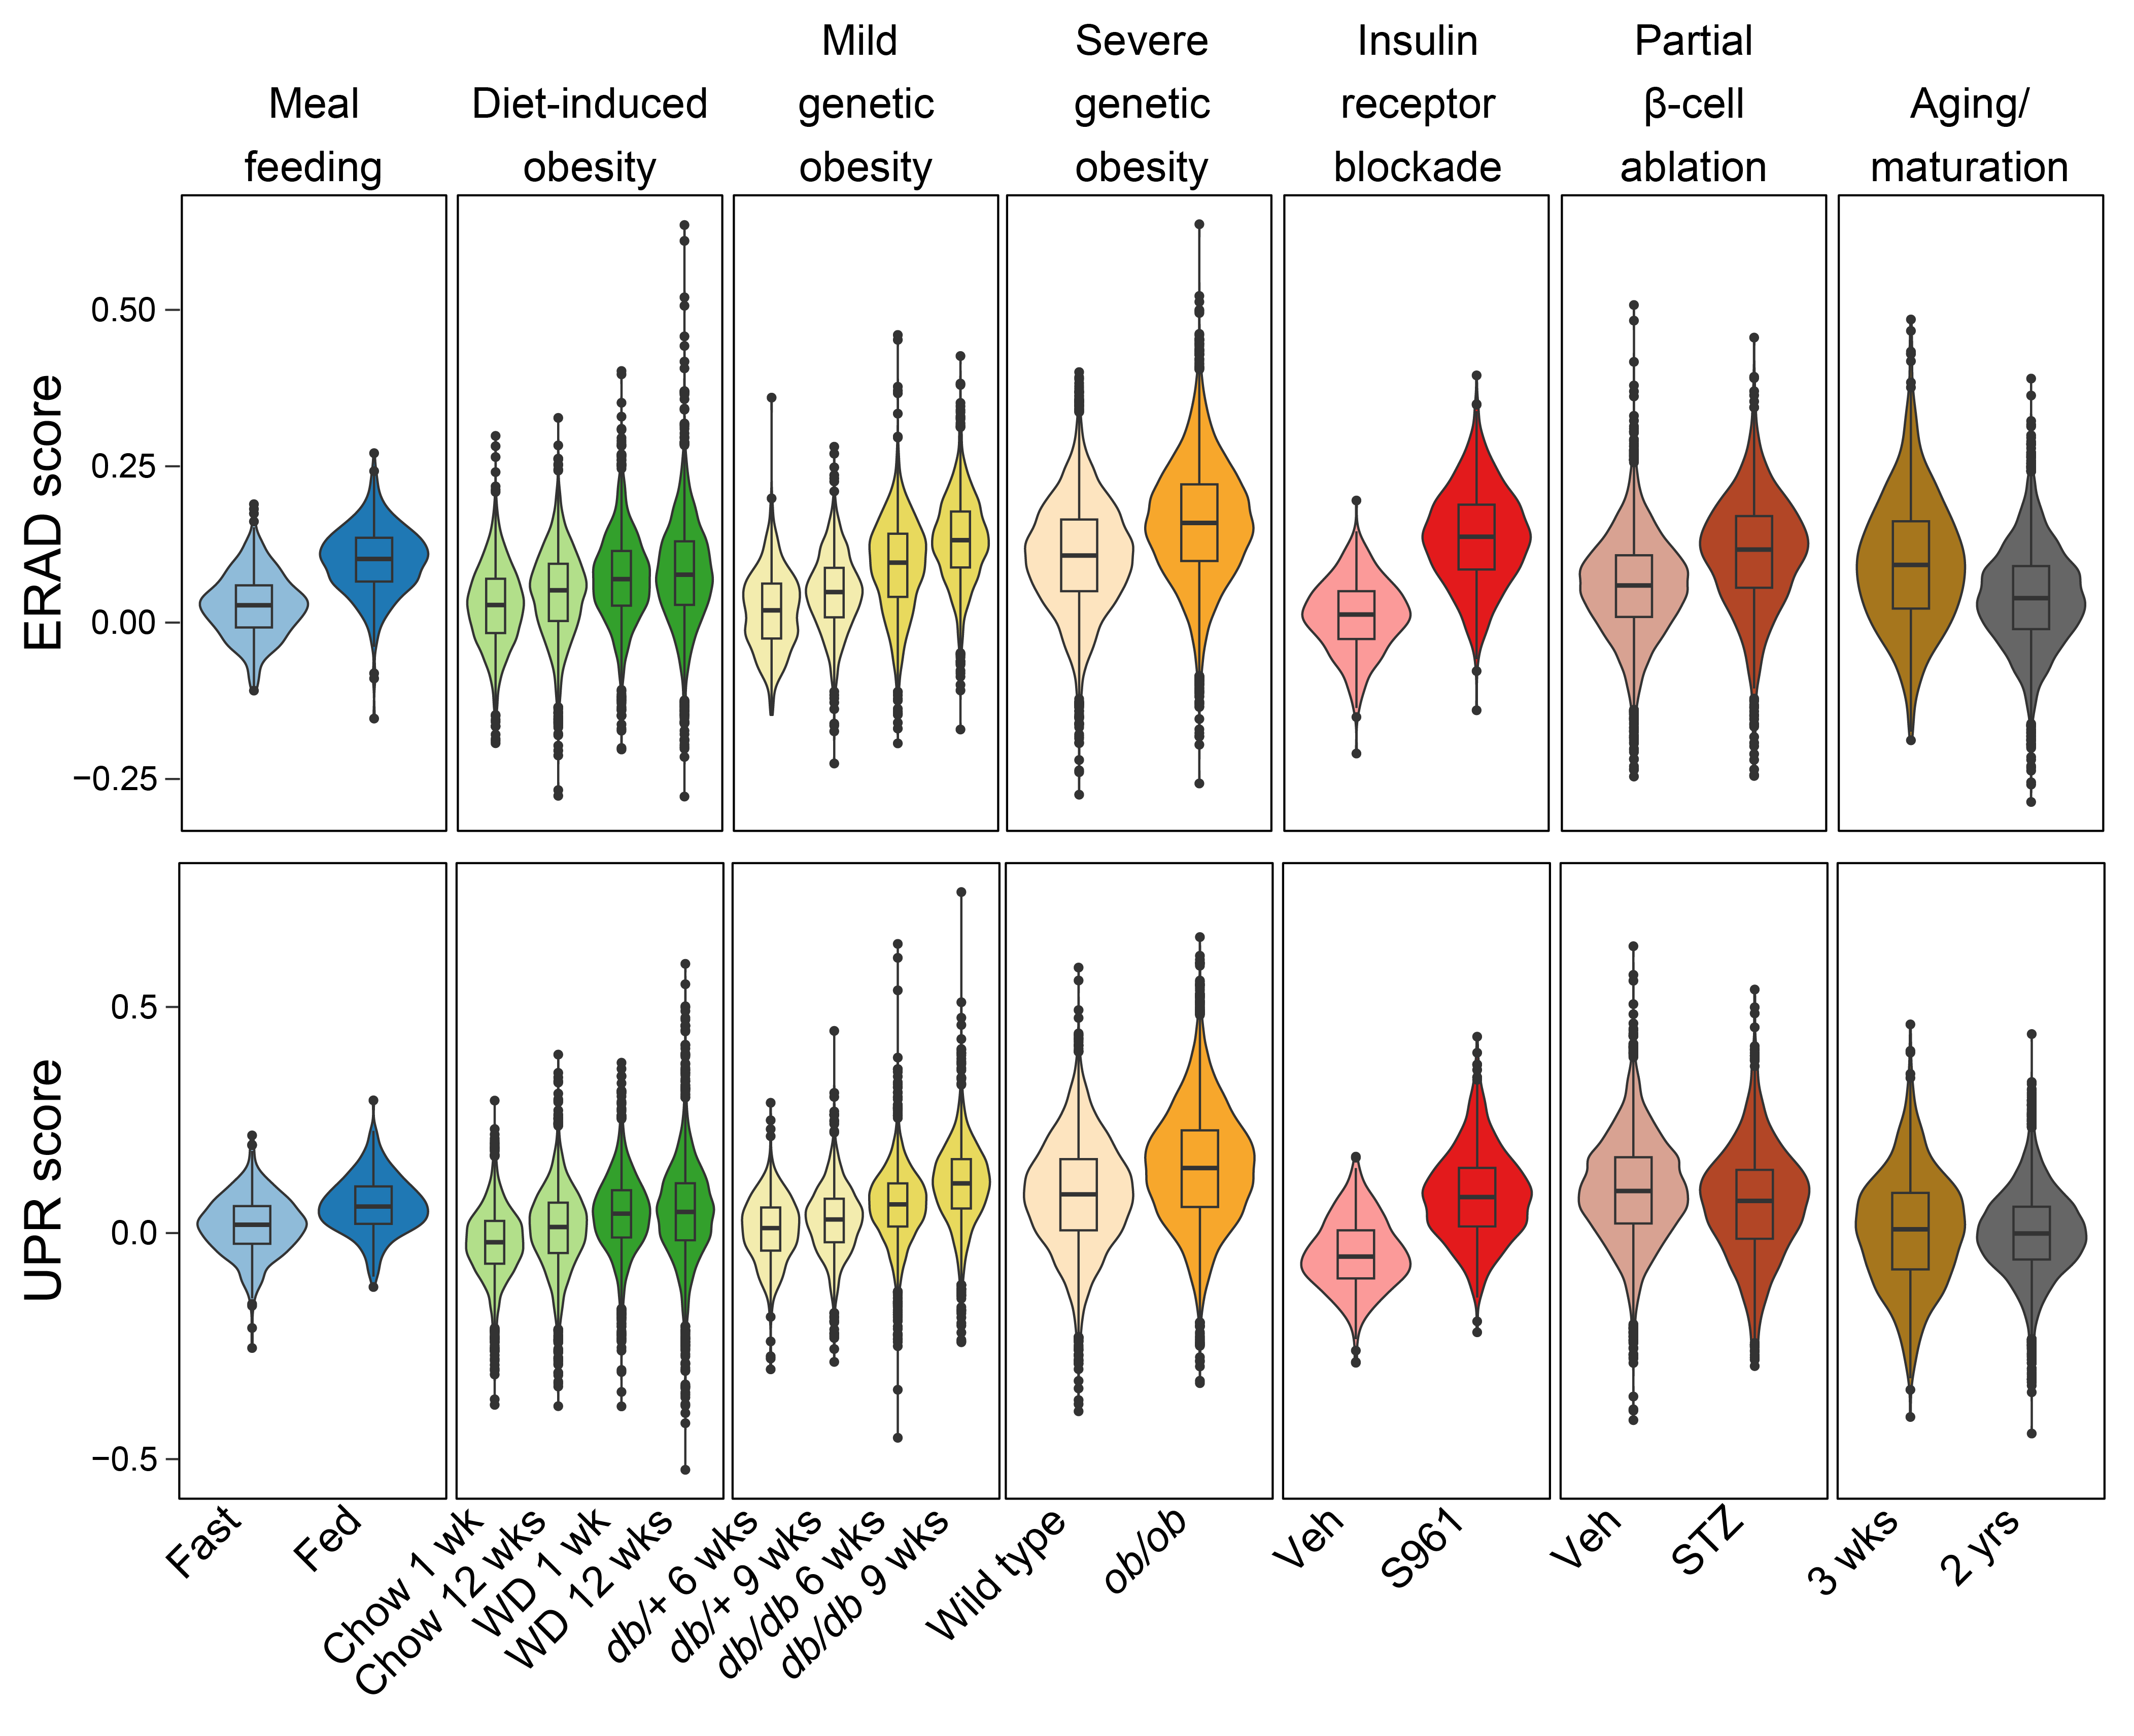
\includegraphics[width=12cm,keepaspectratio]{Appendix2/Fig/F3-22-02.png}
\caption[Module scoring of \glsentryshort{erad} and \glsentryshort{upr} gene sets across experimental samples]{\textbf{Module scoring of \gls{erad} and \gls{upr} gene sets across experimental samples.} Violin plots depicting the gene set scores for \gls{erad} (top) and \gls{upr} (bottom) processes across $\beta$-cell workload models and corresponding healthy controls from individual studies. On the overlay box plots, the middle horizontal line represents the median, the box represents the inter-quartile range and the whiskers represent the minimum and maximum values. The number of cells are indicated in \textbf{\autoref{tab:app_chp3_cellnumbers}}.}
\vspace{-25pt}
\label{fig:app_chp3_eradupr}
\end{figure}


\begin{figure}[H]
\centering
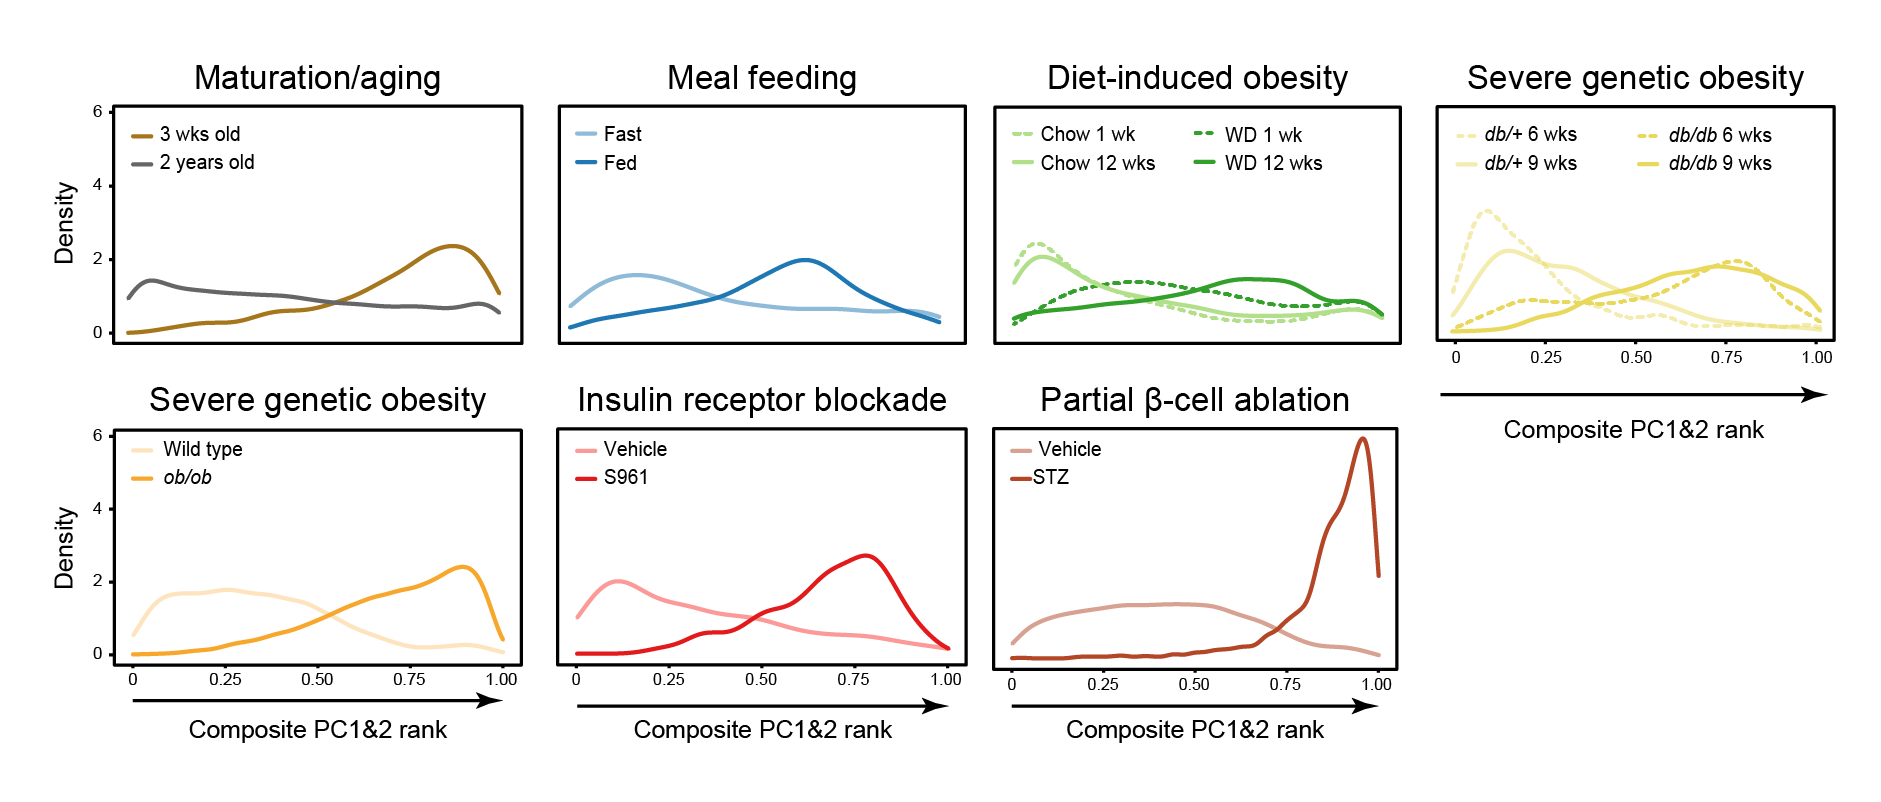
\includegraphics[width=\linewidth]{Appendix2/Fig/F3-7-01.png}
\caption[$\beta$-cell dysfunction across studies along Maturity-Workload axes]{\textbf{$\beta$-cell dysfunction across studies along composite Maturity-Workload axes.} Density plots depicting the distribution of $\beta$-cells from $\beta$-1, $\beta$-2 and $\beta$-3 subsets across the seven studies along the Maturity (\gls{pc}1) - Workload (\gls{pc}2) axes. Within each study, the $\beta$-cells are grouped according to healthy control and the corresponding experimental sample. Metadata about the individual studies can be found in \textbf{\autoref{tab:app_chp3_study}} and the number of cells per experimental sample can be found in \textbf{\autoref{tab:app_chp3_cellnumbers}}.}
\label{fig:app_chp3_pc12}
\end{figure}


\begin{figure}[H]
\centering
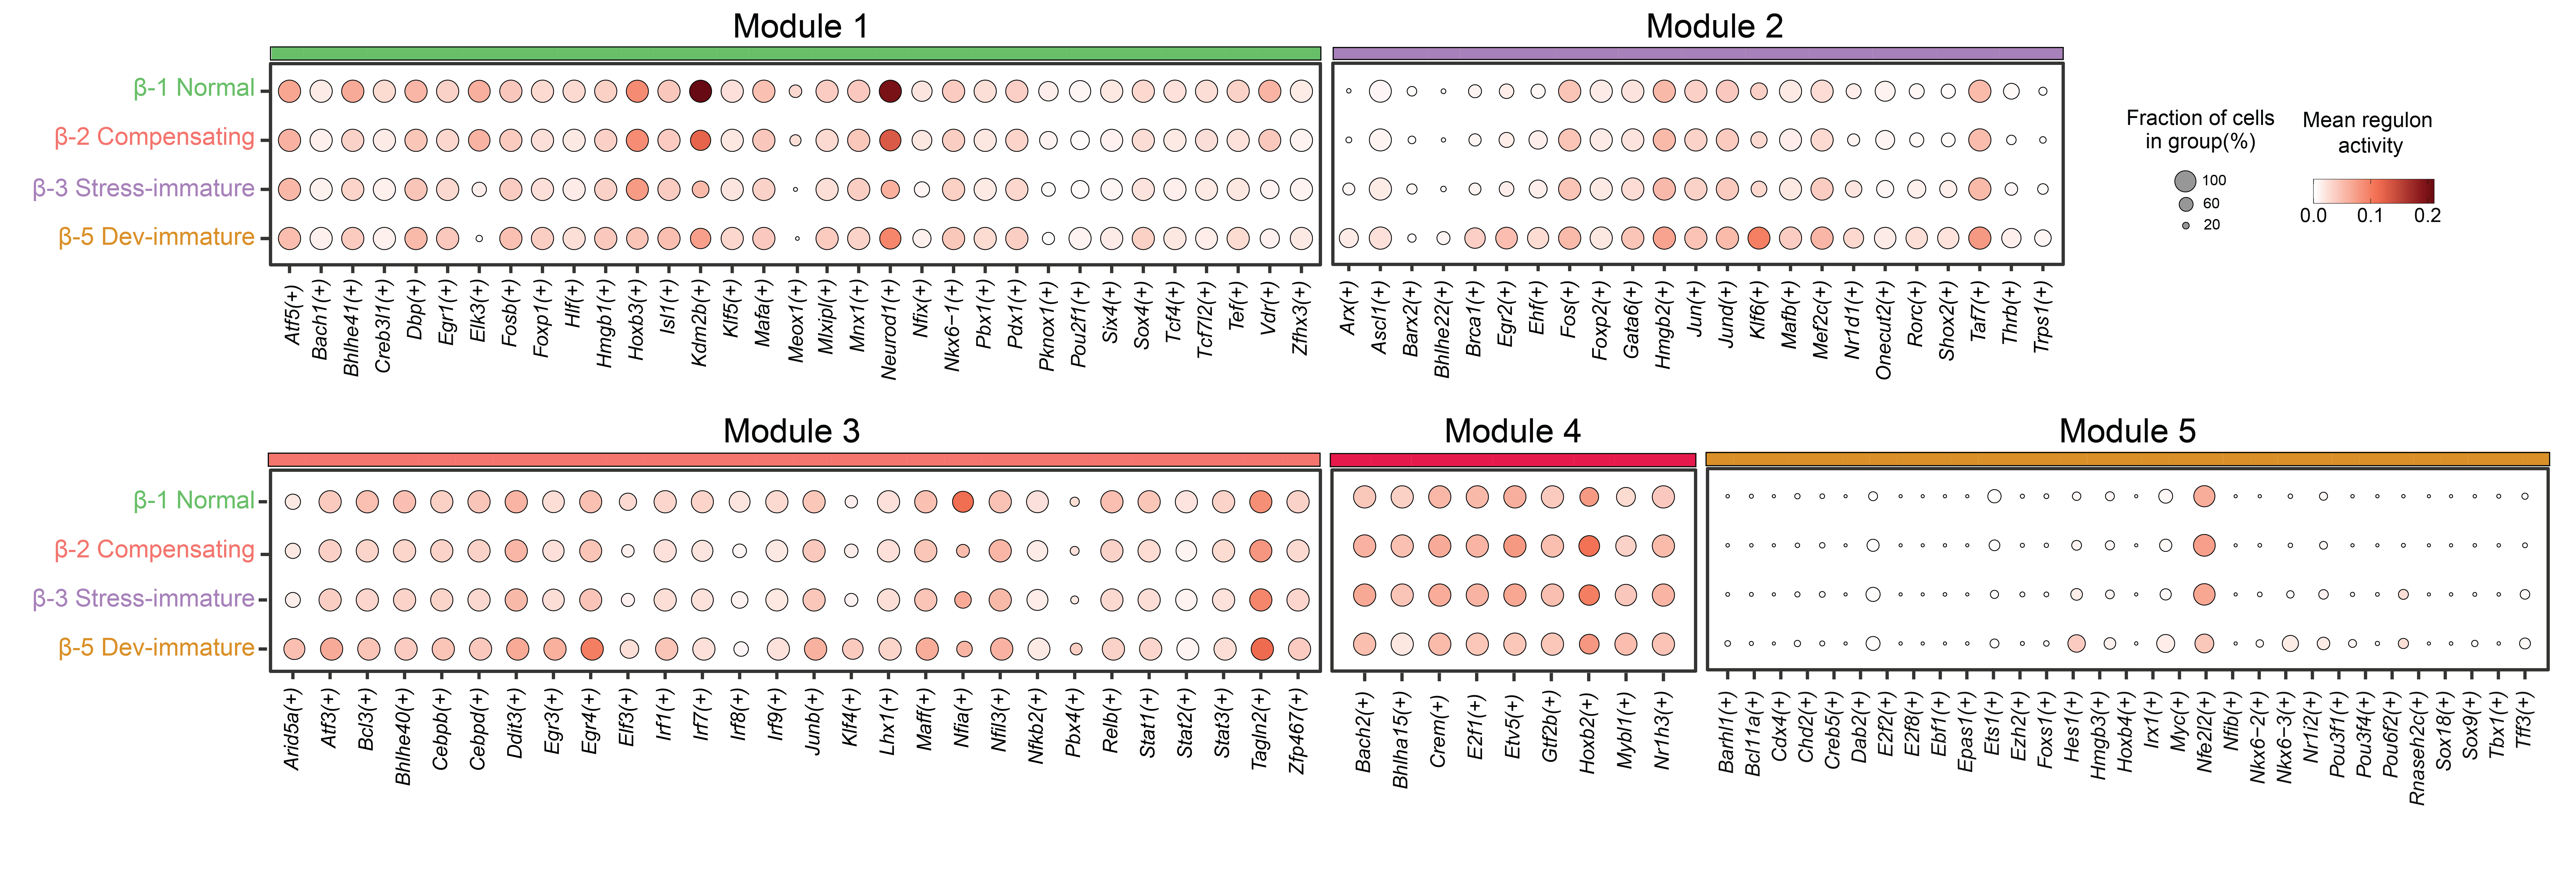
\includegraphics[width=\linewidth]{Appendix2/Fig/F3-18-01.png}
\caption[Mean activity of all identified regulons across $\beta$-cell subsets]{\textbf{Mean activity of all identified regulons across $\beta$-cell subsets.} Dot plot depicting the mean activity of all 124 regulons across $\beta$-1, $\beta$-2, $\beta$-3 and $\beta$-5 subsets. The regulons are grouped by modules identified based on hierarchical clustering of the regulons, using \glsentrylong{csi} (\glsentryshort{csi}) as a distance measure. The color of the dots indicate the mean activity and the size of the dots correspond to the fraction of cells in which the regulon is active.}
\label{fig:app_chp3_scenic_betasubsets}
\end{figure}
\vspace{-23pt}


% \mysidecaption{0.4}{%
% \captionof{figure}[Gene-set scores in Aging/maturation study]{\textbf{Scores of five gene-sets in Aging/maturation study}}%
% }
% {%
% 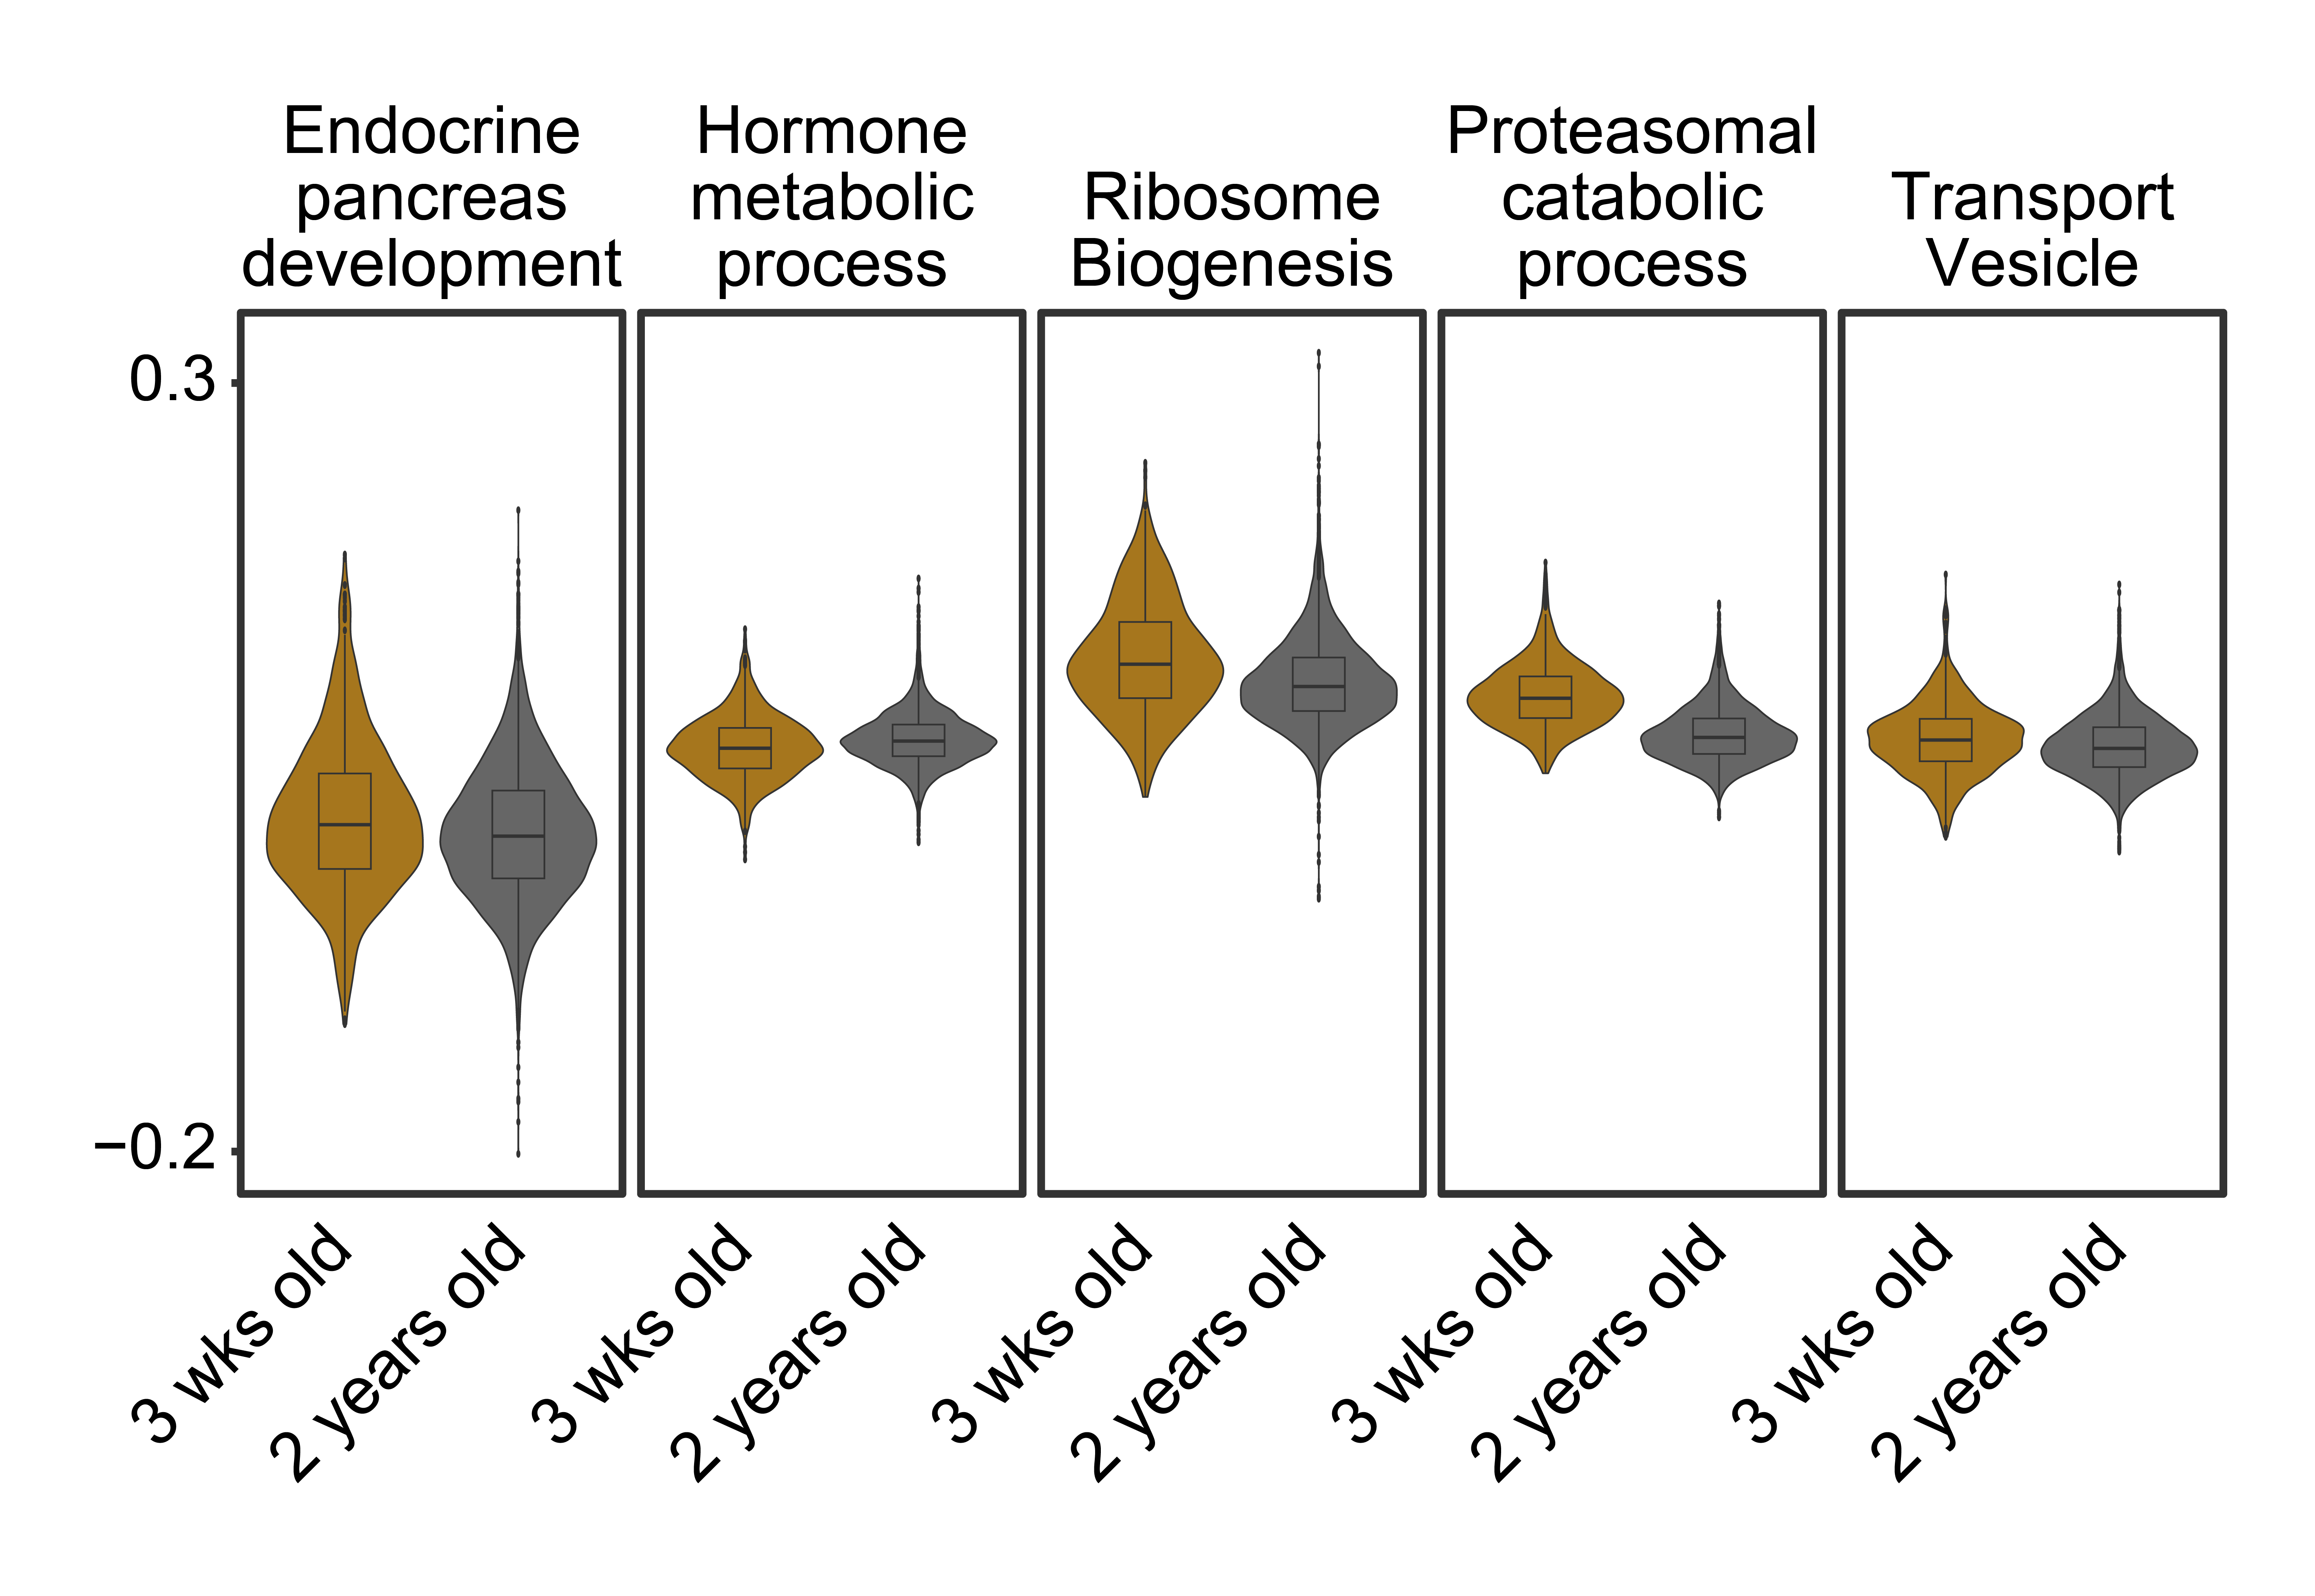
\includegraphics[width=9.5cm]{Appendix2/Fig/F3-14-01.png}%
% }[t]%

% \begin{figure}[t]
% \centering
% 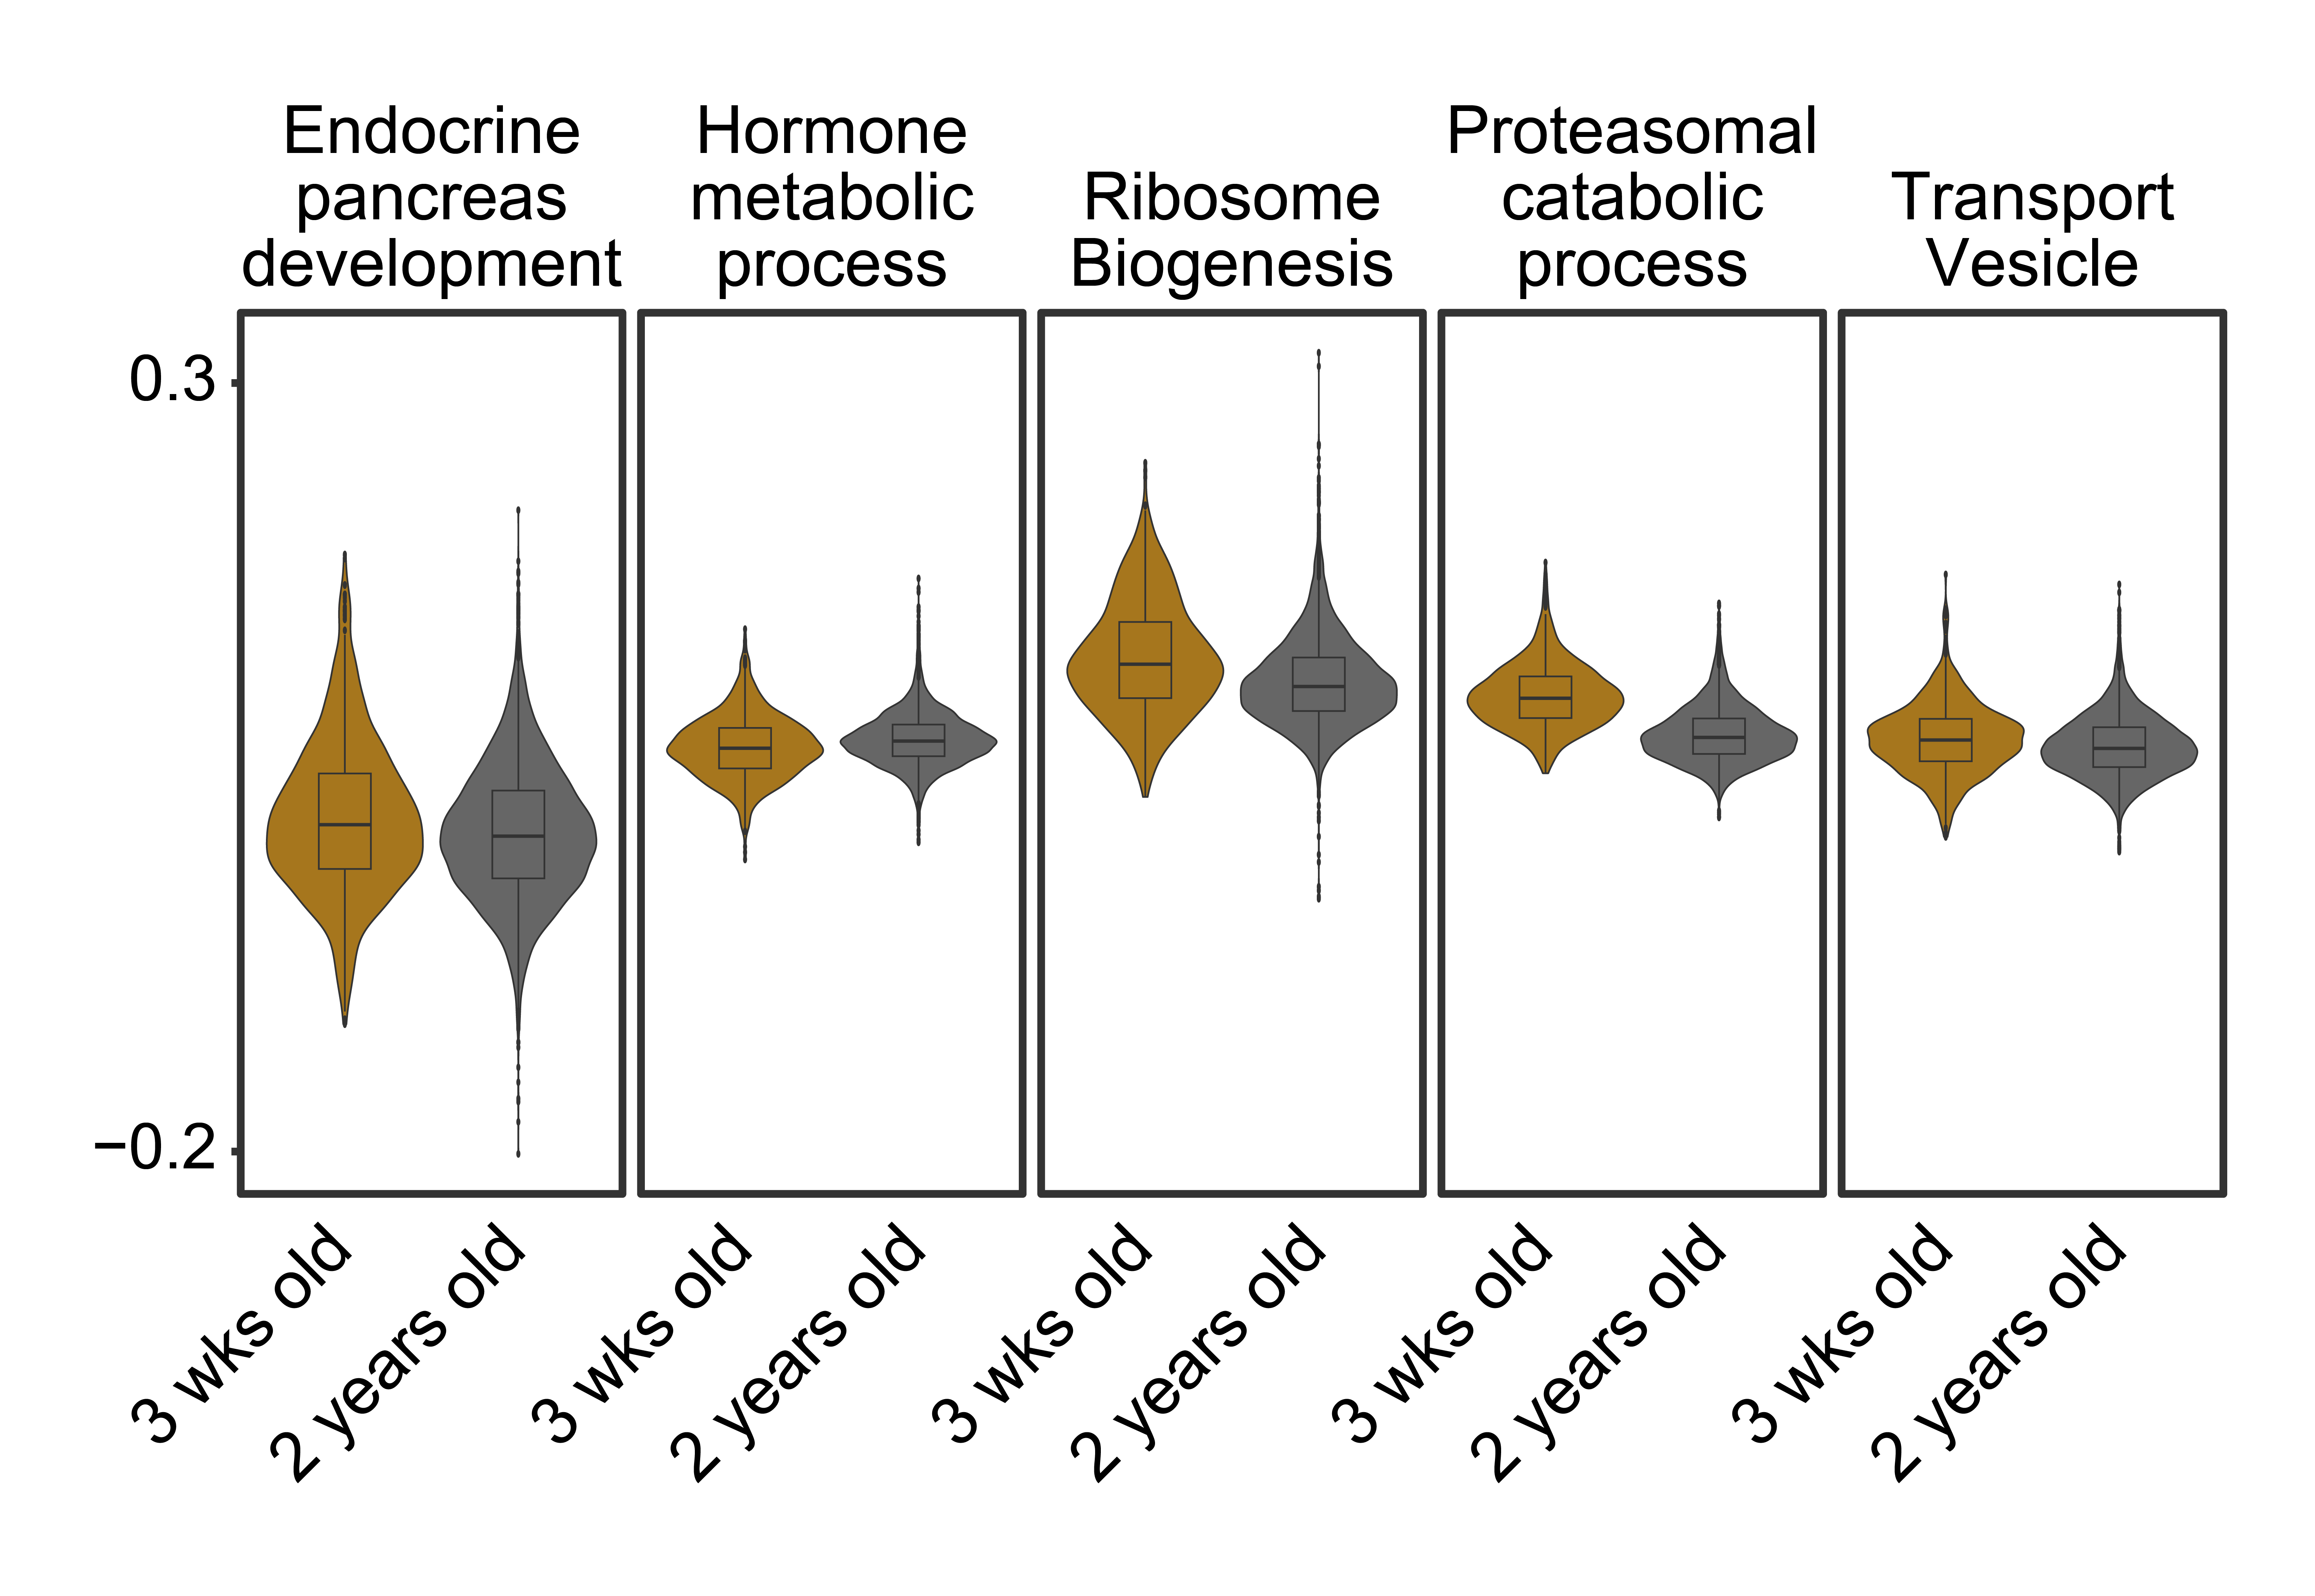
\includegraphics[width=11cm]{Appendix2/Fig/F3-14-01.png}
% \caption[]{Gene-set scores in Aging/maturation study}
% \label{suppl_fig:chp3_agingscores}
% \end{figure}




% \begin{landscape}
\begin{figure}[H]
\centering
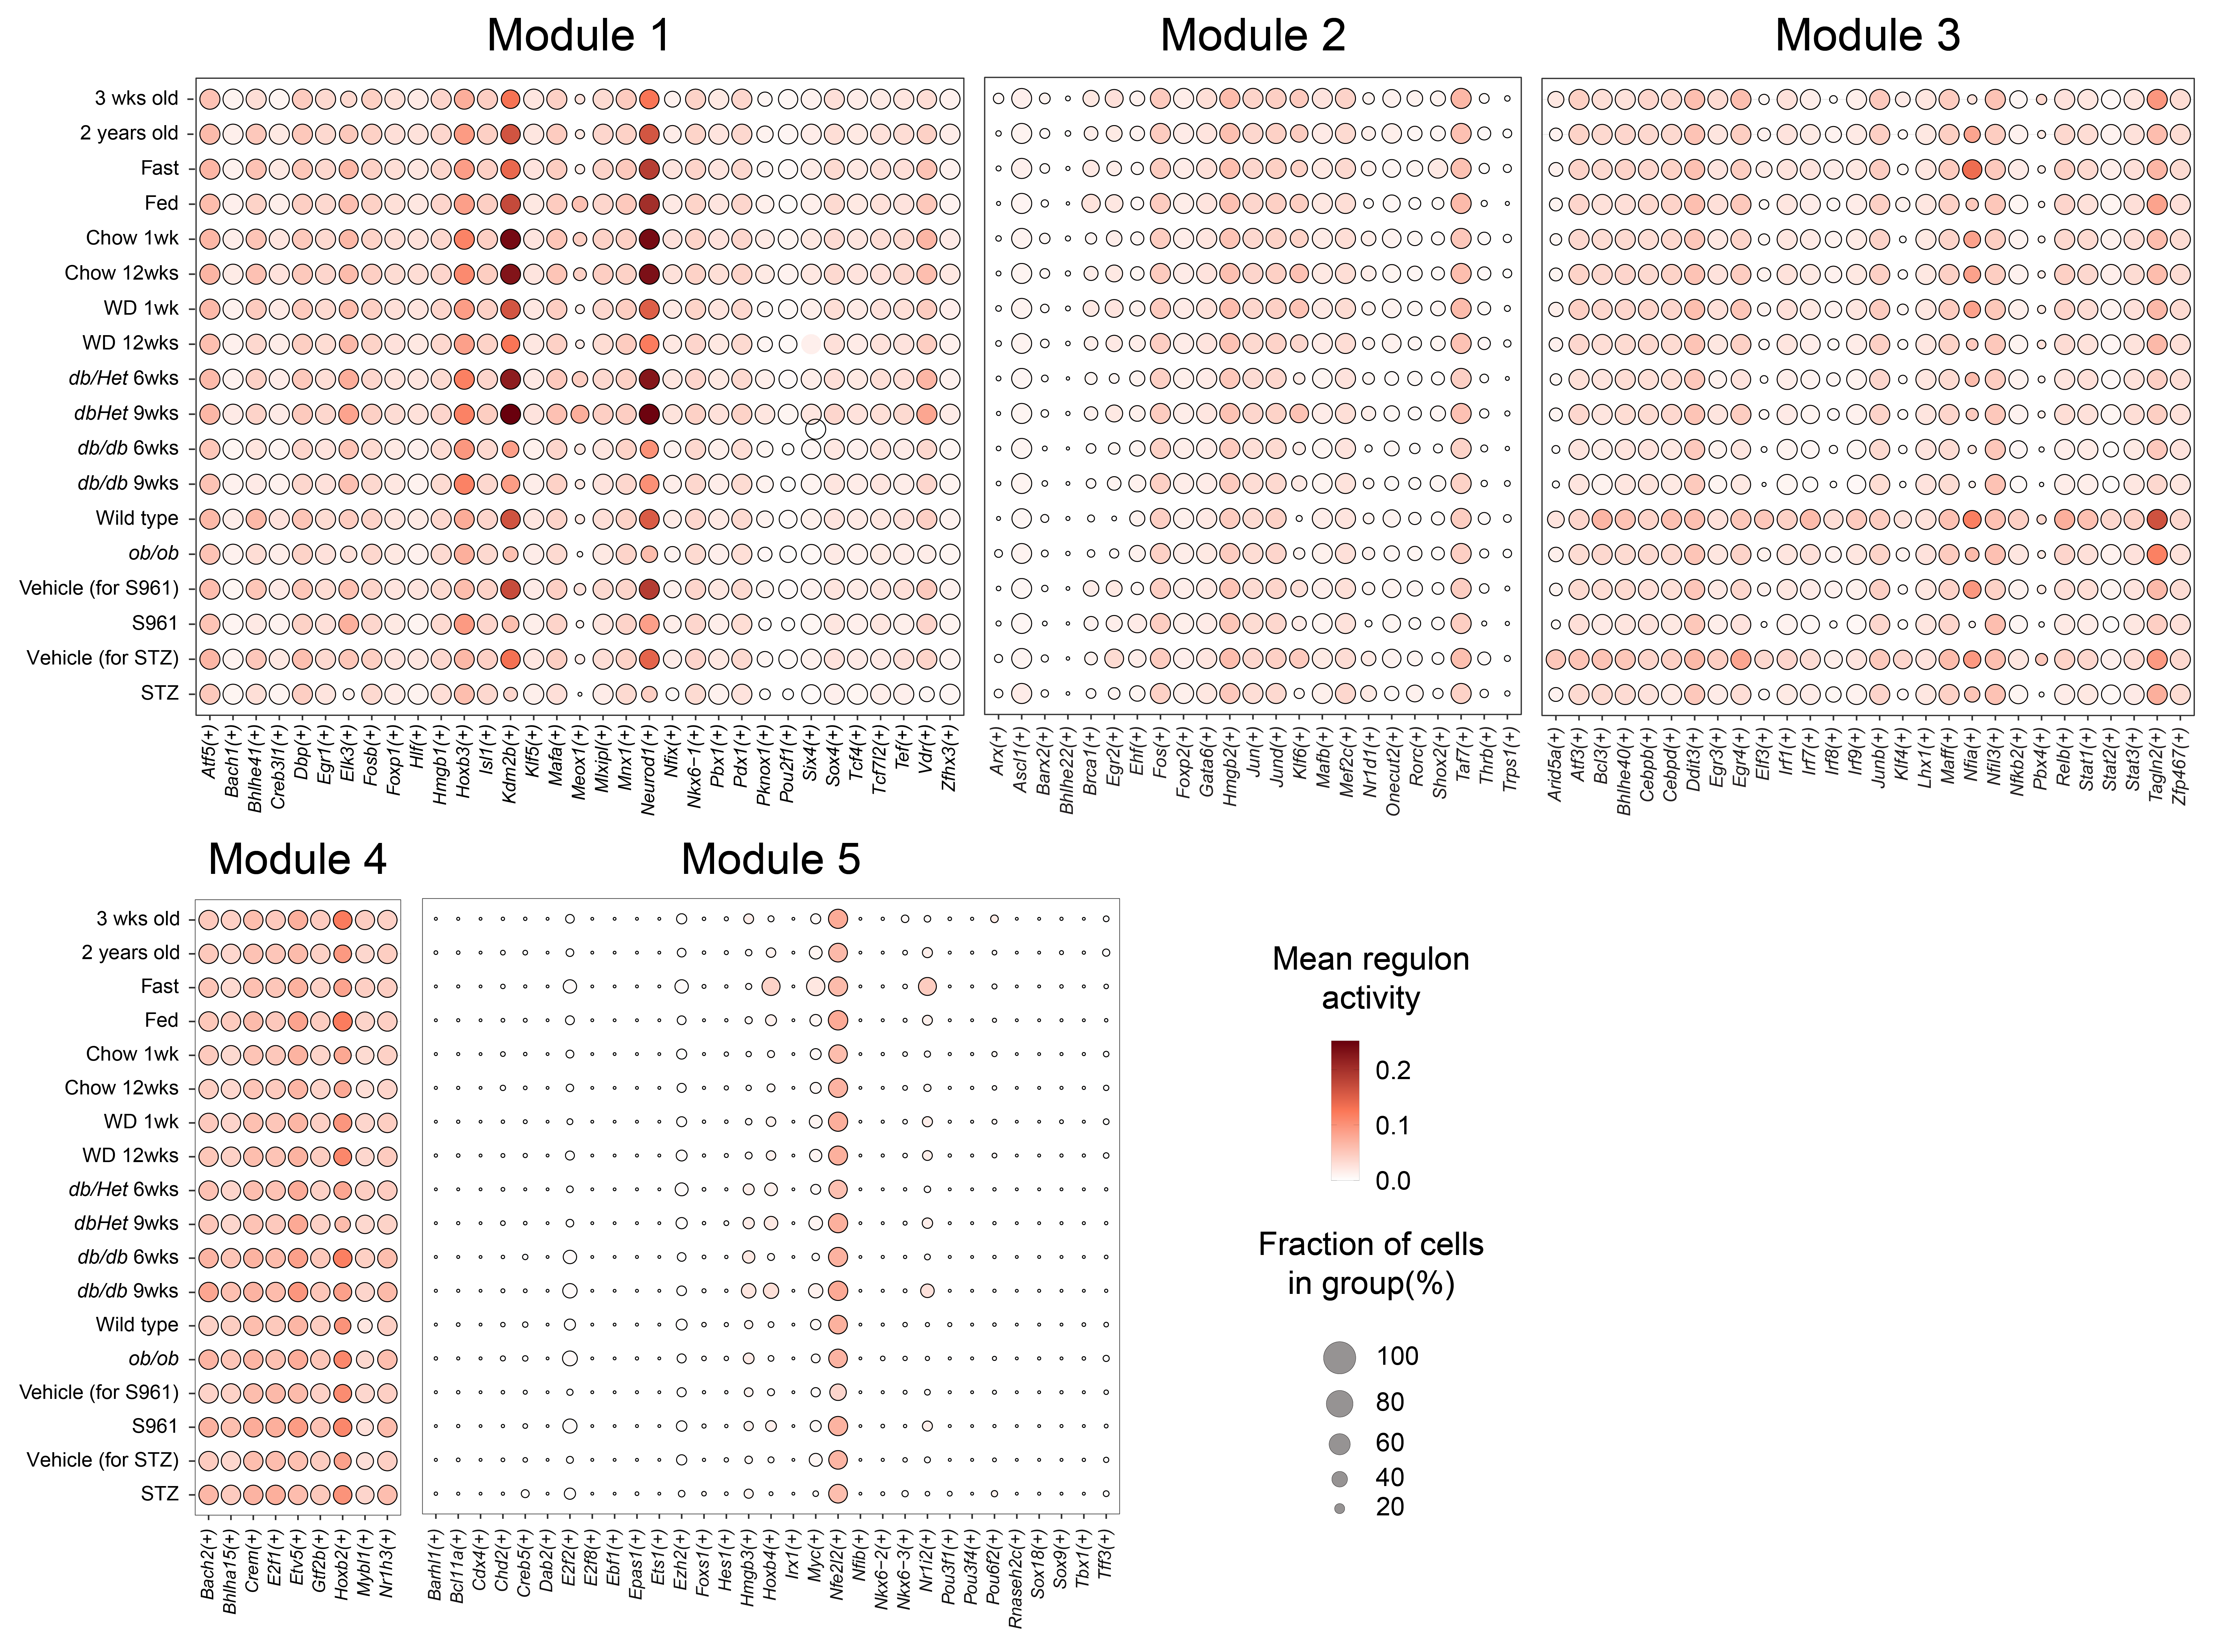
\includegraphics[width=\linewidth]{Appendix2/Fig/F3-15-01.png}
\caption[Mean activity of all identified regulons across experimental samples]{\textbf{Mean activity of all identified regulons across experimental samples.} Dot plot depicting the mean activity of all 124 regulons across all experimental samples included in the integrated atlas. The regulons are grouped by modules identified based on hierarchical clustering of the regulons, using \glsentrylong{csi} (\glsentryshort{csi}) as a distance measure. The color of the dots indicate the mean activity and the size of the dots correspond to the fraction of cells in which the regulon is active.}
\label{fig:app_chp3_scenic_studies}
\end{figure}
% \end{landscape}

%\end{comment}